  % % GitHub cvitanov/reducesymm/tingnan/blog.tex   pdflatex blog
                        %% logical setup, no need to edit %%%%%%%%%%
                        \newif\ifpaper \newif\ifPDF               %%
                        \newif\ifOUP \newif\ifboyscout            %%
                        \newif\ifdasbuch                          %%
                        \newif\ifsolutions                        %%
                        \dasbuchfalse %% not DasBuch, not QFT lectures %%
                        \boyscouttrue %% commented, WWW/boyscouts %%
                        \solutionstrue %% include solutions       %%
                        \paperfalse\PDFtrue %% hyperlinked        %%
                        \OUPfalse                %% ChaosBook %%%%%%
    % Toggle between draft and non-draft versions
%\boyscoutfalse                 % public, for hyperlinked ChaosBook/projects
    % Toggle between draft and non-draft
%\articletrue                   %editing the article (May 2012: nonesuch)
%\articletrue\boyscoutfalse     % article for submission

% Predrag 2013-02-17 search for "uncomment" to make Gable parts visible
%                    transfer chaosbook/soluMaps toCB: Gable's solutions

\documentclass[10pt,openany]{book}
\usepackage{amsmath,amsfonts,amssymb}
\usepackage[nooneline]{caption} % Grigo figures?
\usepackage{color}
\usepackage{url}
\usepackage{fancyhdr}
\usepackage{alltt}
\usepackage{ifthen}
\usepackage{bm}
\usepackage[latin1]{inputenc}
\usepackage[T1]{fontenc}
\usepackage{times}
\usepackage[pdftex]{graphicx}
\usepackage{array}
\providecommand\phantomsection{} % with this it works without hyperref as well
\usepackage{verbatim}
%% elton/inputs/layout.tex
% $Author: predrag $ $Date: 2015-01-26 12:59:28 -0500 (Mon, 26 Jan 2015) $

% from ChaosBook                        Predrag          5jun2008

%%%%%%%% for figure layouts:
%% fine tuning floatingfigure \usepackage[nooneline] captions %%%%%
%        \renewcommand{\captionfont}{\footnotesize} % \sffamily}
%        \renewcommand{\captionlabelfont}{\footnotesize \bfseries \rmfamily}
%        % \renewcommand{\captionlabeldelim}{.\quad}
%        % \setlength{\captionmargin}{10pt}

% \FIG{#1}    % \includegraphics[width=0.40\textwidth]{Fig/f_name.ps}  ...
%     {#2}    % short caption text omitted here
%     {#3}    % full caption text
%     {#4}    % f-figure-label
\newcommand{\FIG}[4]{\begin{widefigure}[t]{#4}
    \widefigparts{\begin{minipage}[b]{0.98\textwidth}
                    #1\end{minipage}}{#3}\end{widefigure}}

\newcommand{\FFIG}[5]{\begin{floatingfigure}[v]{0.40\textwidth}
                      \noindent
                      \includegraphics[#1]{#2}
                      \caption[#3]{#4}
                      \label{#5}
              \end{floatingfigure} }

%   \BFIG{#1}   % width=#1\textwidth
%        {#2}   % f_name.ps
%    {#3}   % short caption text
%    {#4}   % full caption text
%    {#5}   % f-figure-label
%       defined here:
\newcommand{\BFIG}[5]{\begin{figure}
              \hspace*{0.10\textwidth}%
              \begin{minipage}[b]{1.00\textwidth}
              \centering{
                      \includegraphics[width=#1\textwidth]{Fig/#2}
                     }
                      \caption[#3]{#4}
                      \label{#5}
              \end{minipage}
              \end{figure} }

%  \SFIG{#1}    % f_name.png (or .pdf)
%       {#2}    % short caption text
%       {#3}    % full caption text
%       {#4}    % f-figure-label
\newcommand{\SFIG}[4]{\begin{figure}[ht]
              %\hspace*{-0.10\textwidth}
              \hspace*{0.10\textwidth}
              \begin{minipage}[b]{0.55\textwidth}
                      \caption[#2]{#3}
                      \label{#4}
              \end{minipage}~~~~~%
              \begin{minipage}[b]{0.40\textwidth}
                      \includegraphics[width=1.00\textwidth]{#1}
              \end{minipage}
              %\hfill
              \end{figure} }

% % added by MF 2015-01-26 % % % %
\theoremstyle{definition}
\newtheorem{theorem}{Theorem}
% % % % % % % % % %


%%%%%%%%%%%%%%% FORMATING: PAGINATION FOR bin/mkbook %%%%%%%%%%%%%%%%%%%%%%%

\newcommand{\Resume}{\section*{\textsf{\textbf{R\'esum\'e}}}
    %   \addcontentsline{toc}{section}{{~~~~Resum\'e}}
                \addtocontents{toc}{{\small r\'esum\'e \thepage ~}} }
\newcommand{\ResumeEnd}{}

\newcommand{\Remarks}{\section*{\textsf{\textbf{Commentary}}}
        \addtocontents{toc}{{\small commentary \thepage ~ }} }
\newcommand{\RemarksEnd}{\ifOUP   %\end{enumerate}
        \end{reading} \else  \fi}

\newcommand{\Problems}[2]{
                \renewcommand{\inputfile}{#1 -  #2}
    \ifboyscout \begin{exercisesBS} \else \begin{exercises} \fi
    \begin{enumerate}}
\newcommand{\ProblemsEnd}{\end{enumerate}
    \ifboyscout \end{exercisesBS} \else \end{exercises} \fi}

\newcommand{\Solution}[4]{
        \section*{Chapter~\ref{c-#1}. #4}
                \renewcommand{\inputfile}{#2 -  #3}
        % PC:  modified 28 may 2000
                %         \renewcommand{\chapName}{#1}
                %        \setcounter{startSect}{\thepage}
                        }
\newcommand{\Solutions}{
        \section{\textsf{\textbf{Solutions}}}
        %\addcontentsline{toc}{section}{{~~~~Solutions}}
                        }


%%%%%%%%%%%%%%% NUMBERED ENVIRONMENTS %%%%%%%%%%%%%%%%%%%%%%%%%%%%%%%
% REPLACE {13.5cm} by \textwidth counter in these environments
\newtheorem{exerc}{\textsf{\textbf{Exercise}}}[chapter]
% \newtheorem{exerc}{}[chapter]
% \newtheorem{exerc}{{$\bullet$}}[chapter]
 \newcommand{\exercise}[2]{
        %\vskip -13mm
         \noindent
         \begin{exerc}{
\renewcommand{\theenumi}{\alph{enumi}}
\renewcommand{\labelenumi}{\textbf{(\alph{enumi})\ }}
    {\noindent\small
         ~~\textsf{\textbf{#1}} ~
           \slshape\sffamily{#2}  } % \textsl would not work...
    }
         \vskip -1mm
% removed the line: % \noindent\rule[.1mm]{\linewidth}{.5mm}
         \end{exerc}
                          }

\newcommand{\Exercise}[2]{      %environment for obligatory problems
        %\vskip -13mm
        \noindent
        \begin{exerc}{
\renewcommand{\theenumi}{\alph{enumi}}
\renewcommand{\labelenumi}
    {\textsf{\textbf{ (\alph{enumi})\ }}}
        {\noindent
         ~~\textsf{\textbf{\underline{#1}}} ~
           \slshape\sffamily{#2}  } % \textsl would not work...
        }
         \vskip -1mm
        \end{exerc}
                          }

\newcommand{\solution}[3]{
        {\noindent\small
         \textsf{\textbf{Solution \ref{#1}~-~#2}} %LABEL - TITLE
         \slshape\sffamily{#3}                    %TEXT
         }
         \vskip  1ex  %4mm
% removed the line: % \noindent\rule[.1mm]{\linewidth}{.5mm}
                        }
\newcommand{\exerbox}[1]
{\marginpar[{\color{red}\sf\footnotesize\hfill exercise \ref{#1} }]
               {\color{red}\sf\footnotesize exercise \ref{#1} \hfill}}

\newtheorem{exmple}{\noindent\small\textsf{\textbf{Example}}}[chapter]
\newcommand{\example}[2]{
    \vskip -13mm
        %\begin{offset}
        \begin{exmple}
           \noindent\small
           \textsf{\textbf{#1}} ~
       \slshape\sffamily{#2}
       % \textsl would not work...
    \end{exmple}
    %\end{offset}
        \vskip -1mm
             }

\newtheorem{rmark}{{\small\textsf{\textbf{Remark}}}}[chapter]
\newcommand{\remark}[2]{
        % \begin{quotation}
        \begin{rmark}
        {\small\em\noindent {\small\sf \underline{ #1} ~} #2 }
    \end{rmark}
    % \end{quotation}
              }
         %% page layout, ChaosBook environments
%%%%%%%%%%%%%%%%%%%%%%%%%%%%%%%%%%%%%%%%%%%%%%%%%%%%%%%%%%%%%%
% GitHub cvitanov/reducesymm/inputs/setupSveZha.tex
% $Author$ $Date$
% Predrag                                       2014-04-18

\usepackage[latin1]{inputenc}
\usepackage[T1]{fontenc}
\usepackage{times}
\usepackage[pdftex]{graphicx}
\usepackage{array}
\usepackage{verbatim}
\usepackage[pdftex,colorlinks]{hyperref}
\usepackage{amsmath}

\hypersetup{
   pdfauthor=Tingnan Zhang
   pdfkeywords=deterministic diffusion,
   pdftitle=Cycle averaging formulas applied to a periodic Lorentz gas
            }

\graphicspath{{../figs/}{../tingnan/figs/}{../Fig/}{ChaosBook/}}  %% directories with graphics

  % % GitHub cvitanov/reducesymm/inputs/biblatex.tex

% Predrag 2015-11-27 activate hyperlinks for journals and URL's

%%%%%%%%%%%%%%%%%%%%%% need elsewhere in the master file %%%%%%%%%%%%%%%%%%%%%%%%%%
   %%%%%%%%%%%%%%%%%%%%%% in the header:
% \usepackage[pdftex,colorlinks]{hyperref}
%   % % GitHub cvitanov/reducesymm/inputs/biblatex.tex

% Predrag 2015-11-27 activate hyperlinks for journals and URL's

%%%%%%%%%%%%%%%%%%%%%% need elsewhere in the master file %%%%%%%%%%%%%%%%%%%%%%%%%%
   %%%%%%%%%%%%%%%%%%%%%% in the header:
% \usepackage[pdftex,colorlinks]{hyperref}
%   % % GitHub cvitanov/reducesymm/inputs/biblatex.tex

% Predrag 2015-11-27 activate hyperlinks for journals and URL's

%%%%%%%%%%%%%%%%%%%%%% need elsewhere in the master file %%%%%%%%%%%%%%%%%%%%%%%%%%
   %%%%%%%%%%%%%%%%%%%%%% in the header:
% \usepackage[pdftex,colorlinks]{hyperref}
% \input{../inputs/biblatex}
% \addbibresource{../bibtex/xxx1.bib}
% \addbibresource{../bibtex/xxx2.bib}
   %%%%%%%%%%%%%%%%%%%%%% in the body, presumably at the very end:
% replace
%   \bibliographystyle{../inputs/adkPCphysrev} % (or whichever .bst style)
%   \bibliography{../bibtex/siminos}
% by
% \printbibliography[
% heading=bibintoc,
% title={References}
% 				  ] %, type=online]  % if not using default "Bibliography"
%%%%%%%%%%%%%%%%%%%%%%%%%%%%%%%%%%%%%%%%%%%%%%%%%%%%%%%%%%%%%


%%%%%%%%%%%%%%%%%%  BIBLATEX MACROS %%%%%%%%%%%%%%%%%%%%%%%%%%%%%%%%
    % AIP, APS style source: https://github.com/josephwright/biblatex-phys
\usepackage[
    backend=bibtex,
    sorting=nyt,
    style=numeric, %alphabetic, % %style=authoryear,
    natbib=true, %false, %
    style=phys, % aps
    biblabel= superscript, % brackets, %
    articletitle=true,  % false, % aps
    chaptertitle=true,  % aip;  % false, % aps
    pageranges = true , % aip: the full range
             % = false, % aps: only the first page being printed
    sortlocale=en_US,
    firstinits=true,
    url=false, %true,  %
    doi=false, %true,
    eprint=false
            ]{biblatex}
%\AtEveryBibitem{\clearfield{issn}} \AtEveryCitekey{\clearfield{issn}}
%\ExecuteBibliographyOptions{doi=false}
%\newbibmacro{string+doi}[1]{%
%  \iffieldundef{doi}{#1}{\href{http://dx.doi.org/\thefield{doi}}{#1}}}
%\DeclareFieldFormat{title}{\usebibmacro{string+doi}{\mkbibemph{#1}}}
%\DeclareFieldFormat[article]{title}{\usebibmacro{string+doi}{\mkbibquote{#1}}}

    % http://tex.stackexchange.com/questions/133373/biblatex-adding-url-to-techreport-title-doesnt-work/133374#133374
\DeclareFieldFormat
  [article,
   inbook,
   incollection,
   inproceedings,
   patent,
   thesis, % also phdthesis
   unpublished,
   report, % also techreport
   misc,
  ]{title}{\href{\thefield{url}}{#1}}

\newbibmacro{string+doiurlisbn}[1]{%
  \iffieldundef{doi}{%
    \iffieldundef{url}{%
      \iffieldundef{isbn}{%
        \iffieldundef{issn}{%
          #1%
        }{%
          \href{http://books.google.com/books?vid=ISSN\thefield{issn}}{#1}%
        }%
      }{%
        \href{http://books.google.com/books?vid=ISBN\thefield{isbn}}{#1}%
      }%
    }{%
      \href{\thefield{url}}{#1}%
    }%
  }{%
    \href{http://dx.doi.org/\thefield{doi}}{#1}%
  }%
}

\DeclareFieldFormat{title}{\usebibmacro{string+doiurlisbn}{\mkbibemph{#1}}}
\DeclareFieldFormat[article,incollection]{title}%
    {\usebibmacro{string+doiurlisbn}{\mkbibquote{#1}}}

% \DeclareFieldFormat[norm]{chapter}{Chapter #1} % did nothing????

%%%%%%%%%%%%%%%%%%  BIBLATEX END %%%%%%%%%%%%%%%%%%%%%%%%%%%%%%%%

% \addbibresource{../bibtex/xxx1.bib}
% \addbibresource{../bibtex/xxx2.bib}
   %%%%%%%%%%%%%%%%%%%%%% in the body, presumably at the very end:
% replace
%   \bibliographystyle{../inputs/adkPCphysrev} % (or whichever .bst style)
%   \bibliography{../bibtex/siminos}
% by
% \printbibliography[
% heading=bibintoc,
% title={References}
% 				  ] %, type=online]  % if not using default "Bibliography"
%%%%%%%%%%%%%%%%%%%%%%%%%%%%%%%%%%%%%%%%%%%%%%%%%%%%%%%%%%%%%


%%%%%%%%%%%%%%%%%%  BIBLATEX MACROS %%%%%%%%%%%%%%%%%%%%%%%%%%%%%%%%
    % AIP, APS style source: https://github.com/josephwright/biblatex-phys
\usepackage[
    backend=bibtex,
    sorting=nyt,
    style=numeric, %alphabetic, % %style=authoryear,
    natbib=true, %false, %
    style=phys, % aps
    biblabel= superscript, % brackets, %
    articletitle=true,  % false, % aps
    chaptertitle=true,  % aip;  % false, % aps
    pageranges = true , % aip: the full range
             % = false, % aps: only the first page being printed
    sortlocale=en_US,
    firstinits=true,
    url=false, %true,  %
    doi=false, %true,
    eprint=false
            ]{biblatex}
%\AtEveryBibitem{\clearfield{issn}} \AtEveryCitekey{\clearfield{issn}}
%\ExecuteBibliographyOptions{doi=false}
%\newbibmacro{string+doi}[1]{%
%  \iffieldundef{doi}{#1}{\href{http://dx.doi.org/\thefield{doi}}{#1}}}
%\DeclareFieldFormat{title}{\usebibmacro{string+doi}{\mkbibemph{#1}}}
%\DeclareFieldFormat[article]{title}{\usebibmacro{string+doi}{\mkbibquote{#1}}}

    % http://tex.stackexchange.com/questions/133373/biblatex-adding-url-to-techreport-title-doesnt-work/133374#133374
\DeclareFieldFormat
  [article,
   inbook,
   incollection,
   inproceedings,
   patent,
   thesis, % also phdthesis
   unpublished,
   report, % also techreport
   misc,
  ]{title}{\href{\thefield{url}}{#1}}

\newbibmacro{string+doiurlisbn}[1]{%
  \iffieldundef{doi}{%
    \iffieldundef{url}{%
      \iffieldundef{isbn}{%
        \iffieldundef{issn}{%
          #1%
        }{%
          \href{http://books.google.com/books?vid=ISSN\thefield{issn}}{#1}%
        }%
      }{%
        \href{http://books.google.com/books?vid=ISBN\thefield{isbn}}{#1}%
      }%
    }{%
      \href{\thefield{url}}{#1}%
    }%
  }{%
    \href{http://dx.doi.org/\thefield{doi}}{#1}%
  }%
}

\DeclareFieldFormat{title}{\usebibmacro{string+doiurlisbn}{\mkbibemph{#1}}}
\DeclareFieldFormat[article,incollection]{title}%
    {\usebibmacro{string+doiurlisbn}{\mkbibquote{#1}}}

% \DeclareFieldFormat[norm]{chapter}{Chapter #1} % did nothing????

%%%%%%%%%%%%%%%%%%  BIBLATEX END %%%%%%%%%%%%%%%%%%%%%%%%%%%%%%%%

% \addbibresource{../bibtex/xxx1.bib}
% \addbibresource{../bibtex/xxx2.bib}
   %%%%%%%%%%%%%%%%%%%%%% in the body, presumably at the very end:
% replace
%   \bibliographystyle{../inputs/adkPCphysrev} % (or whichever .bst style)
%   \bibliography{../bibtex/siminos}
% by
% \printbibliography[
% heading=bibintoc,
% title={References}
% 				  ] %, type=online]  % if not using default "Bibliography"
%%%%%%%%%%%%%%%%%%%%%%%%%%%%%%%%%%%%%%%%%%%%%%%%%%%%%%%%%%%%%


%%%%%%%%%%%%%%%%%%  BIBLATEX MACROS %%%%%%%%%%%%%%%%%%%%%%%%%%%%%%%%
    % AIP, APS style source: https://github.com/josephwright/biblatex-phys
\usepackage[
    backend=bibtex,
    sorting=nyt,
    style=numeric, %alphabetic, % %style=authoryear,
    natbib=true, %false, %
    style=phys, % aps
    biblabel= superscript, % brackets, %
    articletitle=true,  % false, % aps
    chaptertitle=true,  % aip;  % false, % aps
    pageranges = true , % aip: the full range
             % = false, % aps: only the first page being printed
    sortlocale=en_US,
    firstinits=true,
    url=false, %true,  %
    doi=false, %true,
    eprint=false
            ]{biblatex}
%\AtEveryBibitem{\clearfield{issn}} \AtEveryCitekey{\clearfield{issn}}
%\ExecuteBibliographyOptions{doi=false}
%\newbibmacro{string+doi}[1]{%
%  \iffieldundef{doi}{#1}{\href{http://dx.doi.org/\thefield{doi}}{#1}}}
%\DeclareFieldFormat{title}{\usebibmacro{string+doi}{\mkbibemph{#1}}}
%\DeclareFieldFormat[article]{title}{\usebibmacro{string+doi}{\mkbibquote{#1}}}

    % http://tex.stackexchange.com/questions/133373/biblatex-adding-url-to-techreport-title-doesnt-work/133374#133374
\DeclareFieldFormat
  [article,
   inbook,
   incollection,
   inproceedings,
   patent,
   thesis, % also phdthesis
   unpublished,
   report, % also techreport
   misc,
  ]{title}{\href{\thefield{url}}{#1}}

\newbibmacro{string+doiurlisbn}[1]{%
  \iffieldundef{doi}{%
    \iffieldundef{url}{%
      \iffieldundef{isbn}{%
        \iffieldundef{issn}{%
          #1%
        }{%
          \href{http://books.google.com/books?vid=ISSN\thefield{issn}}{#1}%
        }%
      }{%
        \href{http://books.google.com/books?vid=ISBN\thefield{isbn}}{#1}%
      }%
    }{%
      \href{\thefield{url}}{#1}%
    }%
  }{%
    \href{http://dx.doi.org/\thefield{doi}}{#1}%
  }%
}

\DeclareFieldFormat{title}{\usebibmacro{string+doiurlisbn}{\mkbibemph{#1}}}
\DeclareFieldFormat[article,incollection]{title}%
    {\usebibmacro{string+doiurlisbn}{\mkbibquote{#1}}}

% \DeclareFieldFormat[norm]{chapter}{Chapter #1} % did nothing????

%%%%%%%%%%%%%%%%%%  BIBLATEX END %%%%%%%%%%%%%%%%%%%%%%%%%%%%%%%%

% editsDasbuch.tex
% $Author$ $Date$

% Predrag redefined \PC{...}							   15dec2010
% Predrag extracted from DasBuch def.tex                   25jun2008

\ifboyscout %%%%%%%% DISPLAY COMMENTS IN THE TEXT %%%%%%%%%%%%%%%%%%%%
            %%%%%%%% turn on labeling of equations on margins %%%%%%%%
    % also search the text for lines starting with %%  to
    % locate various internal comments, recent edits etc.
    \typeout{============ COMMENTED =====}
  \newcommand{\PublicPrivate}[2]
    {\marginpar{\color{blue}$\Downarrow$\footnotesize PRIVATE}%
    {\color{blue}#2}%
    \marginpar{\color{blue}$\Uparrow$\footnotesize PRIVATE}}
  \newcommand{\PC}[1]{$\footnotemark\footnotetext{Predrag: #1}$}
  % \newcommand{\PC}[1]{\\{\color{red} [{Predrag: #1}]}\\}
  \newcommand{\PCedit}[1]{{\color{magenta}#1}}
  \newcommand{\JG}[1]{$\footnotemark\footnotetext{John G: #1}$}
  \newcommand{\JGedit}[1]{{\color{magenta}#1}}
  \newcommand{\ES}[1]{$\footnotemark\footnotetext{Vaggelis: #1}$}
  \newcommand{\ESedit}[1]{{\color{red}#1}}
  \newcommand{\CS}[1]{$\footnotemark\footnotetext{Chao: #1}$}
  \newcommand{\CSedit}[1]{{\color{magenta}#1}}
  \newcommand{\AB}[1]{$\footnotemark\footnotetext{Annalisa: #1}$}
  \newcommand{\ABedit}[1]{{\color{red}#1}}
  \newcommand{\BB}[2]{$\footnotemark\footnotetext{Burak #1: #2}$}
  \newcommand{\BBedit}[1]{{\color{red}#1}}
  \newcommand{\RLD}[1]{$\footnotemark\footnotetext{Ruslan: #1}$}
  \newcommand{\RLDedit}[1]{{\color{magenta}#1}}
  \newcommand{\SF}[1]{$\footnotemark\footnotetext{Stefan: #1}$}
  \newcommand{\SFedit}[1]{{\color{magenta}#1}}
  \newcommand{\SOA}[1]{$\footnotemark\footnotetext{Sebastian: #1}$}
  \newcommand{\SOAedit}[1]{{\color{red}#1}}
  \newcommand{\DB}[2]{$\footnotemark\footnotetext{DB #1: #2}$} %date, comment
  \newcommand{\DBedit}[1]{{\color{green}#1}}
  \newcommand{\KC}[2]{$\footnotemark\footnotetext{KC #1: #2}$} %date, comment
  \newcommand{\KCedit}[1]{{\color{magenta}#1}}
  \newcommand{\Xiong}[2]{$\footnotemark\footnotetext{XD #1: #2}$} %date, comment
  \newcommand{\Xiongedit}[1]{{\color{green}#1}}
  \newcommand{\QG}[2]{$\footnotemark\footnotetext{QG #1: #2}$} %date, comment
  \newcommand{\QGedit}[1]{{\color{green}#1}}
  \newcommand{\MAP}[1]{$\footnotemark\footnotetext{Mason: #1}$}
  \newcommand{\LZ}[2]{$\footnotemark\footnotetext{LZ #1: #2}$} %date, comment
  \newcommand{\LZedit}[1]{{\color{green}#1}}
  \newcommand{\PMS}[2]{$\footnotemark\footnotetext{Pavel #1: #2}$} %date, comment
  \newcommand{\PMSedit}[1]{{\color{magenta}#1}}
  \newcommand{\TZ}[2]{$\footnotemark\footnotetext{Tingnan #1: #2}$} %date, comment
  \newcommand{\TZedit}[1]{{\color{green}#1}}
  \newcommand{\BM}[2]{$\footnotemark\footnotetext{Ben #1: #2}$} %date, comment
  \newcommand{\BMedit}[1]{{\color{green}#1}}
  \newcommand{\GX}[2]{$\footnotemark\footnotetext{Guopeng #1: #2}$} %date, comment
  \newcommand{\GXedit}[1]{{\color{green}#1}}
  \newcommand{\JPE}[2]{$\footnotemark\footnotetext{James #1: #2}$} %date, comment
  \newcommand{\JPEedit}[1]{{\color{red}#1}}
  \newcommand{\Private}[1]{{\color{blue}#1}}
    %    \newcommand{\Preliminary}[1]
    %{\marginpar{\color{magenta}$\Downarrow$\footnotesize PRELIMINARY}%
    %{\color{magenta}#1}%
    %\marginpar{\color{magenta}$\Uparrow$\footnotesize PRELIMINARY}}
\else % drop comments
      % do not turn on labeling of equations on margins
  \typeout{============ UNCOMMENTED =====}
  \newcommand{\PublicPrivate}[2]{#1}
  \newcommand{\PC}[1]{}
  \newcommand{\PCedit}[1]{#1}
  \newcommand{\JG}[1]{}
  \newcommand{\JGedit}[1]{#1}
  \newcommand{\ES}[1]{}
  \newcommand{\ESedit}[1]{#1}
  \newcommand{\CS}[1]{}
  \newcommand{\CSedit}[1]{#1}
  \newcommand{\AB}[1]{}
  \newcommand{\ABedit}[1]{#1}
  \newcommand{\BB}[2]{}{}
  \newcommand{\BBedit}[1]{#1}
  \newcommand{\RLD}[1]{}
  \newcommand{\RLDedit}[1]{#1}
  \newcommand{\SF}[1]{}
  \newcommand{\SFedit}[1]{#1}
  \newcommand{\SOA}[1]{}
  \newcommand{\SOAedit}[1]{#1}
  \newcommand{\DB}[2]{}{}
  \newcommand{\DBedit}[1]{#1}
  \newcommand{\KC}[2]{}{}
  \newcommand{\KCedit}[1]{#1}
  \newcommand{\Xiong}[2]{}{} %date, comment
  \newcommand{\Xiongedit}[1]{#1}
  \newcommand{\QG}[2]{}{} %date, comment
  \newcommand{\QGedit}[1]{#1}
  \newcommand{\MAP}[1]{}
  \newcommand{\LZedit}[1]{#1}
  \newcommand{\PMS}[2]{}
  \newcommand{\PMSedit}[1]{#1}
  \newcommand{\TZ}[2]{}
  \newcommand{\TZedit}[1]{#1}
  \newcommand{\BM}[2]{}
  \newcommand{\BMedit}[1]{#1}
  \newcommand{\Private}[1]{}
\fi  %%%%%%%%%%%% END OF ON/OFF COMMENTS SWITCH %%%%%%%%%%%%%%%%%%%%
   %% editing comments, DasBuch style
% def.tex
% $Author$ $Date$

%%%%%%%%%%%%%%%%%%%%%%%%%%%%%%%%%%%%%%%%%%%%%%%%%%%%%%%%%%%%%%%%%%%%%%%%%
%% defines macros used throughout ChaosBook and related
%%%%%%%%%%%%%%%%%%%%%%%%%%%%%%%%%%%%%%%%%%%%%%%%%%%%%%%%%%%%%%%%%%%%%%%%%

%               Predrag         27feb2012
%               Predrag         17feb2012
%               Predrag          4feb2012
%               Predrag          9oct2009
%               Predrag         12jun2008
%               Predrag         15dec2008
%               Predrag         29oct2005
%               Predrag         13jul2005
%               Predrag         24apr2005
%               Predrag         14feb2005
%               Predrag         22jan2005
%               Predrag         16nov2004
%               Predrag         13jun2004
%               Predrag          3may2004
%               Predrag         10apr2004
%               Predrag         21feb2004
%               Predrag          4oct2003
%               Predrag         30aug2003
%               Predrag         20jun2003
%               Predrag         17jan2003
%               Predrag          6dec2002
%               Predrag          7jul2002
%               Predrag         19nov2000
%               Ronnie          23sep2000
% Predrag disabled \basedirectory machine identifier    25aug2000
% Predrag created               30oct1994

\ifpaper % prepare for B&W paper printing:
       \newcommand{\href}[2]{{#2}}  % no hyperref
       \newcommand{\HREF}[2]{{#2}}
       \renewcommand{\color}[1]{}       % B&W
       \newcommand{\wwwcb}[1]{{ChaosBook.org#1}}
       \newcommand{\wwwgt}{{birtracks.eu}}
       \newcommand{\wwwQFT}[1]{{ChaosBook.org/\-Field\-Theory#1}}
       \newcommand{\wwwcnsQFT}[1]{{ChaosBook.org/\-Field\-Theory#1}}
       \newcommand{\weblink}[1]{{#1}}
       \newcommand{\arXiv}[1]{ {arXiv:#1}}
       \newcommand{\mpArc}[1]{{mp\_arc~#1}}
\else % prepare hyperlinked pdf
        \newcommand{\wwwcb}[1]{       % keep homepage flexible:
                  {\href{http://ChaosBook.org#1}
              {ChaosBook.org#1}}}
       \newcommand{\wwwgt}{{\href{http://birtracks.eu}
              {birtracks.eu}}}
       \newcommand{\wwwQFT}[1]{
                  {\href{http://ChaosBook.org/FieldTheory#1}
              {ChaosBook.org/\-Field\-Theory#1}}}
       \newcommand{\wwwcnsQFT}[1]{
                  {\href{http://ChaosBook.org/FieldTheory#1}
              {ChaosBook.org/\-Field\-Theory#1}}}
       \newcommand{\weblink}[1]{{\href{http://#1}{#1}}}
       \newcommand{\HREF}[2]{
              {\href{#1}{#2}}}
       \newcommand{\mpArc}[1]{
              {\href{http://www.ma.utexas.edu/mp_arc-bin/mpa?yn=#1}
                   {mp\_arc~#1}}}
       \newcommand{\arXiv}[1]{
              {\href{http://arXiv.org/abs/#1}{arXiv:#1}}}
\fi

%%%%%%%%%%%%%%%%%%%%%% QUOTATIONS %%%%%%%%%%%%%%%%%%%%%%%%%%%%%%%%%%%%%%
%
%  the learned/witty quotes at the chapter and section headings
%
\newsavebox{\bartName}
\newcommand{\bauthor}[1]{\sbox{\bartName}{\parbox{\textwidth}{\vspace*{0.8ex}
       %\hspace*{\fill}
       \hspace{2em}---\small\noindent #1}}}
\newenvironment{bartlett}{\hfill\begin{minipage}[t]{0.65\textwidth}\small}%
{\hspace*{\fill}\nolinebreak[1]\usebox{\bartName}\vspace*{1ex}\end{minipage}}
%
%  a quotation inserted into the text
%
\newenvironment{txtquote}{\begin{quotation} \small}{\end{quotation}}

\newcommand{\student}{Henriette Roux}
%\newcommand{\student}{Jens J. Jensen}

%%%%%%%%%%%%%%%%%%%%%% INDEXING %%%%%%%%%%%%%%%%%%%%%%%%%%%%%%%%%%%%%%%%%
\newcommand{\indx}[1] {#1\index{#1}}    % do not need to repeat the word

\newcommand{\file}[1]{$\footnotemark\footnotetext{{\bf file} #1}$}
% PC 9sep2008 commented out (is it used?):
%\newcommand{\lecture}[2]{ \addtocontents{toc}
%           {{\scriptsize #1}{\sf\small lecture: \scriptsize #2}} }

%%%%%%%%%%%%%%% EQUATIONS %%%%%%%%%%%%%%%%%%%%%%%%%%%%%%%
\newcommand{\beq}{\begin{equation}}
\newcommand{\continue}{\nonumber \\ }
\newcommand{\nnu}{\nonumber}
\newcommand{\eeq}{\end{equation}}
\newcommand{\ee}[1] {\label{#1} \end{equation}}
\newcommand{\bea}{\begin{eqnarray}}
\newcommand{\ceq}{\nonumber \\ & & }
\newcommand{\eea}{\end{eqnarray}}
\newcommand{\barr}{\begin{array}}
\newcommand{\earr}{\end{array}}

%%%%%%%%%%%%%%% REFERENCING EQUATIONS ETC. %%%%%%%%%%%%%%%%%%%%%%%%%%%%%%%
\newcommand{\rf}     [1] {~\cite{#1}}
\newcommand{\refref} [1] {ref.~\cite{#1}}
\newcommand{\refRef} [1] {Ref.~\cite{#1}}
\newcommand{\refrefs}[1] {refs.~\cite{#1}}
\newcommand{\refRefs}[1] {Refs.~\cite{#1}}
\newcommand{\refeq}  [1] {(\ref{#1})}
\newcommand{\refeqs} [2]{(\ref{#1}--\ref{#2})}
\newcommand{\refpage}[1] {page~\pageref{#1}}
\newcommand{\reffig} [1] {figure~\ref{#1}}
\newcommand{\reffigs} [2] {figures~\ref{#1} and~\ref{#2}}
\newcommand{\refFig} [1] {Figure~\ref{#1}}
\newcommand{\refFigs} [2] {Figures~\ref{#1} and~\ref{#2}}
\newcommand{\reftab} [1] {table~\ref{#1}}
\newcommand{\refTab} [1] {Table~\ref{#1}}
\newcommand{\reftabs}[2] {tables~\ref{#1} and~\ref{#2}}
\newcommand{\refsect}[1] {sect.~\ref{#1}}
\newcommand{\refsects}[2] {sects.~\ref{#1} and \ref{#2}}
\newcommand{\refSect}[1] {Sect.~\ref{#1}}
\newcommand{\refSects}[2] {Sects.~\ref{#1} and \ref{#2}}
\newcommand{\refsecttosect}[2] {Sects.~\ref{#1} to~\ref{#2}}
\newcommand{\refchap}[1] {chapter~\ref{#1}}
\newcommand{\refChap}[1] {Chapter~\ref{#1}}
\newcommand{\refchaps}[2] {chapters~\ref{#1} and~\ref{#2}}
\newcommand{\refchaptochap}[2] {chapters~\ref{#1} to~\ref{#2}}
\newcommand{\refappe}[1] {appendix~\ref{#1}}
\newcommand{\refappes}[2] {appendices~\ref{#1} and~\ref{#2}}
\newcommand{\refAppe}[1] {Appendix~\ref{#1}}
\newcommand{\refrem} [1] {remark~\ref{#1}}
\newcommand{\refexam}[1] {example~\ref{#1}}
\newcommand{\refExam}[1] {Example~\ref{#1}}
\newcommand{\refexer}[1] {exercise~\ref{#1}}
\newcommand{\refExer}[1] {Exercise~\ref{#1}}
\newcommand{\refsolu}[1] {solution~\ref{#1}}
\newcommand{\refSolu}[1] {Solution~\ref{#1}}

%%%%%%%%%%%%%%  Abbreviations %%%%%%%%%%%%%%%%%%%%%%%%%%%%%%%%%%%%%%%%
%%% APS (American Physiology Society, it seems) style:
%%%     Latin or foreign words or phrases should be roman, not italic.
%%%     Insert a `hard' space after full points
%%%                                         that do not end sentences.

\newcommand{\etc}{{etc.}}       % APS
\newcommand{\etal}{{\em et al.}}    % etal in italics, APS too
\newcommand{\ie}{{i.e.}}        % APS
\newcommand{\cf}{{\em cf.\ }}     % APS
\newcommand{\eg}{{e.g.\ }}        % APS, OUP, hard space '\eg\ NextWord'
% \newcommand{\etc}{{\em etc.}}     % etcetera in italics
% \newcommand{\ie}{{that is}}       % use Latin or English?  Decide later.
% \newcommand{\cf}{{cf.}}
% \newcommand{\eg}{{\it e.g.,\ }}   % Wirzba 2sep2001

%%%%%%%%%%%%%%% ChaosBook Abbreviations %%%%%%%%%%%%%%%%%%%%%%%%

\newcommand{\evOper}{evolution oper\-ator}
\newcommand{\EvOper}{Evolution oper\-ator}
 %% \newcommand{\evOp}{Ruelle operator} %could be ``evolution'' instead?
%\newcommand{\FPoper}{Frobenius-Perron oper\-ator}
\newcommand{\FPoper}{Perron-Frobenius oper\-ator} % Pesin's ordering
\newcommand{\FP}{Perron-Frobenius}
\newcommand{\statesp}{state space}
\newcommand{\Statesp}{State space}
\newcommand{\fixedpnt}{fixed point}
\newcommand{\Fixedpnt}{fixed point}
\newcommand{\maslov}{topological}
\newcommand{\Maslov}{Topological}
%\newcommand{\Maslov}{Keller-Maslov}
\newcommand{\jacobian}{Jacobian}        % determinant
% \newcommand{\jacobianM}{fundamental matrix} % no known standard name?
% \newcommand{\jacobianMs}{fundamental matrices}  %
% \newcommand{\JacobianM}{Fundamental matrix} %
% \newcommand{\JacobianMs}{Fundamental matrices}  %
\newcommand{\jacobianM}{Jacobian matrix}  % back to Predrag's name 20oct2009
\newcommand{\jacobianMs}{Jacobian matrices}   % matrices
\newcommand{\JacobianM}{Jacobian matrix} %
\newcommand{\JacobianMs}{Jacobian matrices}  %
\newcommand{\FloquetM}{Floquet matrix} % specialized to periodic orb
\newcommand{\FloquetMs}{Floquet matrices}  %
% \newcommand{\stabmat}{matrix of variations}   % Arnold, says Vattay
\newcommand{\stabmat}{stability matrix}     % stability matrix, velocity gradients
\newcommand{\Stabmat}{Stability matrix}     % Stability matrix
\newcommand{\stabmats}{stability matrices}
\newcommand{\monodromyM}{monodromy matrix} % monodromy matrix, Poincare cut
\newcommand{\MonodromyM}{Monodromy matrix} % monodromy matrix, Poincare cut
\newcommand{\dzeta}{dyn\-am\-ic\-al zeta func\-tion}
\newcommand{\Dzeta}{Dyn\-am\-ic\-al zeta func\-tion}
\newcommand{\tzeta}{top\-o\-lo\-gi\-cal zeta func\-tion}
\newcommand{\Tzeta}{Top\-o\-lo\-gi\-cal zeta func\-tion}
\newcommand{\BERzeta}{BER zeta func\-tion}
%\newcommand{\tzeta}{Artin-Mazur zeta func\-tion} %alternative to topological
\newcommand{\qS}{semi\-classical zeta func\-tion}
%\newcommand{\qS}{Gutz\-willer-Voros zeta func\-tion}
\newcommand{\Gt}{Gutz\-willer trace formula}
\newcommand{\Fd}{spec\-tral det\-er\-min\-ant}
%\newcommand{\fd}{spec\-tral det\-er\-min\-ant} %in many articles
\newcommand{\FD}{Spec\-tral det\-er\-min\-ant}
\newcommand{\cFd}{semiclass\-ic\-al spec\-tral det\-er\-mi\-nant}
\newcommand{\cFD}{Semiclass\-ic\-al spec\-tral det\-er\-mi\-nant}
% \newcommand{\cFd}{semiclass\-ic\-al Fred\-holm det\-er\-mi\-nant}
\newcommand{\Vd}{Vattay det\-er\-mi\-nant}
\newcommand{\cycForm}{cycle averaging formula}
\newcommand{\CycForm}{Cycle averaging formula}
\newcommand{\freeFlight}{mean free flight time}
\newcommand{\FreeFlight}{Mean free flight time}
\newcommand{\pdes}{partial differential equations}
\newcommand{\Pdes}{Partial differential equations}
\newcommand{\dof}{dof}         % Hamiltonian deegree of freedom
% \newcommand{\dof}{deegree of freedom}

%%%%%%%%%%%%%%% VECTORS, MATRICES, NORMS %%%%%%%%%%%%%%%%%%%%%%%%%%%%%%%%%

	% without large brackets:
\newcommand{\braket}[2]
		   {\langle{#1}\vphantom{#2}|\vphantom{#1}{#2}\rangle}
\newcommand{\bra}[1]{\langle{#1}\vphantom{ }|}
\newcommand{\ket}[1]{|\vphantom{}{#1}\rangle}
	% with large brackets:
%\newcommand{\bra}[1]{\left\langle{#1}\vphantom{ }\right|}
%\newcommand{\ket}[1]{\left|\vphantom{}{#1}\right\rangle}
%\newcommand{\braket}[2]{\left\langle{#1}
%                        \vphantom{#2}\right|\left.\vphantom{#1}
%                        {#2}\right\rangle}

\newcommand{\dual}[1]{{#1}^\ast}
% \newcommand{\transp}[1]{\bar{#1}}
\newcommand{\transp}[1]{{#1}{}^\top}

% Commented out AMS-style pmatrix, which is incompatible with TeX/LaTeX pmatrix
% used throughout dasbuch. Fri Oct 12 15:51:03 EDT 2007

\newcommand{\MatrixII}[4]{\left(
\begin{array}{cc}
{#1}  &  {#2} \\
{#3}  &  {#4} \end{array} \right)}
% a problem with \pmatrix 12oct 2007
%\newcommand{\MatrixII}[4]{
%   \begin{pmatrix}{#1}  &  {#2} \\
%                  {#3}  &  {#4} \end{pmatrix}}

\newcommand{\MatrixIII}[9]{
  \pmatrix{ {#1}  &  {#2} &  {#3} \cr
            {#4}  &  {#5} &  {#6} \cr
            {#7}  &  {#8} &  {#9}
          }               }
% \newcommand{\MatrixIII}[9]{
%    \begin{pmatrix} {#1}  &  {#2} &  {#3} \\
%                    {#4}  &  {#5} &  {#6} \\
%                    {#7}  &  {#8} &  {#9}  \end{pmatrix}}


% \newcommand{\transpVectorII}[2]{
%    \begin{pmatrix}{#1}  &  {#2}  \end{pmatrix}}

\newcommand{\VectorII}[2]{\left(
\begin{array}{cc}
{#1}  &  {#2} \end{array} \right)}
%
%\newcommand{\VectorII}[2]{
%  \pmatrix{ {#1} \cr {#2}}
%}

% \newcommand{\VectorII}[2]{
%    \begin{pmatrix} {#1} \\
%                    {#2}  \end{pmatrix}}

% \newcommand{\VectorIII}[3]{
%    \begin{pmatrix} {#1} \\
%                    {#2} \\
%                    {#3} \end{pmatrix}}

\newcommand{\transpVectorII}[2]{
  \pmatrix{ {#1}  &  {#2}}
}

\newcommand{\VectorIII}[3]{
  \pmatrix{ {#1} \cr
            {#2} \cr
            {#3}
          }
}

\newcommand{\combinatorial}[2]{ {#1 \choose #2}}

%%%%%%%%%%%%%%% Sundry symbols within math eviron.: %%%%%%%%%%%%

\newcommand{\obser}{\ensuremath{a}}     % an observable from phase space to R^n
\newcommand{\Obser}{\ensuremath{A}}     % time integral of an observable
\newcommand{\onefun}{\iota} % the function that returns one no matter what
\newcommand{\defeq}{=}      % the different equal for a definition
\newcommand {\deff}{\stackrel{\rm def}{=}}
\newcommand{\reals}{\mathbb{R}}
\newcommand{\complex}{\mathbb{C}}
\newcommand{\integers}{\mathbb{Z}}
\newcommand{\rationals}{\mathbb{Q}}
\newcommand{\naturals}{\mathbb{N}}
\newcommand{\LieD}{{{\cal L}\!\!\llap{-}\,\,}}  % {{\pound}} % Lie Derivative
\newcommand{\half}{{\scriptstyle{\frac{1}{2}}}}
\newcommand{\pde}{\partial}
\newcommand{\pdfrac}[2]{\frac{\partial #1}{\partial #2}}
\renewcommand\Im{\ensuremath{{\rm Im}\,}}
\renewcommand\Re{\ensuremath{{\rm Re}\,}}
\renewcommand{\det}{\mbox{\rm det}\,}
\newcommand{\Det}{\mbox{\rm Det}\,}
\newcommand{\tr}{\mbox{\rm tr}\,}
\newcommand{\Tr}{\mbox{\rm tr}\,}
%\newcommand{\Tr}{\mbox{Tr}\,}
\newcommand{\sign}[1]{\sigma_{#1}}
%\newcommand{\sign}[1]{{\rm sign}(#1)}
\newcommand{\mInv}{{I}}                 % material invariant
\newcommand{\msr}{\ensuremath{\rho}}                % measure
\newcommand{\Msr}{{\mu}}                % coarse measure
\newcommand{\dMsr}{{d\mu}}              % measure infinitesimal
\newcommand{\SRB}{{\rho_0}}             % natural measure
\newcommand{\vol}{{V}}                  % volume of i-th tile
\newcommand{\prpgtr}[1]{\delta\negthinspace\left( {#1} \right)}
%\newcommand{\Zqm}{\ensuremath{Z_{qm}}}         % Gutz-Voros zeta function
\newcommand{\Zqm}{\ensuremath{\det(\hat{H} - E)_{sc} }} % semicls spectr. det:
\newcommand{\Fqm}{\ensuremath{F_{qm}}}
\newcommand{\zfct}[1]{\zeta ^{-1}_{#1}}
\newcommand{\zetaInv}{\ensuremath{1/\zeta}}
% \newcommand{\zetaInv}{{\zeta^{-1}}}
\newcommand{\zetatop}{\ensuremath{1/\zeta_{\mbox{\footnotesize top}} }}
\newcommand{\zetaInvBER}[1]{1/\zeta_{\mbox{\footnotesize BER}}(#1)}
\newcommand{\BER}[1]{{\mbox{\footnotesize BER}}} % Baladi-Ruelle-Eckmann
\newcommand{\eigCond}{\ensuremath{F}}           % eigenvalue cond. function
\newcommand{\expct}    [1]{\left\langle {#1} \right\rangle}
\newcommand{\spaceAver}[1]{\left\langle {#1} \right\rangle}
\newcommand{\timeAver} [1]{\overline{#1}}
\newcommand{\norm}[1]{\left\Arrowvert \, #1 \, \right\Arrowvert}
\newcommand{\pS}{\ensuremath{{\cal M}}}          % symbol for state space
\newcommand{\ssp}{\ensuremath{x}}                % state space point
\newcommand{\tissp}{\tilde{\Delta\ssp}} % Rytis \CostFct
\newcommand{\pSpace}{x}       % Hamiltonian phase space x=(q,p) coordinate
\newcommand{\coord}{q}        % configuration space p coordinate
\newcommand{\DOF}{\ensuremath{D}}          % Hamiltonian deegree of freedom
\newcommand{\NWS}{\ensuremath{\Omega}}     % symbol for the non--wandering set
\newcommand{\AdmItnr}{\Sigma}      % set of admissible itineraries
\newcommand{\intM}[1]{{\int_\pS{\!d #1}\:}} %phase space integral
\newcommand{\Cint}[1]{\oint\frac{d#1}{2 \pi i}\;} %Cauchy contour integral
\newcommand{\PoincS}{\ensuremath{{\cal P}}}  % symbol for Poincare section
\newcommand{\PoincM}{\ensuremath{P}}       % symbol for Poincare map
\newcommand{\PoincC}{\ensuremath{U}}       % symbol for Poincare constraint function
\newcommand{\arc}{\ensuremath{s}}          % symbol for billiard wall arc
\newcommand{\mompar}{\ensuremath{p}}       % billiard wall parall. momentum
\newcommand{\restCoeff}{\ensuremath{\gamma}}  % billiard wall restitution coeff
\newcommand{\timeIn}[1]{{t^{-}_{#1}}} % billiard wall time of arrival
\newcommand{\timeOut}[1]{{t^{+}_{#1}}}   % billiard wall time of departure
%\newcommand{\PoincS}{\partial{\cal M}}          % billiard Poincare section
\newcommand{\Lop}{\ensuremath{{\cal L}}}       % evolution operator
\newcommand{\Uop}{\ensuremath{{\cal K}}}       % Koopman operator, Driebe notation
%\newcommand{\Uop}{\ensuremath{{\cal L}^\dagger}}  % Koopman, adjoint notation
\newcommand{\Aop}{\ensuremath{{\cal A}}}       % evolution generator
\newcommand{\TrOp}{\ensuremath{{\cal T}}}       % transfer operator, like in statmech
\newcommand{\matId}{\ensuremath{{\bf 1}}}      % matrix identity
\newcommand{\eigenvL}{\ensuremath{s}}      % evolution operator eigenvalue
\newcommand{\eigenvG}{\ensuremath{m}}      % compact group eigenvalues
\newcommand{\inFix}[1]{{\in \mbox{\footnotesize Fix}f^{#1}}}
\newcommand{\inZero}[1]{{\in \mbox{\footnotesize Zero} \, f^{#1} }}
\newcommand{\xzero}[1]{{x_{#1}^\ast}}
\newcommand{\fractal}{{{\cal F}}}
\newcommand{\contract}{F}
% \newcommand{\presentation}{P} % PC commented out 7sep2008
\newcommand{\orderof}[1]{o(#1)} % Rytis 22mar2005

     %%%%%%%%%% flows: %%%%%%%%%%%%%%%%%%%%%%%%%%%%
\newcommand\map{f}                  % other people like \phi's etc
\newcommand\flow[2]{{f^{#1}(#2)}}
\newcommand{\vel}{\ensuremath{v}}   % state space velocity
\newcommand\velField[1]{{v(#1)}}    % ODE velocity field
\newcommand\invFlow{F}
\newcommand\hflow[2]{{\hat{f}^{#1}(#2)}}
\newcommand\timeflow{{f^t}}
\newcommand\tflow[2]{{\tilde{f}^{#1}(#2)}}
%\newcommand\tflow{\tilde{f}^\tau}        %RECHECK USE OF THIS!
\newcommand\xInit{{x_0}}        %initial x
%\newcommand\xInit{\xi}     %initial x, Spiegel notation
\newcommand{\para}{\parallel}
\newcommand\multiX{x}       %multi point n-dim vector
\newcommand\multiF{f}       %multi point n-dim vector mapping

   %%%%%%% 3D physical flow
\newcommand{\stagp}{stagnation point}
\newcommand{\Stagp}{Stagnation point}
\newcommand{\relstagp}{traveling stagnation point}
\newcommand{\Relstagp}{Traveling stagnation point}
\newcommand{\velgradmat}{velocity gradients matrix}

   %%%%%%%% Siminos thesis %%%%%%%%%%%%%%%%%%%%%%%%%%%%
\newcommand{\Le}{Lorenz equations}
\newcommand{\rLor}{\rho}    % parameter r in Lorenz paper
\newcommand{\cLe}{complex Lorenz equations}
\newcommand{\cLf}{complex Lorenz flow}
\newcommand{\CLe}{Complex Lorenz equations}
\newcommand{\CLf}{Complex Lorenz flow}
\newcommand{\RerCLor}{\rho_1}    % real      part of parameter r, CLe
\newcommand{\ImrCLor}{\rho_2}    % imaginary part of parameter r, CLe
% \newcommand{\AGHe}{Armbruster-Guckenheimer-Holmes flow}

     %%%%%%%%%% periods: %%%%%%%%%%%%%%%%%%%%%%%%%%%%
\newcommand\period[1]{{\ensuremath{T_{#1}}}}         %continuous cycle period
%\newcommand\period[1]{{\tau_{#1}}}
\newcommand{\cl}[1]{{\ensuremath{n_{#1}}}}   % discrete length of a cycle, Predrag
%\newcommand{\cl}[1]{|#1|}  % the length of a periodic orbit, Ronnie
\newcommand{\nCutoff}{N}    % maximal cycle length
                % maximal stability cutoff:
\newcommand{\stabCutoff}{\ExpaEig_{\mbox{\footnotesize max}}}
\newcommand{\timeSegm}[1]{{\tau_{#1}}}      %billiard segment time period
\newcommand{\timeStep}{\ensuremath{{\delta \tau}}}  %integration step
\newcommand{\deltaX}{\ensuremath{{\delta x}}}       %trajectory displacement
\newcommand{\unitVec}{\ensuremath{\hat{n}}}     %unit vector

\newcommand{\Mvar}{\ensuremath{A}}  % stability matrix
\newcommand{\derF}[1]{\ensuremath{A(#1)}}   % Predrag stability matrix
 %\newcommand{\derF}[1]{{DF |_{#1}}}        % Gibson stability matrix
\newcommand{\jMps}{\ensuremath{J}}   % jacobian matrix, phase space/state space
% \newcommand{\jMps}{\ensuremath{{\bf J}}}  % bold fundamental matrix phase space
\newcommand{\derf}[2]{\ensuremath{{J}^{#1}(#2)}}    % Predrag fundamental matrix
% \newcommand{\derf}[2]{\ensuremath{{\bf J}^{#1}(#2)}}  % Predrag bold fundamental matrix
 % \newcommand{\derf}[2]{{Df^{#1}|_{#2}}}   % Gibson fundamental matrix
\newcommand{\jMConfig}{\ensuremath{{\bf j}}}    % fundamental matrix, configuration space
\newcommand{\jConfig}{\ensuremath{j}}      % jacobian, configuration space
\newcommand{\jMP}{\ensuremath{\hat{J}}}   % jacobian matrix, Poincare return
% \newcommand{\jMP}{\ensuremath{{\bf \hat{J}}}}   % bold jacobian matrix, Poincare return
\newcommand{\monodromy}{\ensuremath{M}}   % monodromy matrix, full Poincare cut
% \newcommand{\monodromy}{\ensuremath{{\bf M}}}   % bold monodromy matrix, full Poincare cut
                   % Fredholm det jacobian weight:
%\newcommand{\jEigvec}[1]{\ensuremath{{\bf e}^{(#1)}}}  % right jacobiam eigenvector
%\newcommand{\jEigvecT}[1]{\ensuremath{{\bf e}_{(#1)}}}  % left jacobiam eigenvector
\newcommand{\jEigvec}[1][]{\ensuremath{{\bf e}^{(#1)}}} % right jacobiam eigenvector
\newcommand{\jEigvecT}[1][]{\ensuremath{{\bf e}_{(#1)}}} % left jacobiam eigenvector
\newcommand{\oneMinJ}[1]
           {\left|\det\!\left(\matId-\monodromy_p^{#1}\right)\right|}
\newcommand{\maslovInd}{\ensuremath{m}}        % Maslov index
\newcommand{\ExpaEig}{\ensuremath{\Lambda}}
\newcommand{\Lyap}{\ensuremath{\lambda}}            %Lyapunov exponent

%%   optional parameter comes in [\ldots], for example
%%   \newcommand\eigRe[1][ ]{\ensuremath{\mu_{#1}}}
%%   no subscript: \eigRe\
%%   with subscript j: \eigRe[j]
%%
% \newcommand{\eigExp}[1][ ]{\ensuremath{\lambda_{#1}}}   % complex eigenexponent
%%  Guckenheimer&Holmes:  lambda = alpha + i beta
%%  Hirsch-Smale:         lambda = a     + i b
%%  Boyce-di Prima:       lambda = mu    + i nu
% \newcommand{\eigRe}[1][ ]{\ensuremath{\mu_{#1}}}    % Re eigenexponent
% \newcommand{\eigIm}[1][ ]{\ensuremath{\nu_{#1}}}    % Im eigenexponent

\newcommand{\eigExp}[1][]{
     \ifthenelse{\equal{#1}{}}{\ensuremath{\lambda}}{\ensuremath{\lambda^{(#1)}}}}
\newcommand{\eigRe}[1][]{
     \ifthenelse{\equal{#1}{}}{\ensuremath{\mu}}{\ensuremath{\mu^{(#1)}}}}
\newcommand{\eigIm}[1][]{
     \ifthenelse{\equal{#1}{}}{\ensuremath{\omega}}{\ensuremath{\omega^{(#1)}}}}

\newcommand\LyapTime{T_{\mbox{\footnotesize Lyap}}} %Lyapunov time
\newcommand{\hatx}{{\hat{x}}}
% \newcommand{\hatx}{{\hat{x}_t}}               %RECHECK USE OF THIS!
\newcommand{\hatp}{{\hat{x}_p}}
\newcommand{\phat}{{\hat{p}}}
\newcommand{\curvR}{\rho}           %billiard curvature
\newcommand{\dz}{{\delta z}}
\newcommand{\dth}{{\delta \theta}}
\newcommand{\delh}{{\delta h}}
\newcommand{\NN}{{{\cal N}}}

%%%%%%%%%%%%%%% symbolic dynamics %%%%%%%%%%%%%%%%%%%%%%%%%%%%%%%%%%
\newcommand{\MarkGraph}{Transition graph} % following Yorke
\newcommand{\markGraph}{transition graph} % following Yorke
% \newcommand{\MarkGraph}{Markov graph}
\newcommand{\admissible}{admissible}
\newcommand{\Admissible}{Admissible}
\newcommand{\inadmissible}{inadmissible}
\newcommand{\cycle}[1]{{\ensuremath{\overline{#1}}}}
\newcommand{\cycpt}{_{p,m}}
\newcommand\sumprime{\mathop{{\sum}'}}
\newcommand{\pseudos}{\pi}
% \newcommand{\pseudos}{{p_1+p_2+\dots+p_k}}
% \newcommand{\pseudos}{{\{p_1 p_2 \dots p_k\}}}
\newcommand{\block}[1]{\ensuremath{#1}} % PC 07sep2008: conflict with beamer
\newcommand{\prune}[1]{\ensuremath{\_{#1}\_}}        % fits into math env.
%\newcommand{\prune}[1]{\ldots{#1}\ldots}
%\newcommand{\strng}[1]{$\_#1\_$}    % fits into text without $'s
% replaced \strng by \prune throughout
\newcommand{\biinf}[2]{\ensuremath{\cdots#1.#2\cdots}}
\newcommand{\rctngl}[2]{\ensuremath{[#1.#2]}}
\newcommand{\BKsym}[1]{\ensuremath{S_{#1}}}
\newcommand{\Ksym}[1]{{\ensuremath{\sigma_{#1}}}}
\newcommand{\Ssym}[1]{{\ensuremath{s_{#1}}}}
\newcommand{\gmax}{\ensuremath{\hat{\gamma}}}
\newcommand{\Spast}{\ensuremath{S^\textrm{-}}}       % past itenerary
\newcommand{\Sfuture}{\ensuremath{S^\textrm{\scriptsize +}}} % future itenerary
\newcommand{\Sbiinf}{\ensuremath{S}}             % biinf. itenerary
\newcommand{\str}{\ensuremath{\epsilon_{1},\epsilon_{2}, \ldots} } % Ronnie's problems

%%%%%%%%%%%%%%% relative periodic orbits: %%%%%%%%%%%%%%%%%%%%%%%%%%%%
\newcommand{\po}{periodic orbit}
\newcommand{\Po}{Periodic orbit}
\newcommand{\rpo}{rela\-ti\-ve periodic orbit}
%   \newcommand{\rpo}{equi\-vari\-ant periodic orbit}
\newcommand{\Rpo}{Rela\-ti\-ve periodic orbit}
%   \newcommand{\Rpo}{Equi\-vari\-ant periodic orbit}
\newcommand{\eqv}{equi\-lib\-rium}
\newcommand{\Eqv}{Equi\-lib\-rium}
\newcommand{\eqva}{equi\-lib\-ria}
\newcommand{\Eqva}{Equi\-lib\-ria}
\newcommand{\reqv}{rela\-ti\-ve equi\-lib\-rium}
%   \newcommand{\reqv}{equi\-vari\-ant equilibrium}
%   \newcommand{\reqv}{travelling wave}
\newcommand{\Reqv}{Rela\-ti\-ve equi\-lib\-rium}
%   \newcommand{\Reqv}{Equi\-variant equi\-librium}
%   \newcommand{\Reqv}{travelling wave}
\newcommand{\reqva}{rela\-ti\-ve equi\-lib\-ria}
%   \newcommand{\reqva}{equivariant equilibria}
\newcommand{\Reqva}{Rela\-ti\-ve equi\-lib\-ria}
%   \newcommand{\Reqva}{Equivariant equilibria}
\newcommand{\equilibrium}{equi\-lib\-rium}
\newcommand{\equilibria}{equi\-lib\-ria}
\newcommand{\Equilibria}{Equi\-lib\-ria}
% \newcommand{\equilibrium}{steady state}
% \newcommand{\equilibria}{steady states}
% \newcommand{\Equilibria}{Steady states}
\newcommand{\Hec}{Hetero\-clinic connect\-ion}
\newcommand{\hec}{hetero\-clinic connect\-ion}
\newcommand{\HeC}{Hetero\-clinic Connect\-ion}

%%%%%%%%%%%%%%% SECTIONS, SLICES %%%%%%%%%%%%%%%%%%%%%%%%%%%%%%%%%

\newcommand{\Poincare}{Poincar\'e }
\newcommand{\PoincSec}{Poincar\'e section}
% \newcommand{\reducedsp}{orbit space}
% \newcommand{\Reducedsp}{Orbit space}
\newcommand{\reducedsp}{reduced state space}
\newcommand{\Reducedsp}{Reduced state space}
\newcommand{\fixedsp}{fixed-point subspace}
\newcommand{\Fixedsp}{Fixed-point subspace}
\newcommand{\csection}{cross-section} % eventually eliminate
\newcommand{\Csection}{Cross-section} % eventually eliminate
\newcommand{\slice}{slice}
\newcommand{\Slice}{Slice}
\newcommand{\mslices}{method of slices}
\newcommand{\Mslices}{Method of slices}
\newcommand{\mframes}{method of moving frames}
\newcommand{\Mframes}{Method of moving frames}
\newcommand{\chartBord}{chart border}
\newcommand{\ChartBord}{Chart border}
\newcommand{\poincBord}{section border}
\newcommand{\PoincBord}{Section border}
% \newcommand{\poincBord}{\PoincSec\ border}
% \newcommand{\PoincBord}{\PoincSec\ border}
% \newcommand{\poincBord}{border of transversality}
\newcommand{\template}{template} % {slice-fixing point} % {reference state}
\newcommand{\sliceBord}{slice border}
\newcommand{\SliceBord}{Slice border}
\newcommand{\Sset}{Inflection hyperplane}
\newcommand{\sset}{inflection hyperplane} 	% {singularity hyperplane}
											% {singular set}
\newcommand{\pSRed}{\ensuremath{\hat{\cal M}}} % reduced state space Jan 2012
%\newcommand{\pSRed}{\ensuremath{\bar{\cal M}}} % reduced state space
\newcommand{\sspRed}{\ensuremath{\hat{\ssp}}}    % reduced state space point Jan 2012
% \newcommand{\sspRed}{\ensuremath{y}}    % reduced state space point, experiment
% \newcommand{\sspRed}{\ensuremath{\bar{x}}}    % reduced state space point
\newcommand{\velRed}{\ensuremath{\hat{\vel}}}    % ES reduced state space velocity Jan 2012
% \newcommand{\velRed}{\ensuremath{\bar{v}}}    % PC reduced state space velocity
% \newcommand{\velRed}{\ensuremath{u}}    % ES reduced state space velocity

\newcommand{\slicep}{{\ensuremath{\sspRed'}}}   % slice-fixing point Jan 2012
% \newcommand{\slicep}{{\ensuremath{y'}}}   % slice-fixing point, experimental
% \newcommand{\slicep}{\ensuremath{\ssp'}}   % slice-fixing point
%\newcommand{\sliceTan}[1]{\ensuremath{t_{#1}(y')}}    % tangent at slice-fixing, experimental
\newcommand{\sliceTan}[1]{\ensuremath{t'_{#1}}}    % group orbit tangent at slice-fixing
\newcommand{\groupTan}{\ensuremath{t}}    % group orbit tangent
%\newcommand{\Group}{\ensuremath{\Gamma}}    % Siminos Lie group
\newcommand{\Group}{\ensuremath{G}}         % Predrag Lie or discrete group
%\newcommand{\Lg}{\mathfrak{a}}             % Siminos Lie algebra generator
\newcommand{\Lg}{\ensuremath{\mathbf{T}}}   % Predrag Lie algebra generator
%\newcommand{\LieEl}{\ensuremath{\mathbb{G}}}  % Wiczek project Lie group element
\newcommand{\LieEl}{\ensuremath{g}}  % Predrag Lie group element

\newcommand{\zeit}{\ensuremath{t}}  %time variable Ashley
\newcommand{\sspSing}{\ensuremath{\ssp^\ast}} 	% inflection point
\newcommand{\sspRSing}{\ensuremath{\sspRed^\ast}} 	% inflection point, reduced space

%%%%%%%%%%%%%%% LIE GROUP PARAMETRIZATIONS %%%%%%%%%%%%%%%%%%%%%%
\newcommand{\gSpace}{\ensuremath{{\bf \phi}}}   % MA group rotation parameters
% \newcommand{\gSpace}{\ensuremath{{\bf \theta}}}   % PC group rotation parameters
\newcommand{\velRel}{\ensuremath{c}}    % relative state or phase velocity
\newcommand{\angVel}{angular velocity}      % Froehlich
\newcommand{\angVels}{angular velocities}   % Froehlich
\newcommand{\phaseVel}{phase velocity}      % pipe slicing
\newcommand{\phaseVels}{phase velocities}   % pipe slicing
\newcommand{\PhaseVel}{Phase velocity}      % pipe slicing
\newcommand{\PhaseVels}{Phase velocities}   % pipe slicing

%%%%%%%% Siminos macros %%%%%%%%%%%%%%%%%%%%%%%%%%%%%%
\newcommand{\Rls}[1]{\ensuremath{\mathbb{R}^{#1}}}
%\newcommand{\Idg}{\ensuremath{\mathbf{1}}}
%\newcommand{\Clx}[1]{\ensuremath{\mathbb{C}^{#1}}}
%\newcommand{\conj}[1]{\ensuremath{\bar{#1}}}
%\newcommand{\trace}{\mbox{\rm trace}\,}
%\newcommand{\On}[1]{\ensuremath{\mathbf{O}(#1)}}
\newcommand{\Un}[1]{\ensuremath{\textrm{U}(#1)}}         % in DasBuch
\newcommand{\On}[1]{\ensuremath{\textrm{O}(#1)}}
%\newcommand{\SOn}[1]{\ensuremath{\mathbf{SO}(#1)}} % in Siminos thesis
\newcommand{\SOn}[1]{\ensuremath{\textrm{SO}(#1)}}         % in DasBuch
\newcommand{\SUn}[1]{\ensuremath{\textrm{SU}(#1)}}         % in DasBuch
\newcommand{\Spn}[1]{\ensuremath{\textrm{Sp}(#1)}}         % in DasBuch
%\newcommand{\Dn}[1]{\ensuremath{\mathbf{D}_{#1}}    % in Siminos thesis
\newcommand{\Dn}[1]{\ensuremath{\textrm{D}_{#1}}}              % in DasBuch
%\newcommand{\Zn}[1]{\ensuremath{\mathbf{Z}_{#1}}}    % in Siminos thesis
\newcommand{\Zn}[1]{\ensuremath{\textrm{C}_{#1}}}              % in DasBuch
%\newcommand{\Ztwo}{\ensuremath{\mathbf{Z}_2}}      % in Siminos thesis
\newcommand{\Ztwo}{\ensuremath{\textrm{C}_2}}                % in DasBuch
%\newcommand{\Refl}{\ensuremath{\kappa}}            % Siminos uses R for rotations.
\newcommand{\Refl}{\ensuremath{\sigma}}             % in DasBuch
%\newcommand{\Shift}{\ensuremath{\tau}}
\newcommand{\Rot}[1]{\ensuremath{C^{#1}}}           % in DasBuch, e.g. C^{1/3}
%\newcommand{\Rot}[1]{\ensuremath{R(#1)}}           % Siminos uses R for rotations.
%\newcommand{\Drot}{\ensuremath{\zeta}}
%\newcommand{\Lg}{\mathcal{G}}
%\newcommand{\stab}[1]{\ensuremath{\Sigma_{#1}}}
\newcommand{\stab}[1]{\ensuremath{G_{#1}}}
\newcommand{\shift}{\ensuremath{d}}
\newcommand{\Fix}[1]{\ensuremath{\mathrm{Fix}\left(#1\right)}}

%%%%%%%%%%%%%%% symmetric, asymmetric orbits: %%%%%%%%%%%%%%%%%%%%%%%%%%%%
\newcommand{\sym}{{s}}
\newcommand{\nsym}{{n_s}}
\newcommand{\asym}{{a}}
\newcommand{\nasym}{{n_a}}
% fundamental domain:
\newcommand{\pf}{{\tilde p}}
\newcommand{\nf}{n_{\tilde p}}
\newcommand{\symf}{{\tilde s}}
\newcommand{\nsymf}{n_{\tilde s}}
%\newcommand\stagn{*}        %equilibrium/stagnation point suffix
\newcommand\stagn{q}      %equilibrium/stagnation point suffix
\newcommand{\rpprime}{{\tilde{p}}}  % relative periodic prime orbit

%%%%%%%%%%%% loopDef.tex, defCrete.tex specific %%%%%%%%%%%%%
% Predrag   defCrete.tex             4mar2003
% Predrag   loopDefs.tex            10jul2003
\newcommand{\descent}{Newton descent}
\newcommand{\Descent}{Newton Descent}
\newcommand{\CostFct}{Cost function}    % functional to minimize
\newcommand{\costFct}{cost function}    % functional to minimize
\newcommand{\costF}{F^2}        % cost function,
\newcommand{\Loop}{L}
\newcommand{\pVeloc}{v}         % phase-space velocity
\newcommand{\lSpace}{\tilde{x}}     % a point on a loop
\newcommand{\lVeloc}{\tilde{v}}     % loop tangent
\newcommand{\damp}{\Delta\tau}      % descrete fictitous time step
% \newcommand{\pSpaceDer}[1]{x^{(#1)}}
% \newcommand{\lSpaceDer}[1]{\tilde{x}^{(#1)}}

%%%%%%%%%%%%%% ks.tex specific %%%%%%%%%%%%%%%%%%%%%%%%%%%%
\newcommand{\KS}{Kuramoto-Siva\-shin\-sky}
\newcommand{\KSe}{Kuramoto-Siva\-shin\-sky equation}
\newcommand{\pCf}{plane Couette flow}
\newcommand{\PCf}{Plane Couette flow}
\newcommand{\dmn}{-dimensional}  %  experimental 220ct2009
%\newcommand{\dmn}{\ensuremath{d}}  %  n-dimensional
%\newcommand{\dmn}{\ensuremath{\!-\!d}}  %  n-dimensional
\newcommand{\expctE}{\ensuremath{E}}    % E space averaged
\newcommand{\tildeL}{\ensuremath{\tilde{L}}}
\newcommand{\EQV}[1]{\ensuremath{EQ_{#1}}} %experimental
% \newcommand{\EQV}[1]{\ensuremath{q_{#1}}} %ChaosBook
% \newcommand{\EQV}[1]{\ensuremath{E_{#1}}} %Ruslan
% E_0: u = 0 - trivial equilibrium
% E_1,E_2,E_3, for 1,2,3-wave equilibria
\newcommand{\REQV}[2]{\ensuremath{TW_{#1#2}}} % #1 is + or -
% TW_1^{+,-} for 1-wave traveling waves (positive and negative velocity).
\newcommand{\PO}[1]{\ensuremath{PO_{#1}}}
% PO_{period to 2-4 significant digits} - periodic orbits
\newcommand{\RPO}[1]{\ensuremath{RPO_{#1}}}
% RPO_{period to 2-4 significant digits} - relative PO.  We use ^{+,-}
% to distinguish between members of a reflection-symmetric pair.
% Gibson likes:
\newcommand{\tEQ}{\ensuremath{{EQ}}}

%%%%%%%%%%%%%%% Lorentz gas section %%%%%%%%%%%%%%%%%%%%%%%%%%%%%%%%
\def\hn{\hat n}
\newcommand\hM{\hat \pS}
%\def\hM{\widehat M}
\newcommand\hx{\hat x}
\def\tx{\tilde x}
\def\tpk{_{\tilde p,k}}
\def\tpk{}              %why redefined?
\def\ttime{\sigma_{\tilde{p}}}

%%%%%%%%%%%%%%% Henon map specific %%%%%%%%%%%%%%%%%%%%%%%%%%%%%%%%%%
\newcommand{\fullTent}{full tent map}
\newcommand{\FullTent}{Full tent map}
% \newcommand{\fullTent}{Ulam tent map}
% \newcommand{\FullTent}{Ulam tent map}
\newcommand{\logisticm}{quadratic map}
\newcommand{\Logisticm}{Quadratic map}
\newcommand{\stretchf}{`stretch \&\ fold'}
\newcommand{\Stretchf}{`Stretch \&\ fold'}
\newcommand{\ofm}{once-folding map}
\newcommand{\Ofm}{Once-folding map}
\newcommand{\mHt}{map of the H\'enon type}
\newcommand{\mHts}{maps of the H\'enon type}
\newcommand{\MHts}{Maps of the H\'enon type}
\newcommand{\opres}{orientation preserving}
\newcommand{\Opres}{Orientation preserving}
\newcommand{\orev}{orientation reversing}
\newcommand{\Orev}{Orientation reversing}
\newcommand{\nws}{non--wandering set}
\newcommand{\stranges}{non--wandering set}
%\newcommand{\stranges}{strange set}
\newcommand{\ki}{kneading value}
\newcommand{\Ki}{Kneading value}
\newcommand{\ks}{kneading sequence}
\newcommand{\turn}{turning point}    % {turnback} ??
\newcommand{\Turn}{Turning point}    % {Turnback} ??
\newcommand{\pturn}{primary turning point}    % {turnback} ??
\newcommand{\Pturn}{Primary turning point}    % {Primary turnback} ??
\newcommand{\topc}{topological coordinate}
\newcommand{\Topc}{Topological coordinate}
\newcommand{\critVal}{f(x_c)}
\newcommand{\topcv}{maximal value}
\newcommand{\Topcv}{Maximal value}
\newcommand{\toppar}{topological parameter}
\newcommand{\toppp}{topological parameter plane}
\newcommand{\topp}{symbol square}
\newcommand{\Topp}{Symbol square}
\newcommand{\bimappr}{bimodal approximation}
\newcommand{\Bimappr}{Bimodal approximation}
\newcommand{\henappr}{bimodal approximation}
\newcommand{\fourfa}{four-folds approximation}
\newcommand{\Fourfa}{Four-folds approximation}
\newcommand{\snbif}{saddle-node bifurcation}
\newcommand{\Snbif}{Saddle-node bifurcation}

%%%%%%%% Noisy stuff %%%%%%%%%%%%%%%%%%%%%%%%%%%%
\newcommand{\Fokker}{Fokker-Planck}
\newcommand{\evOperFP}{Fokker-Planck evo\-lution oper\-ator} % Dec 2012
% \newcommand{\DiffC}{\ensuremath{D}}       % diffusion constant, Gabor's
\newcommand{\diffCon}{\ensuremath{D}}       % diffusion constant
\newcommand{\diffTen}{\ensuremath{\Delta}}  % diffusion tensor
\newcommand{\covMat}{\ensuremath{Q}}             % covariance matrix
% \newcommand{\Lnoise}[1]{{\cal L}^{#1}}    % noisy evolution operator, Lippolis
% \newcommand{\Lnoise}[1]{{\cal L}_D^{#1}}  % noisy evolution operator, ChaosBook
\newcommand{\Lnoise}[1]{{\cal L}_{FP}^{#1}} % noisy evolution operator, Dec 2012
\newcommand{\LopFP}{\ensuremath{{\cal L}_{PF}}} % Perron-Frob operator Dec 2012
\newcommand{\Lmat}[1]{{{\bf L}_{#1}}}       % evolution matrix
\newcommand{\orbitDist}{\ensuremath{z}}     % Langevin distance from orbit point


%%%%%%%%%%%%%% Quantum mechanical stuff %%%%%%%%%%%%%%%%%%%%%%%%%%%%
\newcommand{\HamPrincFct}[4]{R_{#4}({#1},{#2},{#3})}
               % \HamPrincFct{q}{q'}{t}{j}

%%%%%%%%%%%%%% SPECIFIC TO lattFT.tex NOTES %%%%%%%%%%%%%%%%%%%%%%%%%%%%
\newcommand{\unit}{{\bf 1}}
%\newcommand{\hopMat}{{\bf h}}
%\newcommand{\hop}{h}
\newcommand{\hopMat}{\mathbf{\sigma}} % Dec 2012 experimental
\newcommand{\hop}{\sigma} % Dec 2012 experimental
\newcommand{\stepOp}{stepping operator}
\newcommand{\StepOp}{Stepping operator}
\newcommand{\fix}{\marginpar{$\diamond$}}
\newcommand{\source}{{J}}
\newcommand{\sourceFT}{{\tilde{J}}}
\newcommand{\derSource}{\frac{d~}{d\source}}
\newcommand{\derSourceFT}{\frac{d~}{d\sourceFT}}
\newcommand{\field}{{\phi}}     % used in lattFT.tex
%\newcommand{\field}{{x}}       % not a good notation
\newcommand{\fieldFT}{{\tilde{\phi}}}
\newcommand{\derField}{\frac{d~}{d\field}}
\newcommand{\saddleField}{{\field^c}}
\newcommand{\saddleCoord}{{\coord^c}}
\newcommand{\Laplacian}{\Delta}
% \newcommand{\Prpgtr}{{G_0}}       % modified in lattFT.tex
\newcommand{\Prpgtr}{{M}}
\newcommand{\PrpgtrFT}{{\tilde{G}_0}}
% \newcommand{\InvPrpgtr}{{G_0^{-1}}}   % modified in lattFT.tex
\newcommand{\InvPrpgtr}{{M^{-1}}}
\newcommand{\GreenF}{{G}}
\newcommand{\Df}[1]{f^{'}_{#1}}
\newcommand{\DDf}[1]{f^{''}_{#1}}
\newcommand{\nosum}{\not\!\!{\scriptstyle\sum}}
\newcommand{\doublespace}{\baselineskip = \normalbaselineskip \multiply\baselineskip by 2}
%%%%%%%%%%%%%% end of SPECIFIC TO lattFT.tex NOTES %%%%%%%%%%%%%%%%%%%%%%%%%%%%

%%%%  gli commandi di Commandottore Roberto   %%%%%%%%%%%%
\newcommand {\tidue}{{\mbox{\bf T}}^{2}}
\newcommand {\bom}[1]{\mbox{\boldmath $#1$}}
\newcommand {\polit}{{\cal P}_{T}}
\newcommand {\id}{{\ \hbox{{\rm 1}\kern-.6em\hbox{\rm 1}}}}
\newcommand {\ep}{\epsilon}

%%%%%%%%%%%%%%% Ronnie's problems %%%%%%%%%%%%%%%%%%%%%%%%%%%%%%%%
\newcommand{\estr}[1] {\epsilon_{1},\epsilon_{2}, \ldots, \epsilon_{#1}}
\newcommand{\eestr}[2] {#1,\epsilon_{1},\epsilon_{2}, \ldots,\epsilon_{#2}}

%%%%%%% Wirzba scattering.tex  %%%%%%%%%%%%%%%%%%%%%%%%%%%%
\newcommand{\gesim}{\mbox{\raisebox{-.6ex}{$\,{\stackrel{>}{\sim}}\,$}}}
\newcommand{\lesim}{\mbox{\raisebox{-.6ex}{$\,{\stackrel{<}{\sim}}\,$}}}
\newcommand{\Ageom}[1]{{\bf A}^{#1}}
\newcommand{\Aghost}[1]{{\underline{\bf A}}^{#1}}
\newcommand{\Acreep}[1]{{\mathbb{A}}^{#1}}
%\newcommand{\Acreep}[1]{{\hat{\bf A}}^{#1}}

%%%%%%%%%%%%%%%%%%%%%% birdtracks SPECIFIC %%%%%%%%%%%%%%%%%%%%%%%%%%%%%%%
%% from def_group.tex
\newcommand{\PP}{{\mathbf P}}                   % projection operator
\newcommand{\RR}{{\mathbf R}}    % real part, projection operator
\newcommand{\QQ}{{\mathbf Q}}    % imaginary part, projection operator

%% Young diagrams (multiplication-stuff due to C. Holm -- cheers!)
%% command \btrackYt[size of one box (optional)]{filename}{number of boxes}
\newdimen\onebox
\newdimen\boxsize
\newcount\boxnum
\gdef\mult#1#2#3{% #1 = #2 * #3
    \ifx#1\relax\else%
      \ifx#2\relax\else%
        #1=#2%
        \ifx#3\relax\else%
          \multiply#1#3%
        \fi%
      \fi%
    \fi}

\newcommand{\btrack}[1]{\raisebox{-2.0ex}[3.5ex][2.5ex]
    {\includegraphics[height=5ex]{Fig/f_#1.eps}\negthinspace} }
    %{\epsfig{file=Fig/f_#1.eps,height=5ex}\negthinspace} }
%% A is 7/5-ths taller
\newcommand{\btrackA}[1]{\raisebox{-3.0ex}[4.5ex][3.5ex]
         { \epsfig{file=Fig/f_#1.eps,height=7ex}\negthinspace} }
%% B is 9/5-ths taller
\newcommand{\btrackB}[1]{\raisebox{-4.0ex}[5.5ex][4.5ex]
          { \epsfig{file=Fig/f_#1.eps,height=9ex}\negthinspace} }
%% BB is 11/5 larger
\newcommand{\btrackBB}[1]{\raisebox{-5.0ex}[6.5ex][5.5ex]
          { \epsfig{file=Fig/f_#1.eps,height=11ex}\negthinspace} }
%% C is 1/2 smaller
\newcommand{\btrackC}[1]{\raisebox{-0.4ex}[1.75ex][1.25ex]
          { \epsfig{file=Fig/f_#1.eps,height=2.5ex}\negthinspace} }
%% birtrack to be drawn:
\newcommand{\zzzz}{{\tt birdTrack}}
%%   Birdtracks with vertical alignment info
%%%% copied from Anders Johansen inputs/anders_def.tex  15 May 2002
\newlength{\verti}
\newcommand{\btrackAl}[3]{%
    \setlength{\verti}{-#3pt*5+2.5pt}% -(5pt*m)+2.5pt  m=#3
    \setlength{\boxsize}{#2pt*5}%
    \raisebox{\verti}{\includegraphics[width=\boxsize]{Fig/f_#1.eps}}}
%% Birdtracks with sizes in terms of #Young diagram boxes
\newcommand{\btrackYq}[3][5pt]{%
    \boxnum=#3%
    \onebox=#1%
    \mult{\boxsize}{\onebox}{\boxnum}%
    \parbox{\boxsize}{\includegraphics[width=\boxsize]{Fig/f_#2.eps}}}

%%%%%%%%%%%%%%%%%% FEYNMANN DIAGRAMS %%%%%%%%%%%%%%%%%%%%%%%%%%%%%%%%
\thicklines
\newlength{\Fsize}   % allow for easy resizing of diagrams
\newlength{\Fdotsize}
\setlength{\Fsize}{20pt}
\setlength{\Fdotsize}{5pt}
\setlength{\unitlength}{\Fsize}
\newcommand{\Fdot}{  % vertex
        \begin{picture}(0,0)
        \setlength{\unitlength}{\Fdotsize}
    \put(0,0){\circle*{1}}
        \end{picture}}
%Propagator naming conventions: \F(d|D)(h|[c](u|d|l|r)(u|d|l|r))
%d=dotted, D=solid, h=horizontal, c=curved, u=up, d=down, l=left, r=right
%The straight propagators are specified u|d then l|r
%The curved propagators end up in the location specified by the last letter
\newcommand{\Fdh}{   % horizontal dotted propagator
    \begin{picture}(0,0)
    \setlength{\unitlength}{\Fsize}
    \qbezier[10](0,0)(0.5,0)(1,0)
    \end{picture}}
\newcommand{\FDh}{   % horizontal solid propagator
        \begin{picture}(0,0)
        \setlength{\unitlength}{\Fsize}
    \put(0,0){\line(1,0){1}}
        \end{picture}}
\newcommand{\FDur}{  % diagonal solid propagators
        \begin{picture}(0,0)
        \setlength{\unitlength}{\Fsize}
    \put(0,0){\line(1,1){0.7}}
        \end{picture}}
\newcommand{\FDdr}{
        \begin{picture}(0,0)
        \setlength{\unitlength}{\Fsize}
        \put(0,0){\line(1,-1){0.7}}
        \end{picture}}
\newcommand{\FDul}{
        \begin{picture}(0,0)
        \setlength{\unitlength}{\Fsize}
        \put(0,0){\line(-1,1){0.7}}
        \end{picture}}
\newcommand{\FDdl}{
        \begin{picture}(0,0)
        \setlength{\unitlength}{\Fsize}
        \put(0,0){\line(-1,-1){0.7}}
        \end{picture}}
\newcommand{\Fdcul}{  % curved propagators
        \begin{picture}(0,0)
        \setlength{\unitlength}{\Fsize}
    \qbezier[15](0,0)(-1,1)(-1,0)
        \end{picture}}
\newcommand{\FDcdl}{
        \begin{picture}(0,0)
        \setlength{\unitlength}{\Fsize}
        \qbezier(0,0)(-1,-1)(-1,0)
        \end{picture}}
\newcommand{\Fdcur}{
        \begin{picture}(0,0)
        \setlength{\unitlength}{\Fsize}
        \qbezier[15](0,0)(1,1)(1,0)
        \end{picture}}
\newcommand{\FDcur}{
        \begin{picture}(0,0)
        \setlength{\unitlength}{\Fsize}
        \qbezier(0,0)(1,1)(1,0)
        \end{picture}}
\newcommand{\FDcdr}{
        \begin{picture}(0,0)
        \setlength{\unitlength}{\Fsize}
        \qbezier(0,0)(1,-1)(1,0)
        \end{picture}}
\newcommand{\Fdclu}{
        \begin{picture}(0,0)
        \setlength{\unitlength}{\Fsize}
        \qbezier[20](0,0)(-1,1)(1,1)
        \end{picture}}
\newcommand{\FDcld}{
        \begin{picture}(0,0)
        \setlength{\unitlength}{\Fsize}
        \qbezier(0,0)(-1,-1)(1,-1)
        \end{picture}}
\newcommand{\FDcru}{
        \begin{picture}(0,0)
        \setlength{\unitlength}{\Fsize}
        \qbezier(0,0)(1,1)(-1,1)
        \end{picture}}
\newcommand{\FDcrd}{
        \begin{picture}(0,0)
        \setlength{\unitlength}{\Fsize}
        \qbezier(0,0)(1,-1)(-1,-1)
        \end{picture}}
\setlength{\unitlength}{1pt}

%%%%%%%%%%%%      stuff below this line will probably be dropped%%%%%%%%%%%

\renewcommand{\b}{\beta}
\newcommand{\w}{\omega}
\newcommand{\p}{2\pi}
\newcommand{\J}{\mbox{  \rule[.03ex]{.03em}{1.5ex} \hspace*{-0.9em} \rm J}}
\newcommand{\f}{\varphi}

%%%%%%%%%%%%%%  Bibliography abbreviations %%%%%%%%%%%%%%%%%%%%%%%%%%%%%%%%
%\newcommand{\AP}[1]{{\em Ann.\ Phys.}\/ {\bf #1}}
%\newcommand{\CHAOS}[1]{{\em CHAOS}\/ {\bf #1}}
%\newcommand{\CM}[1]{{\em Cont.\ Math.}\/ {\bf #1}}
%\newcommand{\CMP}[1]{{\em Commun.\ Math.\ Phys.}\/ {\bf #1}}
%\newcommand{\INCB}[1]{{\em Il Nuov.\ Cim.\ B}\/ {\bf #1}}
%\newcommand{\JCP}[1]{{\em J.\ Chem.\ Phys.}\/ {\bf #1}}
%\newcommand{\JETP}[1]{{\em Sov.\ Phys.\ JETP}\/ {\bf #1}}
%\newcommand{\JETPL}[1]{{\em JETP Lett.}\/ {\bf #1}}
%\newcommand{\JMP}[1]{{\em J.\ Math.\ Phys.}\/ {\bf #1}}
%\newcommand{\JMPA}[1]{{\em J.\ Math.\ Pure Appl.}\/ {\bf #1}}
%\newcommand{\JPA}[1]{{\em J.\ Phys.}\/ {\bf A  #1}}
%\newcommand{\JPB}[1]{{\em J.\ Phys.}\/ {\bf B  #1}}
%\newcommand{\JPC}[1]{{\em J.\ Phys.\ Chem.}\/ {\bf #1}}
%\newcommand{\JchemP}[1]{{\em J.\ Chem.\ Phys.}\/ {\bf #1}}
%\newcommand{\NPA}[1]{{\em Nucl.\ Phys.}\/ {\bf A #1}}
%\newcommand{\NPB}[1]{{\em Nucl.\ Phys.}\/ {\bf B #1}}
%\newcommand{\NONLIN}[1]{{\em Nonlinearity}\/ {\bf #1}}
%\newcommand{\PLA}[1]{{\em Phys.\ Lett.}\/ {\bf A #1}}
%\newcommand{\PLB}[1]{{\em Phys.\ Lett.}\/ {\bf B #1}}
%\newcommand{\PRA}[1]{{\em Phys.\ Rev.}\/ {\bf A #1}}
%\newcommand{\PRD}[1]{{\em Phys.\ Rev.}\/ {\bf D #1}}
%\newcommand{\PRL}[1]{{\em Phys.\ Rev.\ Lett.}\/ {\bf #1}}
%\newcommand{\PST}[1]{{\em Phys.\ Scripta}\/ {\bf T #1}}
%\newcommand{\RMS}[1]{{\em Russ.\ Math.\ Surv.}\/ {\bf #1}}
%\newcommand{\USSR}[1]{{\em Math.\ USSR.\ Sb.}\/ {\bf #1}}
%\newcommand{\ZNat}[1]{{\em Z. Naturforschung}\/ {\bf #1}}

% \newcommand{\R}{\mbox{  \rule[.07ex]{.03em}{1.5ex} \hspace*{-0.75em} \rm R}}
% \newcommand{\nextchapter}{\newpage{\pagestyle{empty}\cleardoublepage}}

%\newcommand {\vett}[2]{\bepar{c} #1 \\ #2 \epar}
%\newcommand {\vettc}[2]{\bepar{c,c} #1 & #2 \epar}
%\newcommand {\vettq}[2]{\left[ \begin{array}{c,c} #1 & #2 \end{array} \right]}
%\newcommand {\ron}{\rho_{n}}
%\newcommand {\ronu}{\rho_{n+1}}
%\newcommand {\ggat}{\Gamma_{T}}
%\newcommand {\gga}{\Gamma}
%\newcommand {\ggan}{\Gamma_{n}}
%\newcommand {\figurino}[3]{\begin{figure}[b]  \vspace{#1}
%            \caption{\protect\small #2}  \label{#3} \end{figure}}
% \newcommand {\zitadef}{\prod_{p}(1-t_{p})}
%\def\t{\tilde}
%\def\h{\hat}
%\def\tf{\tilde f}
%\def\hf{\hat f}
% \def\time{\sigma_p}
%       %% try to understand what does this do?:
% \def\pmb#1{\setbox0=\hbox{$#1$}\kern-.025em\copy0\kern-\wd0
%        \kern-0.05em\copy0\kern-\wd0\kern-.025em\raise.0233em\box0}

    % Roberto's versions:
% \newcommand{\reals}{\mbox{\bf R}} % used in Ronnie's problems
% \newcommand {\natur}{{\hbox{{\rm I}\kern-.2em\hbox{\rm N}}}}
%\newcommand {\relativi}{{\ \hbox{{\rm Z}\kern-.4em\hbox{\rm Z}}}}
% \newcommand {\reali}{{\hbox{{\rm I}\kern-.2em\hbox{\rm R}}}}
% \newcommand{\RR}{{I\negthinspace\!R}}     % Reals: we honor Tresser

%%%% all \Fig to be eliminated in favor of \FIG eventually %%%%%%%%%
%%%% eventually eliminate epsfig by \includegraphics everywhere %%%%
%   \Fig{#1}    % \epsfig{file=Fig/f_name.ps,width=?cm} ... here
%   {#2}    % short caption text
%   {#3}    % full caption text
%   {#4}    % f-figure-label
%       defined here:
% \newcommand{\Fig}[4]{\begin{figure}
%           \centering{#1}
%                       \caption[#2]{#3}
%                       \label{#4} \end{figure} }

%%%%%%%%%%%%%%%%%%%%%%%%%%%%%%%%%%%%%%%%%%%%%%%%%%%%
% changes bars package collides with everything, abandoned Apr 2000
% \setlength{\changebarwidth}{0.5cm}    % margin changes bars width
% %?\setcounter{\changebargray}{85}     % margin changes bars blackness
%%%%%%%%%%%%%%%%%%%%%%%%%%%%%%%%%%%%%%%%%%%%%%%%%%%%
            %% do not edit; update from dasbuch/book/inputs/def.tex
% GitHub cvitanov/reducesymm/inputs/defsSveZha.tex
% $Author$ $Date$
% Predrag                                       2014-04-18

%%%%%%%%%%%% MACROS, SveZha specific %%%%%%%%%%
%\renewcommand\PP{\cal P}
%\newcommand\tr{{\rm tr}}
%\newcommand\sumprime{\mathop{{\sum}'}}
%\renewcommand\hflow{\hat{\phi}^t}
%\renewcommand\flow{\phi^t}
\renewcommand\flow[2]{{\phi^{#1}(#2)}}
\renewcommand\hflow[2]{{\hat{\phi}^{#1}(#2)}}
\renewcommand\tflow[2]{{\tilde{\phi}^{#1}(#2)}}
%\newcommand\hn{\hat n}
%\def\hn{\hat{n}}
%\newcommand\hM{\hat M}
\newcommand\tim{\tau_p}
%\newcommand\hx{\hat x}

\def\t{\tilde}
\def\h{\hat}
\def\II{{\cal I}}
\def\hM{\widehat M}
\def\tM{{\widetilde M}}
\def\tphi{\tilde \phi}
\def\hphi{\hat \phi}
\def\tf{\tilde f}
\def\hf{\hat f}
\def\tp{{\tilde p}}
\def\hp{h_{\tilde p}}
\def\tO{\widetilde\Omega}
\def\hO{\widehat\Omega}
\def\xi{x}
\def\reals{{\bf R}}


    \ifboyscout
\newcommand{\toCB}{\marginpar{\footnotesize 2CB}}  % to compare with ChaosBook
\newcommand{\inCB}{\marginpar{\footnotesize now in CB}} % entered in ChaosBook
\renewcommand{\PC}[2]{\begin{quote}\PCedit{[#1 Predrag] #2}\end{quote}}
\renewcommand{\TZ}[2]{\begin{quote}\TZedit{[#1 Tingnan] #2}\end{quote}}
    \else
\newcommand{\toCB}{}
\newcommand{\inCB}{}
\renewcommand{\PC}[2]{}
\renewcommand{\TZ}[2]{}
    \fi %end of internal draft switch


%%%%%%%%%%%% REMOVE THIS EVENTUALLY %%%%%%%%%%%
     %% all diffusion project edits: \renewcommand, etc

\renewcommand{\TZ}[2]{$\footnotemark\footnotetext{Tingnan #1: #2}$} %date, comment
\renewcommand{\PC}[2]{$\footnotemark\footnotetext{Predrag #1: #2}$} %date, comment
\addbibresource{../bibtex/siminos.bib}
\addbibresource{../bibtex/linresp.bib}

\pagestyle{fancy}
\fancyhead[er,ol]{\slshape \leftmark }

\begin{document}
        \date{June 6, 2014} \Private{\date{\today}}

\title{ 			diffusion confusion
       \\ \Huge 	a blog
        \\\vspace{1.0cm}
        }\author{
		Tingnan Zhang,
        % Pavel M. Svetlichnyy,
		\\
        Daniel Goldman
         and
        Predrag Cvitanovi\'{c}
        }

%\affiliation{
%		School of Physics\\
%		Georgia Institute of Technology, Atlanta, GA 30332-0430, U.S.A}
%				\date{\today} % or edit manually:
%				%\date{November 11,:}
%
\maketitle

\thispagestyle{empty}
\tableofcontents

% GitHub cvitanov/reducesymm/tingnan/clipsSchreiber.tex


				\chapter{
Cycle averaging formulas applied to a periodic Lorentz gas
				}
\label{c-clipsSchreiber}

\ifboyscout

\PCedit{To read the blog, go to the last page of this *.pdf}
\\
\PCedit{Edited by PC\PC{2014-04-18}{a footnote}.}
\TZedit{Edited by TZ\TZ{2014-04-18}{a footnote}.}
\\
bibliography:
\\
\texttt{../bibtex/ChaosBook.bib} $\qquad$ \emph{do not edit;}\\
            update from svn repo \texttt{dasbuch/bibtex/ChaosBook.bib}
\\
\texttt{../bibtex/diffuse.bib} is temporary, specific only to this project:
eventually move all entries to \texttt{dasbuch/bibtex/ChaosBook.bib}
\\
configuration files:
\\
\texttt{../inputs/editsDasbuch}   $\qquad$ editing comments, DasBuch style\\
\texttt{../inputs/def}            $\qquad$ \emph{do not edit;}
            update from \texttt{dasbuch/book/inputs/def.tex}\\
\texttt{../inputs/defsSveZha}     $\qquad$ all diffusion project edits


\bigskip

\begin{description}
                                        \toCB
\item[2015-11-02 Tingnan]
Dan is not a big fan of the title

{\em Diffuse globally, compute locally: a cyclist tale}

 Do we have a more formal version?

\refRef{ZhCvGo15} tentative titles:

Tingnan 2015-11-02: {\em Discrete factorization of deterministic diffusion}

Predrag 2015-11-19: {\em Diffuse globally, compute locally:
            the {Lorentz} gas reduced to a fundamental domain}

Predrag 2015-11-19, variations on \refref{CGS92,LorentzDiff},
{\em Investigation of the Lorentz gas in terms of periodic orbits}
and
{\em Transport properties of the {Lorentz} gas
           in terms of periodic orbits}:

{\em Transport properties in the {Lorentz} gas
           in terms of relative periodic orbits}
\end{description}

%A test of hyperlinking: what looks better?
%
%DasBuch\rf{DasBuch}
%or
%\refref{DasBuchMirror} {Chapter ``{World} in a mirror''}
%or trace~\refref{CBtrace}
%or \refref{Froeh10}
%or ChaosBook convergence\rf{CBconverg}
%or Predrag\rf{Cvi07}
%or Lorentz\rf{Lorentz1905}
%or Basu\rf{Basu07}
%or Wilczak\rf{Wilczak09}
%or Halcrow thesis\rf{HalcrowThesis}

\fi

\section{Introduction}

\section{The Periodic Lorentz Gas}

\section{Diffusion}
In this section we briefly review the
derivation of a formula for the diffusion coefficient
of a spatially periodic system in terms of the periodic orbits in an elementary
cell, originally given in \refref{LorentzDiff} (which contains
a more detailed treatment together with considerations about the
discrete symmetries and a reduction of the dynamics to a fundamental domain).

The method applies to any  hyperbolic dynamical system that is a periodic
tiling $\hM=\bigcup_{ \hn \in T} M_{\hn}$ of the dynamical phase space $\hM$
by translates $M_{\hn}$ of an {\sl elementary cell} $M$, with $T$ the
Abelian group of lattice translations.

It is convenient to define two time evolution operators, one
for the whole phase space, and one for the elementary cell.
Let $\hx_t=\hflow ( \hx)$ denote the point in
the global space $\hM$ obtained by the flow in time $t$,
and $x_t=\flow ( x)$ denotes the corresponding flow in
the elementary cell. The two are related by
\beq \hn_t(x)= \hflow ( x) - \flow ( x) \in T\;,\label{hatn} \eeq
the translation of the endpoint of the global path into the elementary cell $M$.

Given a fixed vector $\beta \in {\bf R}^d$, where $d$ is the dimension of the
phase space, one can extract the diffusive properties of the Lorentz gas from
the generating function
\beq \langle e^{\beta \cdot (\hx_t -x) } \rangle\;,\label{generate} \eeq
where the average is over all $x \in M$.

The diffusive properties follow by studying
\beq Q(\beta)=\lim_{t\rightarrow \infty} \frac{1}{t} \log
    \langle e^{\beta \cdot (\hx_t -x) } \rangle \label{Q} \eeq
and its derivatives at $\beta=0$. Clearly $Q(0)=0$, and if by symmetry all odd
derivatives vanish (i.e. there is no drift), the second derivatives
\beq \left . \frac{{\partial} }{ {\partial \beta_i}}
    \frac{{\partial} }{ {\partial \beta_j}}
    Q(\beta)\right |_{\beta=0} =\lim_{t\rightarrow \infty} \frac{1}{ t}
    \langle {(\hx_t -x)_i (\hx_t -x)_j } \rangle\;, \eeq
yield a (generally anisotropic) diffusion matrix.
The spatial diffusion constant is then given by
%PG
\beq D=\frac{1}{ {2 \nu}} \sum_{i=1}^{\nu} \left .
    \frac{{\partial}^2 }{ {\partial \beta^2}}
   Q(\beta)\right |_{\beta=0} = \lim_{t\rightarrow \infty} \frac{1}{{2 t}}
   \langle {(\hat{q}_t -q)^2 } \rangle\;, \label{diffus}\eeq
where the $i$ sum is restricted to the $\nu$ spatial components $q_i$ of
the phase space vectors~$x$.

The basic ingredient of this approach is the reduction of the average~\refeq{Q}
to the elementary cell. In order to understand this recall that \refeq{Q} can
be written as
\bea \langle e^{\beta \cdot (\hx_t -x) } \rangle
   &=&\int_{x \in M \atop \hat{y} \in \hM } dx d\hat{y}
      e^{\beta \cdot (\hat{y} -x) } {\rm Prob}_t (x \rightarrow \hat{y} \\
   &=&\frac{1 }{ {|M|}} \int_{x \in M \atop \hat{y} \in \hM} dx d\hat{y}
      e^{\beta \cdot (\hat{y} -x) } \delta(\hat{y} - \hflow (x))
\;.
\eea
Here, ${|M|=\int_M dx}$ is the volume of the elementary cell $M$.
Note that there is a unique lattice translation $\hn$ such that
$\hat{y}=y - \hn$, with $y \in M$. Now the translational invariance can be
used to reduce the integral over $y$ to the elementary cell:
\beq \langle e^{\beta \cdot (\hx_t -x) } \rangle
   = \frac{1 }{ {|M|}} \int_{x,y \in M} dx dy e^{\beta \cdot (\hflow (x) -x) }
   \delta(y - \flow (x))\;. \label{reduced} \eeq
In this way the global $\hflow{}{}$ flow averages can be computed by following
the
flow $\flow{}{}$ restricted to the elementary cell $M$. As is well
known\rf{ruelle},
the $t\rightarrow \infty$ limit of such averages can be recovered by means of
transfer operators. The eq.~\refeq{reduced} suggests that we study the
operator $ {\cal L}^t$ whose kernel is given by
\beq {\cal L}^t(y,x)=e^{\beta \cdot (\hx_t -x) } \delta(y-x_t)\;, \label{PF} \eeq
where $\hx_t=\hflow (x) \in \hM$, but ${x,x_t,y \in M}$.
It is straightforward to check that this operator has the semigroup property,
$\int_{M} dz {\cal L}^{t_2}(y,z) {\cal L}^{t_1}(z,x) = {\cal L}^{t_2+t_1}(y,x)~
$. The quantity of interest \refeq{Q} is given by the leading eigenvalue of
$ {\cal L}^t$,  $\lambda_0=e^{t Q(\beta)}$. In particular, for $\beta=0$, the
operator \refeq{PF} is the Perron-Frobenius operator, with the leading
eigenvalue $\lambda_0=1$ (the probability conservation).

To evaluate the spectrum of $ {\cal L}$, consider
\beq \tr{\cal L}^t=\int_M dx  e^{\beta \cdot \hn_t(x) } \delta(x-x_t)\;. \eeq
Here $\hn_t(x)$ is the discrete lattice translation defined in \refeq{hatn}.
For discrete time and hyperbolic dynamics we have
\beq \tr{\cal L}^t= \sum_{p: \tim r=t,\atop r \in {\bf N}} \sum_{x \in p}
   \frac{ e^{\beta \cdot \hn_t(x) } }{ {|\det({\bf 1}-{\bf J}^{r}(x))|}}\;,\eeq
where the sum is over periodic points of all prime cycles $p$ whose period
%PG
$\tim$ divides $t$, and ${\bf J}_p(x)=D \phi^{\tim}(x)$.
Note that the sum over cycle points of $p$ can be replaced by a factor
${\tim}$, as $\det({\bf 1}-{\bf J}_p) = \det({\bf 1}-{\bf J}_p(x))$
and $\hn_p=\hn_{\tim}(x)$ are independent of $x$. For the {\jacobianM}
${\bf J}_p$ this follows by the chain rule, and for the travelled distance
$\hn_p$ this follows by continuing the path periodically in $\hM$.
For the discrete time case we finally obtain
\beq \det(1-z{\cal L}) = \prod_{p} \exp
    \left( - {\sum_{r=1}^\infty \frac{{z^{\tim r}} }{ r}
          \frac{ e^{r \beta \cdot \hn_p }
          }{ { |\det({\bf 1}-{\bf J}_p^{r})| } }
    } \right)\;,\eeq
where the product runs over the set $\PP$ of prime cycles.

Generalization to continuous time\rf{bowen,pexp} amounts to the replacement
$ z^{\tim} \rightarrow e^{-s \tim} $, where $\tim$ is now the (not
necessarily integer) period of the prime cycle $p$:
\beq Z(\beta,s)=\prod_{p\in\PP} \exp \left( - { \sum_{r=1}^\infty \frac{1 }{ r}
    \frac{ e^{(\beta \cdot \hn_p- s \tim) r } % z^{n_p r}
    }{ { |\det({\bf 1}-{\bf J}_p^{r})| } }
    } \right)\;.\eeq
The associated Ruelle zeta function is then (see e.g. \refref{AACI}
for details)
\beq 1/\zeta(\beta,s)=\prod_{p\in \PP} \left( 1 -
    \frac{ e^{\beta \cdot \hn_p- s \tim}}{ {|\Lambda_p|} } \right)\;,
\label{zeta}\eeq
with $ \Lambda_p=\prod_e \lambda_{p,e}$
the product of the expanding eigenvalues of ${\bf J}_p$.

The first main result of  \refref{LorentzDiff} is that
the function $Q(\beta)$ of eq.~\refeq{Q} is the largest solution of the
   equation $Z(\beta,Q(\beta ))=0$ (or equivalently,
   of $1/\zeta(\beta,Q(\beta ))=0$).

The above infinite products can be rearranged as expansions with
improved convergence properties\rf{AACI}. To present the result, we
define $t_p=e^{\beta \cdot \hn_p -s \tim} / |\Lambda_p| $,
and expand the zeta function \refeq{zeta} as a
formal power series,
%PG
\beq \prod_{p\in\PP} (1- t_p) =  1+{\sumprime_{p_1,\dots,p_k}}
    t_{\{p_1,\dots,p_k\}}\;, \label{aa}\eeq
where
\beq t_{\{p_1,\dots,p_k\}} =   (-1)^k t_{p_1} t_{p_2}\cdots t_{p_k}\;, \eeq
and the sum is over all distinct non-repeating combinations of prime cycles.
Taking two derivatives, as in
the derivation of eq.~(35) and eq.~(80) in \refref{AACI} one
obtains the main formula tested numerically in this paper:
%\beq \left .{{\partial} \over {\partial \beta_i}} Q(\beta)\right |_{\beta=0}  =
%{ {\sumprime (-1)^k {  {(\hn_{p_1}+ \cdots+ \hn_{p_k})_i} /
%  {|\Lambda_{p_1}\cdots \Lambda_{p_k}|} } }\over
%  {\sumprime (-1)^k {   (\tau_{p_1}+ \cdots+ \tau_{p_k}) /
%  {|\Lambda_{p_1}\cdots \Lambda_{p_k}|} }  }}\;,\eeq
%with sums as in~\refeq{aa}).  Two derivatives yield our second result:
%PG

{\sl ~The diffusion constant~\refeq{diffus} is given by }
\beq
D=\frac{1 }{ {2\nu}} \frac{
     {\sumprime (-1)^k  (\hn_{p_1}+ \cdots+ \hn_{p_k})^2 /
      |\Lambda_{p_1}\cdots \Lambda_{p_k}|
     } }{
     {\sumprime (-1)^k    (\tau_{p_1}+ \cdots+ \tau_{p_k}) /
      |\Lambda_{p_1}\cdots \Lambda_{p_k}|
     }
    }\;,
  \label{TS:formula}
\eeq
with sums as in~\refeq{aa}.
The beauty of this formula is that even though
the global trajectory is in general not periodic, $\hn_p \neq 0 $,
the reduction to the elementary cell enables us to compute the
desired quantity in the usual way, in terms of periodic orbits.

Apart from the diffusion constant we will compute Lyapunov
exponents and test the
probability conservation. Because it involves derivatives of zeta functions
the formula for the largest Lyapunov exponent takes a similar form as the one
for the diffusion constant above~\refeq{TS:formula}.
The formula (modified for continuous time)
is given in \refref{AACI}, eq. (91):
\beq \lambda=\frac{\sumprime (-1)^k (\mu_{p_1}+\cdots +\mu_{p_k})
      /|\Lambda_{p_1}\cdots \Lambda_{p_k}|}
                       {\sumprime (-1)^k (\tau_{p_1}+\cdots +\tau_{p_k})
      /|\Lambda_{p_1}\cdots \Lambda_{p_k}|}\;.
\label{TS:eqliap}
\eeq
In this formula $\mu_p=\ln|\Lambda_p|$ denotes the stability exponent of a
cycle. Note that all quantities involved here are invariant under the symmetries
of the lattice.

\section{Dynamics in the Elementary Cell} \label{CELL}
%Let us for the time being
%ignore all symmetries of the system except the
%translational symmetry.
Unfolding a periodic orbit in the elementary cell can
result either in a closed orbit in the whole lattice or in a segment of
some translational movement. According to the above result~\refeq{TS:formula}
the diffusive properties of the system follow from the relation between
the closed and the translating orbits.

Since the system is closed the escape rate is zero. Therefore
the {\dzeta} (eq.~\refeq{zeta} with $\beta=0$) should have its
first zero at $z=1$. $\zeta(0,0)$
%PG
is simply $1+\sumprime (-1)^k/|\Lambda_{p_1}\cdots \Lambda_{p_k}|$.

The periodic orbits in the elementary cell can be found in a systematic way.
Starting at a given disk, the trajectory can reach any of the neighboring
twelve disks in the next bounce.
%Between each two bounces the particle has
%directions to move.
A symbolic dynamics is obtained by labelling
these displacements anticlockwise with numbers 0 to 11. When 0 denotes
a flight between disks which are nearest neighbors all even numbers do so. For
any spacing there is an obvious pruning rule that motion
in the same direction cannot be repeated
twice in a row because the particle cannot cross a disk. In fact, for the
dense gas considered here,
the direction has to change at least by two units after each bounce.
After a long flight (odd label) the change has to be at least 3.

The cycles corresponding to a given symbol sequence can now be found e.g.
by minimizing the length of a path visiting the disks according to the
symbols.
%Of course an arbitrary disk has to be chosen as a starting point.

Although the discrete $C_{6v}$
symmetry of the elementary cell is not exploited in the
diffusion formula, it can be used to reduce the necessary computational effort.
The images of a cycle under rotation and reflection do not have to be computed
separately. Nevertheless the huge number of symbols drastically restricts the
maximal cycle length attainable in numerical calculations.

Table~1 shows the results obtained for a spacing of $w=0.3$.
Note that because of the pruning rule there cannot be a fixed point with
these symbols.

As mentioned above a lot of orbits turn out to be forbidden when
the required finite horizon is achieved by making the spacing between disks
small enough. This is immediately reflected in the fact that the number of
orbits does not increase by a factor of eleven each time the length is
increased. Indeed, for the cycles computed so far,
the average factor is less than four. So very poor
convergence of cycle expansions has to be expected. With this in mind the
numbers given in \reftab{TCELL1} %table~1
are in a reasonable
accord with the probability conservation
and also not a disaster for the Lyapunov exponent (compare with the
more accurate estimates of table~5).
Nevertheless, the estimates of the diffusion constant
up to the number of cycles employed so far do not show any convergence
at all. They seem to be more sensitive to the bad shadowing than the Lyapunov
exponent and the probability conservation.

\subsection{Dilute Lorentz gas}
In order to test the diffusion formula under less trying conditions,
we eliminate pruning by making the spacing between disks larger,
and imposing the finite horizon by fiat; in this section
we consider the measure zero subset of those orbits
which after each bounce travel only to one
of the nearest or next nearest disks. This set is a Cantor set
repeller, and the probability is not conserved. Estimates of the
Lyapunov exponent and the diffusion constant for trajectories
restricted to this set are given in table~2.

As the set is not the full set of orbits contributing to
diffusion, there are no results obtained by other means that
these numbers could be compared with.
%Note that as expected the Lyapunov exponent is now smaller
%because the average time of straight motion
%between bounces is larger due to the wider spacing.
Encouragingly, the diffusion constant exhibits reasonable
convergence, supporting the claim that the cycle expansion
formula is in principle convergent, but for high
density of scatterers the convergence is adversely
affected by the strong pruning of the allowed orbits.

\section{Reduction to the fundamental domain}

In \refref{LorentzDiff} some effort is made to derive a diffusion formula similar to
\refeq{TS:formula} involving quantities within the fundamental domain. The
fact that lattice translations do not commute with the symmetry group within
the elementary cell makes this apparently a difficult and
not yet completed task.
%Even if a unique way of determining the translation vector
%corresponding to a cycle in the fundamental
%domain could be found the cycle weight
%associated to pseudo-orbits is still
%not well defined. It depends on the ordering of the factors
%within the corresponding term of the expansion.
Therefore only results for the Lyapunov exponent~\refeq{TS:eqliap} and the
probability conservation are given in this section.

The fundamental domain
symbolic dynamics used here, due to
F.~Christiansen (unpublished), is
given in figs.~3, 4 and \reftab{TSYM}. %table~3.
Now the symbols indicate relative direction changes
instead of the absolute directions.
%The reflection symmetry of the problem
%also should be taken into account by the symbols.
The right and left turns are not distinguished - instead,  one reads
off a symbol whether the next
turn has to be taken in the same or in the opposite sense.
%
Lower case letters denote short flights between close-by disks, upper case
denotes the long flights to the next nearest disks.
Each symbol corresponds to a given relative change
in direction. The exact amount of
change depends on whether the last flight was
long (odd label in the notation of the last section) or short (even label).
\refTab{TSYM}
%and figures~\ref{FUN1} and~\ref{FUN2}
give the definition of the symbols.

Christiansen had
originally proposed to denote symbols `f' and `F' by the same
letter, thus reducing the size of the alphabet.
We prefer to use instead the
two letters together with the
pruning rule that `f' can only follow an uppercase
letter (i.e. a long segment) and `F' only a lowercase letter.
The symbols given to an orbit by this scheme are invariant under all spatial
symmetries of the system but not under the time reversal.

Of the possible twelve symbols,  `A', `B', `f' and `F'
are pruned as soon as the horizon gets finite.
%\\
%(PC: finite or densely packed???)\\
%TS: finite !
Among the remaining symbols there is
still strong pruning,  reflected in the fact that
for $w = 0.3$ the
number of cycles of symbol length $n$
does not grow like $8^n$ but roughly as
$3^n$. Figure~5 shows all the fundamental domain fixed
points which are not pruned at $w=0.3$ together with an example
of a pruned fixed point.


Table~4 gives some impression of the pruning involved.
In order that longer orbits be shadowed by shorter ones,
for every combination of two symbols a two-cycle,
and the fixed points corresponding to each of the symbols should exist.
Two-cycles such as `ac', `aC', \ldots are missing while
corresponding ``shadowing'' pseudo-cycles `a~c', `a~C' exist, and
conversely, two-cycles occur where one of the symbols
has no corresponding fixed point
(e.g. the symbol `d' in `ad'). So shadowing seems to be largely dysfunctional,
at least as long as finite approximate Markov partitions are
not developed.
With this in mind the convergence which can be seen in
\reftab{TS:CONV} %table~5
is better than expected. Furthermore, for reasons discussed
in \refref{CvitaEckardt}, the convergence of cycle expansions for dynamics
restricted to the fundamental domain is considerably better
than for the elementary cell, as can be verified by comparing
the Lyapunov exponent and probability conservation estimates in
the two cases.

%Both in the elementary cell and in the fundamental domain convergence is
%dramatically better with more separated disks because there is no more pruning.
%Unfortunately, then the dynamics is artificially reduced to the cantor set
%of those orbits which travel only over the finite distance imposed by the
%possible symbols. So any diffusion constant cannot be compared to
%numerical values.

To conclude, we have tested numerically the recently proposed formula
for deterministic diffusion in the Lorentz gas.
While the cycle expansions work well in estimating
the more traditional indicators of deterministic chaos, such as
the Lyapunov exponent, they do not yet lead to converging estimates
of the diffusion constant for the dense Lorentz gas. This appears to
be a consequence of the severe symbolic dynamics pruning and the
attendant lack of shadowing in cycle expansions. Whether this difficulty
can be surmounted by more careful control of the symbolic dynamics
remains to be seen.

%\begin{table}
\begin{quote} \begin{center}
\begin{tabular}{|r|r|l|l|}
\hline
length & \# cycles & $\lambda$ & D \\ \hline\hline
1      & 0      &   -    &    - \\
2 &     54      & 0.5528 &  1.6716\\
3 &    440      & 0.5588 &  1.7006\\
4 &   3234      & 0.5604 &  1.7054\\
5 &  27856      & 0.5605 &  1.7049\\ \hline
\end{tabular}\\[10pt]
%PG
{Table 2: Elementary cell, $w$=2.0, imposed finite horizon}
\end{center}\end{quote}
%PG  for the closed infinite horizon billiard when w=2, I have that
%the Lyapunov  exponent = 0.4893 +/- 0.0003 which is lower than
%on the fractal since orbits which are tangent to the disks are
%absent in the fractal but have lower Lyapunov exponents.
%\caption{Elementary cell, $w$=2.0, finite horizon} \label{TDIF}
%\end{table}
%\eject

%\begin{table}
%\begin{minipage}{5cm}
%{\sl Row/column 1 contains a cross when a fixed point of this symbol exists.
%Existing two-cycles are marked by crosses in the corresponding places.}
%\end{minipage}\hspace{1cm}
%\begin{minipage}{8cm}
\begin{quote} \begin{center}
\begin{tabular}{|c|c||c|c|c|c|c|c|c|c|}
\hline
  &   & a & b & c & d & e & C & D & E \\ \hline
  & 1 & x & x & x &   &   & x & x &   \\ \hline\hline
a & x & - & x &   & x &   &   &   &   \\
b & x & x & - & x & x & x &   &   & x \\
c & x &   & x & - & x & x &   & x &   \\
d &   & x & x & x & - &   &   & x &   \\
e &   &   & x & x &   & - &   &   &   \\
C & x &   &   &   &   &   & - &   &   \\
D & x &   &   & x & x &   &   & - &   \\
E &   &   & x &   &   &   &   &   & - \\ \hline
\end{tabular}\\[10pt]
%\end{minipage}
%\caption{ (no) shadowing, w=0.3}\label{NO}
%{Table 4:  (no) shadowing, w=0.3}
{Table 4:  Problematic shadowing, w=0.3}
\end{center}\end{quote}
%\end{table}
%\eject

\begin{table}
\begin{center}
\begin{tabular}{|r|r|r|r|}
\hline
length & \# cycles & $\zeta$(0,0) & $\lambda$ \\ \hline\hline
1      &    5     &  -1.216975 &     -    \\
2      &   10     &  -0.024823 & 1.745407 \\
3      &   32     &  -0.021694 & 1.719617 \\
4      &  104     &   0.000329 & 1.743494 \\
5      &  351     &   0.002527 & 1.760581 \\
6      & 1243     &   0.000034 & 1.756546 \\ \hline
\end{tabular}
%{Table 5: Fundamental domain, w=0.3}
\end{center}
\caption{\label{TS:CONV}
Fundamental domain, w=0.3.
    }
\end{table}
%\eject


\renewcommand{\thesection}{}
\section{Flotsam, removed from ref.~{LorentzDiff}}


\subsection{Reduction from $\hM$ to $\tM$}


To deal with the continuous time problem in the fundamental domain, it is
convenient to view the flows $\tphi$, $\phi$, and $\hphi$
as suspensions [Bo] by successive disk collision times $\tau$
% i.e., they are the lengths of the polygonal segments
% from one disc-collision to the next.
of maps $\tf$, $f$, and $\hf$,
mapping respectively $\tO$, $\Omega$, and $\hO$ onto themselves. Here
the fundamental domain phase space is now
$$
\tO  \,=\,   [0,\pi/6] \times [-\pi/2,\pi/2]~,
$$
with the first coordinate the impact position, and the second
coordinate the impact angle on the disc.
The elementary cell phase space is then
$
\Omega \,=\,  \t \Omega \times G~,
$
and the full domain phase space is
$
\hO \,=\,   \Omega \times T~,
$
where $G$ is the discrete symmetry group, and $T$ is the translation group of
the lattice.
%The lift from $\tO$ to $\Omega$ is done by adjoining the group action:
We can write $\xi\in \Omega$ uniquely as
$$
\xi \,=\,  g\circ \t\xi \equiv (\t\xi,g)~,
$$
with $\t\xi\in\tO$ and $g\in G$.
% and this representation is unique and leads to an
%identification $\xi=(\t\xi,g)$.
The action of $f$ in this representation is
$$
f(\t\xi,g) \,=\,  \bigl (\tf(\t\xi), \gamma(\t\xi,g)\bigr )~,
$$
with the composition law
$$
\gamma(f^2(\t\xi,g)) \,=\,  \gamma\bigl (\tf(\t\xi),\gamma(\t\xi,g)\bigr ) \,=\,
\gamma(\tf(\t\xi),1)\cdot \gamma(\t\xi,1)\cdot g~.
$$

The (vectorial) distance which a particle travels up to the next
disc-collision in $\hM$ when starting
at $\t\xi\in\tO$ is denoted by $n(\t\xi)$, and it is a vector in $\reals^2$.
The length of $n(\t\xi)$ is proportional to $\tau(\t\xi)$.
When the starting point is at $(\t\xi,g)$, then
$$
n(\t\xi,g) \,=\,   g\circ n(\t\xi,1) \,=\,  g\circ n(\t\xi)~.
$$

Assume now that $\t\xi$ is a periodic point for $\tf$,
of period $r|\t p|$:
$\tf^r(\t\xi)=\t\xi$.
The time to run around this periodic orbit is
(DEFINE periodic points):
$$
\ttime= \sum_{j=0}^{|\t p|-1} \tau (\t\xi_{\t p,j})~.
$$
If we fix $g\in G$ then
the distance covered (in $\hM$) when starting at $(\t\xi,g)$ is
$$
n(\t\xi,g,r) \,=\, \sum_{j=0}^{r-1} n(\t f^j(\t\xi),\gamma(
f^j(\t\xi,g))) \,=\,
                   \sum_{j=0}^{r-1} \gamma( f^j(\t\xi,g))\circ n(\t
f^j(\t\xi))~.
$$
This can be transformed further by using the composition law for $\gamma$:$$
n(\t\xi,g,r) \,=\,  g \circ n(\t\xi,1,r) \,=\,
\sum_{j=0}^{r-1}
\gamma (f^j(\t\xi,1))\cdot
\gamma (f^{j-1}(\t\xi,1))\cdot\dots\cdot
\gamma (\t\xi,1)\circ n\bigl (\t f^j(\t\xi),1)~.
$$

The $\zeta$ function is now defined [Ru] by
$$
\zeta(\beta,s) \,=\,
\exp
\sum_{r=1}^\infty \frac{1}{ r}
\sum_{\t\xi\in {\rm Fix}\t f^r}
\sum _{g\in G}
\exp
\left ({ \beta \cdot n(\t\xi,g,r) -s r \ttime }\right )~.
$$
%\sum_{j=0}^{r-1}\tau(\tf^j(\t\xi))}\right )~. $$
Define now
$$N(\t\xi,g) \,=\,  \lim_{m\to\infty } m^{-1}n(\t\xi,g,m\cdot \rho)~,$$
{\sl where $\rho=\rho(\t\xi)$ is the minimal period of $\t\xi$.}


This function exists, and satisfies
$$N(\t\xi,g)  \,=\,  g\circ N(\t\xi,1) ~.$$
Note that we also have
\bea
N(f^j(\t\xi,g)) &=& N(\t f^j(\t\xi),\gamma (f^j(\t\xi,g))\cr
 &=&                N(\t f^j(\t\xi),\gamma (f^j(\t\xi,1)g)\cr
 &=&              g\circ N(\t f^j(\t\xi),\gamma (f^j(\t\xi,1)))\cr
 &=&          g\circ N_j(\t \xi)~,\cr
\eea
where we define
$$
N_j(\t \xi) \,=\,N(f^j(\t\xi,1))~.
$$

Similarly, the time for multiple runs on the same cycle is additive
and we define
$$
\tau_j(\t\xi) \,=\,  \tau (\t f(\t\xi))~.
$$

We define now a new zeta function by
$$
\zeta_0(\beta,s) \,=\, \exp
\sum_{r=1}^\infty \frac{1}{ r}
\sum_{\t\xi\in {\rm Fix}\t f^r}
\sum _{g\in G}
\exp\sum_{j=0}^{r-1}
\left ({ g^{-1}\circ\beta \cdot \frac{r}{ \rho(\t\xi)} N_j(\t\xi)
-s\tau_j(\t\xi)}\right )~, $$
and in terms of prime cycles we get
$$
\frac{1}{ \zeta_0(\beta ,s)} \,=\,
\prod _{\t p\in \t {\cal P}}\prod_{g\in G}
\left (1-
\frac{\exp\sum_{j=0}^{r_{\t p}-1} \left \{{
g^{-1}\circ\beta\cdot N_j(\t\xi) -s \tau_j(\t\xi)}\right \}}{
|\Lambda_{\t p}|}\right )~, $$
where $r_{\t p}$ is the period of $\t p$, $\t\xi$ is any point
on $\t p$,
and $\Lambda_{\t p}$ is the product of the expanding eigenvalues.
Let us denote
$$
L(\t p) \,=\, \sum_{j=0}^{r_{\t p}-1} N_j(\t\xi)~,
$$
and
$$
T(\t p) \,=\, \sum_{j=0}^{r_{\t p}-1} \tau_j(\t\xi)~.
$$
The second derivative of $\zeta_0$ w.r.t.~$\beta$ still contains the operation of
the group...?
Rearranging the series, one gets now
$$
D \,=\,  \frac{1}{ 2}
\frac{
\sumprime (-1)^k
\left (\sum_{\ell=1}^{k}\sum_{g\in G}
g\circ L(\t p_\ell) \right )^2 /
|\Lambda_{\t p_1}\cdots \Lambda_{\t p_k}|
}{
\sumprime (-1)^k |G| \left (\sum_{\ell=1}^{k}
 T(\t p_\ell) \right ) /
|\Lambda_{\t p_1}\cdots \Lambda_{\t p_k}|
~.
}
$$
Probably pulling a character out of the CEsym paper eliminates all terms except
those in which both $g$'s are equal in the square...?

REMARK on boundary orbits


\subsection{DESYMMETRIZATION}
% orignially: \SECTION Reduction from $M$ to $\tM$

-----------------------------------\\
from predrag/articles/diffus/dif12.tex, stuff thrown out by Gaspard 18 oct 93
\\--------------------------

%We next provide a second set of identities, for dynamics restricted to the
%fundamental domain $\tM$.
Reduction of periodic orbit formulas from
$M$ to the fundamental domain $\tM$ is convenient for practical calculations,
because desymmetrization improves considerably the convergence
of cycle expansions.
%We first illustrate this
%desymmetrization by discrete time mappings, and derive the
%the continuous flow formulas in Sect.~4.
%
% The main motivation for going to the
% fundamental domain is that the
Reduction of $G$ to its irreducible representations
leads to the factorization of the determinant %\refeq{13}
into a product of irreducible subspace determinants.
To make this factorization more transparent, we illustrate it first
by the simple example of the case of inversion symmetry
$\sigma x\,=\,-x$, with $M$ tiled by $\tM \cup -\tM$,
and $ {\cal L}$ of the form
$$
{\cal L}(y,x)\,=\,e^{\beta \cdot \hf(x) } \delta(y-f(x))~,
$$
where both $\hf$ and $f$ commute with inversion,
$f(-x)=-f(x)$.  We rewrite $ {\cal L}$ as
\bea
{\cal L}(y,x) &=
~\frac{1 }{ 2} e^{\beta \cdot \hf(x) }
\left( \delta(y-f(x))+\delta(-y-f(x)) \right)
\cr
&~+\frac{1 }{ 2} e^{\beta \cdot \hf(x) }
\left( \delta(y-f(x))-\delta(-y-f(x)) \right)
\cr
&={\cal L}_{+} + {\cal L}_{-}~,
\cr
\eea
with ${\cal L}_{+} $ and $ {\cal L}_{-}$ denoting the symmetric
and the antisymmetric parts, respectively. Now
$\tr{\cal L}\,=\,\tr {\cal L}_{+} + \tr{\cal L}_{-}$, and
$$
\tr{\cal L}_{\pm} \,=\,
\int_{\tM} d{\tx}
\,\, \sum_{g=1,\sigma}
         e^{(g\beta) \cdot \hf(\tx) }
\,\, \frac{1 }{ 2} \sum_{h=1,\sigma}
        \chi_{\pm}(h) \delta(h\tx-f(\tx))~,
$$
where $\chi$ is the representation character,
$\chi_{\pm}(1)=1$, $\chi_{\pm}(\sigma)=\pm 1$.

The generalization % of \refeq{11}
to an arbitrary finite group [CE2, Ro] is now
\bea
\tr{\cal L}^t &=&
\sum_{\alpha \in\II_G} \tr{\cal L}_{\alpha}^t
\cr
\tr{\cal L}_{\alpha}^t &=&
\sum_{\t p: \ttime r=t,\atop r \in {\bf N}}
\frac{\chi_\alpha(\hp^r)
% e^{r (g\beta) \cdot \hn(\tp) }
 }{
 { | \det \left( {\bf 1}-\t{\bf J}_{\tp}^{r} \right) | }
 }
\sum_{\tx \in \tp}
\frac{1 }{ {|G|}} \sum_{g \in G}
 e^{ (g \beta) \cdot (\hf^t(\tx{\tpk}) - \tx{\tpk}) }
~,
\label{240}
\eea
where $\alpha$ runs over the irreducible representations of $G$,
$\chi_\alpha$ is the character of the representation $\alpha $,
and $\tp$ is a prime cycle in $\tM$.
% and $\hn_t(\tx{\tpk})$ is the global endpoint reached when
% starting in the $k^{\rm th}$ segment of $\t p$.
$\hp$ is defined as in \reffig{schreiberFig2}:
Let $p$ be a lift of the cycle $\tp$ to $M$,
choosing any initial point on $\tp$.
If the orbit ends in $\tM'$, then $\hp $ is defined by
$\hp \tM=\tM'$. The (orthogonal) matrix
${\bf H}_{\tp}$, the derivative of the action of $\hp $
on $M$, $\hp \circ x\,=\,{\bf H}_{\tp} x$, is absorbed into
the definition of the fundamental domain {\jacobianM}, $\t{\bf J}_{\tp}
\equiv {\bf H}_{\tp}^{-1} {\bf J}_{\tp}$.
If $\tp$ is on the boundary of $\tM$, the above formula needs a
further modification~--~for details see refs.~[La, CE2].

% \figurewithtex figs/schreiberFig2.pdf figs/schreiberFig2.tex  3 8
% TeX macro too complicated ....
%%%%%%%%%%%%%%\item[Figure 3]%%%%%%%%%%%%%%%%%%%%%%%%%%%%%%%%%%%%%%%%%%
\begin{figure}
\begin{center}
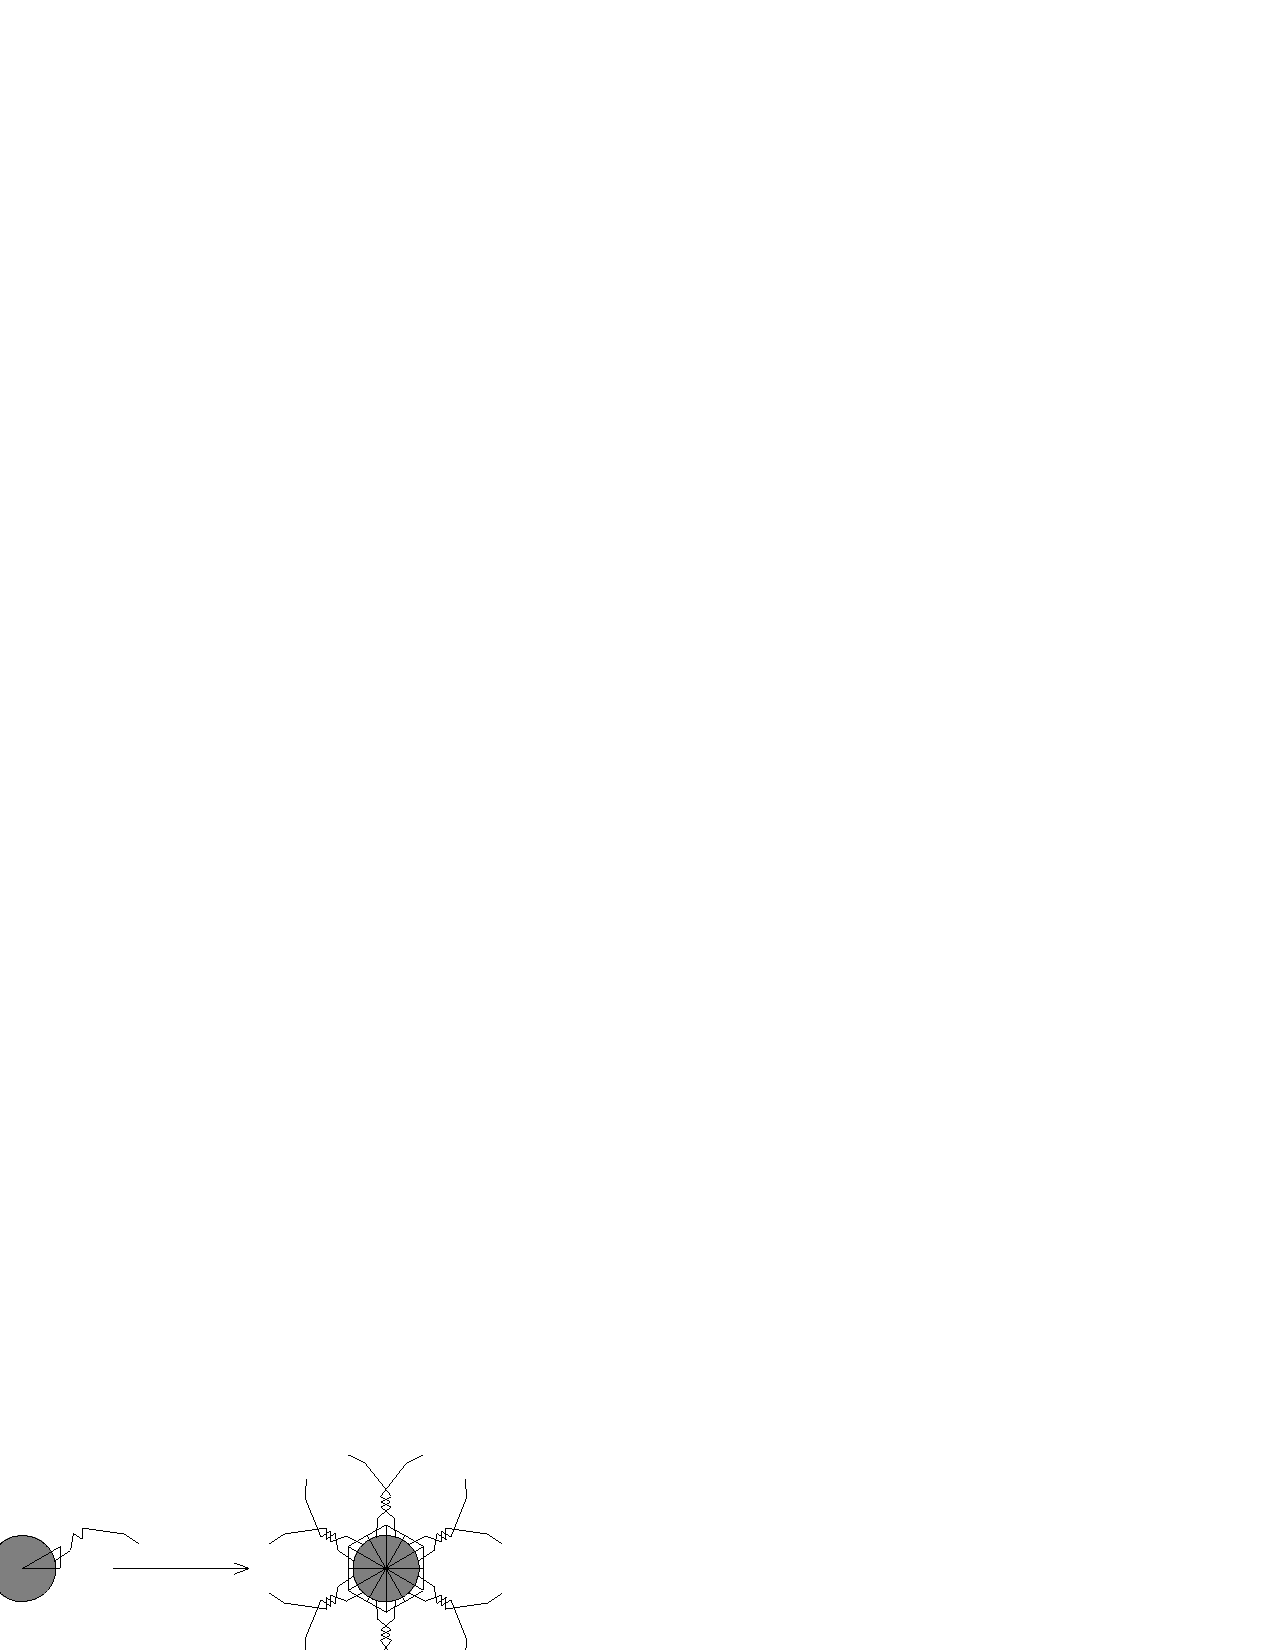
\includegraphics[width=0.45\textwidth]{diffuseSchreiberFig2}
\end{center}
\caption{
$\hp $ is the discrete transformation that relates the endpoint
of the cycle $\tp \in \tM$ to the endpoint of the corresponding
trajectory segment in $M$.
Eckmann\rf{LorentzDiff} Fig.~2. Remember to include
schreiberFig2.tex
    }
\label{schreiberFig2}
\end{figure}
%%%%%%%%%%%%%%%%%%%%%%%%%%%%%%%%%%%%%%%%%%%%%%%%%%%%%%%%%%%%%%%%%%%%%%%%



\section{Figure captions}

%%%%%%%%%%%%%%\item[Figure 1]%%%%%%%%%%%%%%%%%%%%%%%%%%%%%%%%%%%%%%%%%%
\begin{figure}
\begin{center}
\setlength{\unitlength}{15pt}
\begin{picture}(3,5.1)(1.5,1.5)
\put(5.15,3.336){\line(0,1){1.336}} \put(2.85,3.336){\line(0,1){1.336}}
\put(4,2.646){\line(5,3){1.15}}     \put(4,2.646){\line(-5,3){1.15}}
\put(4,5.354){\line(5,-3){1.15}}    \put(4,5.354){\line(-5,-3){1.15}}
\put(4,4){\line(5,3){1.15}}         \put(4,4){\line(1,0){1.15}}
\put(4,4){\circle{2}}        \put(6.3,4){\circle{2}} \put(1.7,4){\circle{2}}
\put(5.15,5.992){\circle{2}} \put(2.85,5.992){\circle{2}}
\put(5.15,2.008){\circle{2}} \put(2.85,2.008){\circle{2}}
\put(2.85,2.008){\line(0,-1){0.7}} \put(2.85,0.7){\line(0,1){0.4}}
\put(3.65,1.9){\line(0,-1){1.2}}   \put(4.35,1.9){\line(0,-1){1.2}}
\put(3,0.8){\vector(-1,0){0.15}}   \put(2.85,0.8){\vector(1,0){0.8}}
\put(4,0.8){\vector(-1,0){0.35}}   \put(4,0.8){\vector(1,0){0.35}}
\put(3.8,0.4){$w$} \put(3.1,0.4){1}
\end{picture}
\end{center}
\caption{
 A small portion of a triangular Lorentz gas. The whole set of scatterers
can be obtained by translating  the
%hexagonal
elementary cell indicated in the figure.
%The arrangement can also be tiled with images of the fundamental domain
%under the symmetry group of the hexagon.
    }
\label{schreiberFig0}
\end{figure}
%%%%%%%%%%%%%%%%%%%%%%%%%%%%%%%%%%%%%%%%%%%%%%%%%%%%%%%%%%%%%%%%%%%%%%%%

\begin{description}

\item[Figure 2]
 A portion of a chaotic trajectory with about 300 bounces is shown.
Although the particle is often trapped between neighboring disks
%one of the triangular enclosures
for several bounces, there are also
segment of the trajectory
which take the particle over a large distance with few bounces.

\item[Figure 3]
The upper row shows the case when the preceding
segment has been a long one,
the lower row the case when it has been a short one.
The arrows at the end points
indicate the sense of the next change of direction.
Due to the discrete symmetry of the triangular lattice,
all translated, rotated or reflected copies of each
situation shown are denoted by the same symbol.

\item[Figure 4]
The upper row shows the case when the preceding
segment has been a short one,
the lower row the case when it has been a long one.

 \item[Figure 5]
Shown are global orbits which reduce to fixed points in the fundamental
domain. Five of them (a,b,c,C,D) are not pruned for $w=0.3$,
the spacing shown here. The sixth (B) is an example of a pruned
cycle; it exists for a dilute Lorentz gas, because
for the dense Lorentz gas its trajectory is blocked by the center
disk. Both B and D denote turns by 120 degrees, but
D also changes the sense of rotation at each bounce.
\end{description}


%figurewithtex psfile texfile height (in cm) width (in cm) caption  (will be centered)
%\def\figurewithtex #1 #2 #3 #4 #5\cr{\null\ifundefined{fig#1}\global
%\advance\FIGUREcount by 1\NEWDEF fig,#1,{Fig.~\number\FIGUREcount}\fi
%\write16{ FIG \number\FIGUREcount: #1}
%{\goodbreak\figcenter=\hsize\relax
%\advance\figcenter by -#4truecm
%\divide\figcenter by 2
%\midinsert\vskip #3truecm\noindent\hskip\figcenter
%\special{psfile=#1}{\hskip\texpscorrection\input #2 }\vskip 0.8truecm\noindent \vbox{\eightpoint\noindent
%{\bf\fig(#1)}: #5}\endinsert}}
%\def\fig(#1){\ifundefined{fig#1}\global
%\advance\FIGUREcount by 1\NEWDEF fig,#1,{Fig.~\number\FIGUREcount}
%\fi

%%%%%%%%%%%%%%\item[Figure 2]%%%%%%%%%%%%%%%%%%%%%%%%%%%%%%%%%%%%%%%%%%
\begin{figure}
\begin{center}
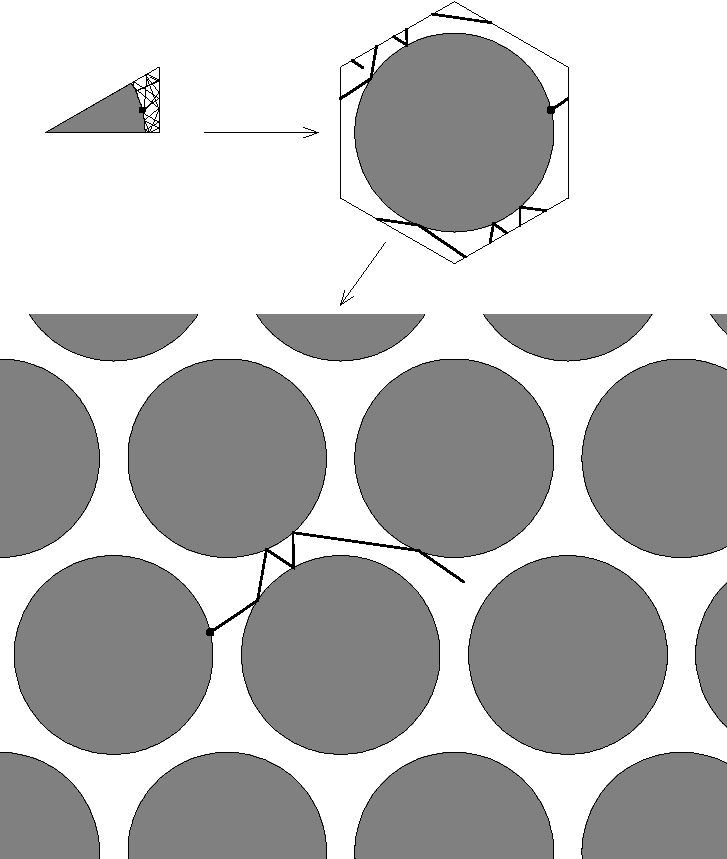
\includegraphics[width=0.45\textwidth]{diffuseSchreiberFig1}
\\
%\figurewithtex ../figs/diffuseSchreiberFig1.pdf ../diffuse/LorentzDiff/ps/fig1.tex 15 17
\end{center}
\caption{
Eckmann\rf{LorentzDiff} Fig.~1, from dif15.pdf. Remember to include
(misnamed) schreiberFig1.tex
    }
\label{schreiberFig1}
\end{figure}
%%%%%%%%%%%%%%%%%%%%%%%%%%%%%%%%%%%%%%%%%%%%%%%%%%%%%%%%%%%%%%%%%%%%%%%%

%%%%%%%%%%%%%%\item[Figure 4]%%%%%%%%%%%%%%%%%%%%%%%%%%%%%%%%%%%%%%%%%%
\begin{figure}
\begin{center}
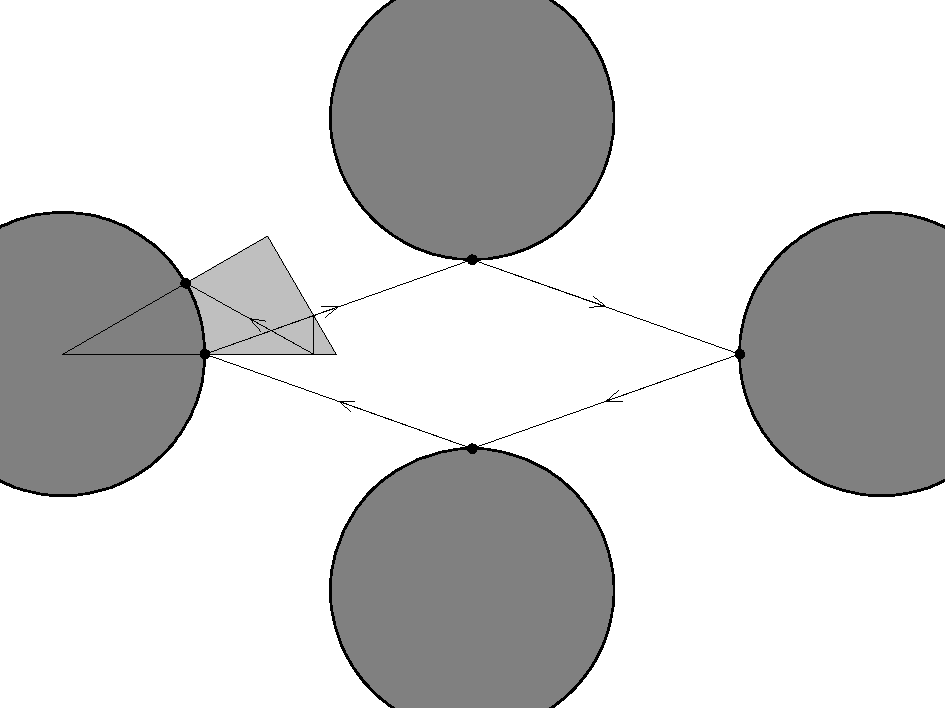
\includegraphics[width=0.45\textwidth]{diffuseSchreiberFig3}
\end{center}
\caption{
Eckmann\rf{LorentzDiff} Fig.~3. Remember to include
schreiberFig3.tex
    }
\label{schreiberFig3}
\end{figure}
%%%%%%%%%%%%%%%%%%%%%%%%%%%%%%%%%%%%%%%%%%%%%%%%%%%%%%%%%%%%%%%%%%%%%%%%


\section{Flotsam}

%%%%%%%%%%%%%%\item[Figure 4]%%%%%%%%%%%%%%%%%%%%%%%%%%%%%%%%%%%%%%%%%%
\begin{figure}
\begin{center}
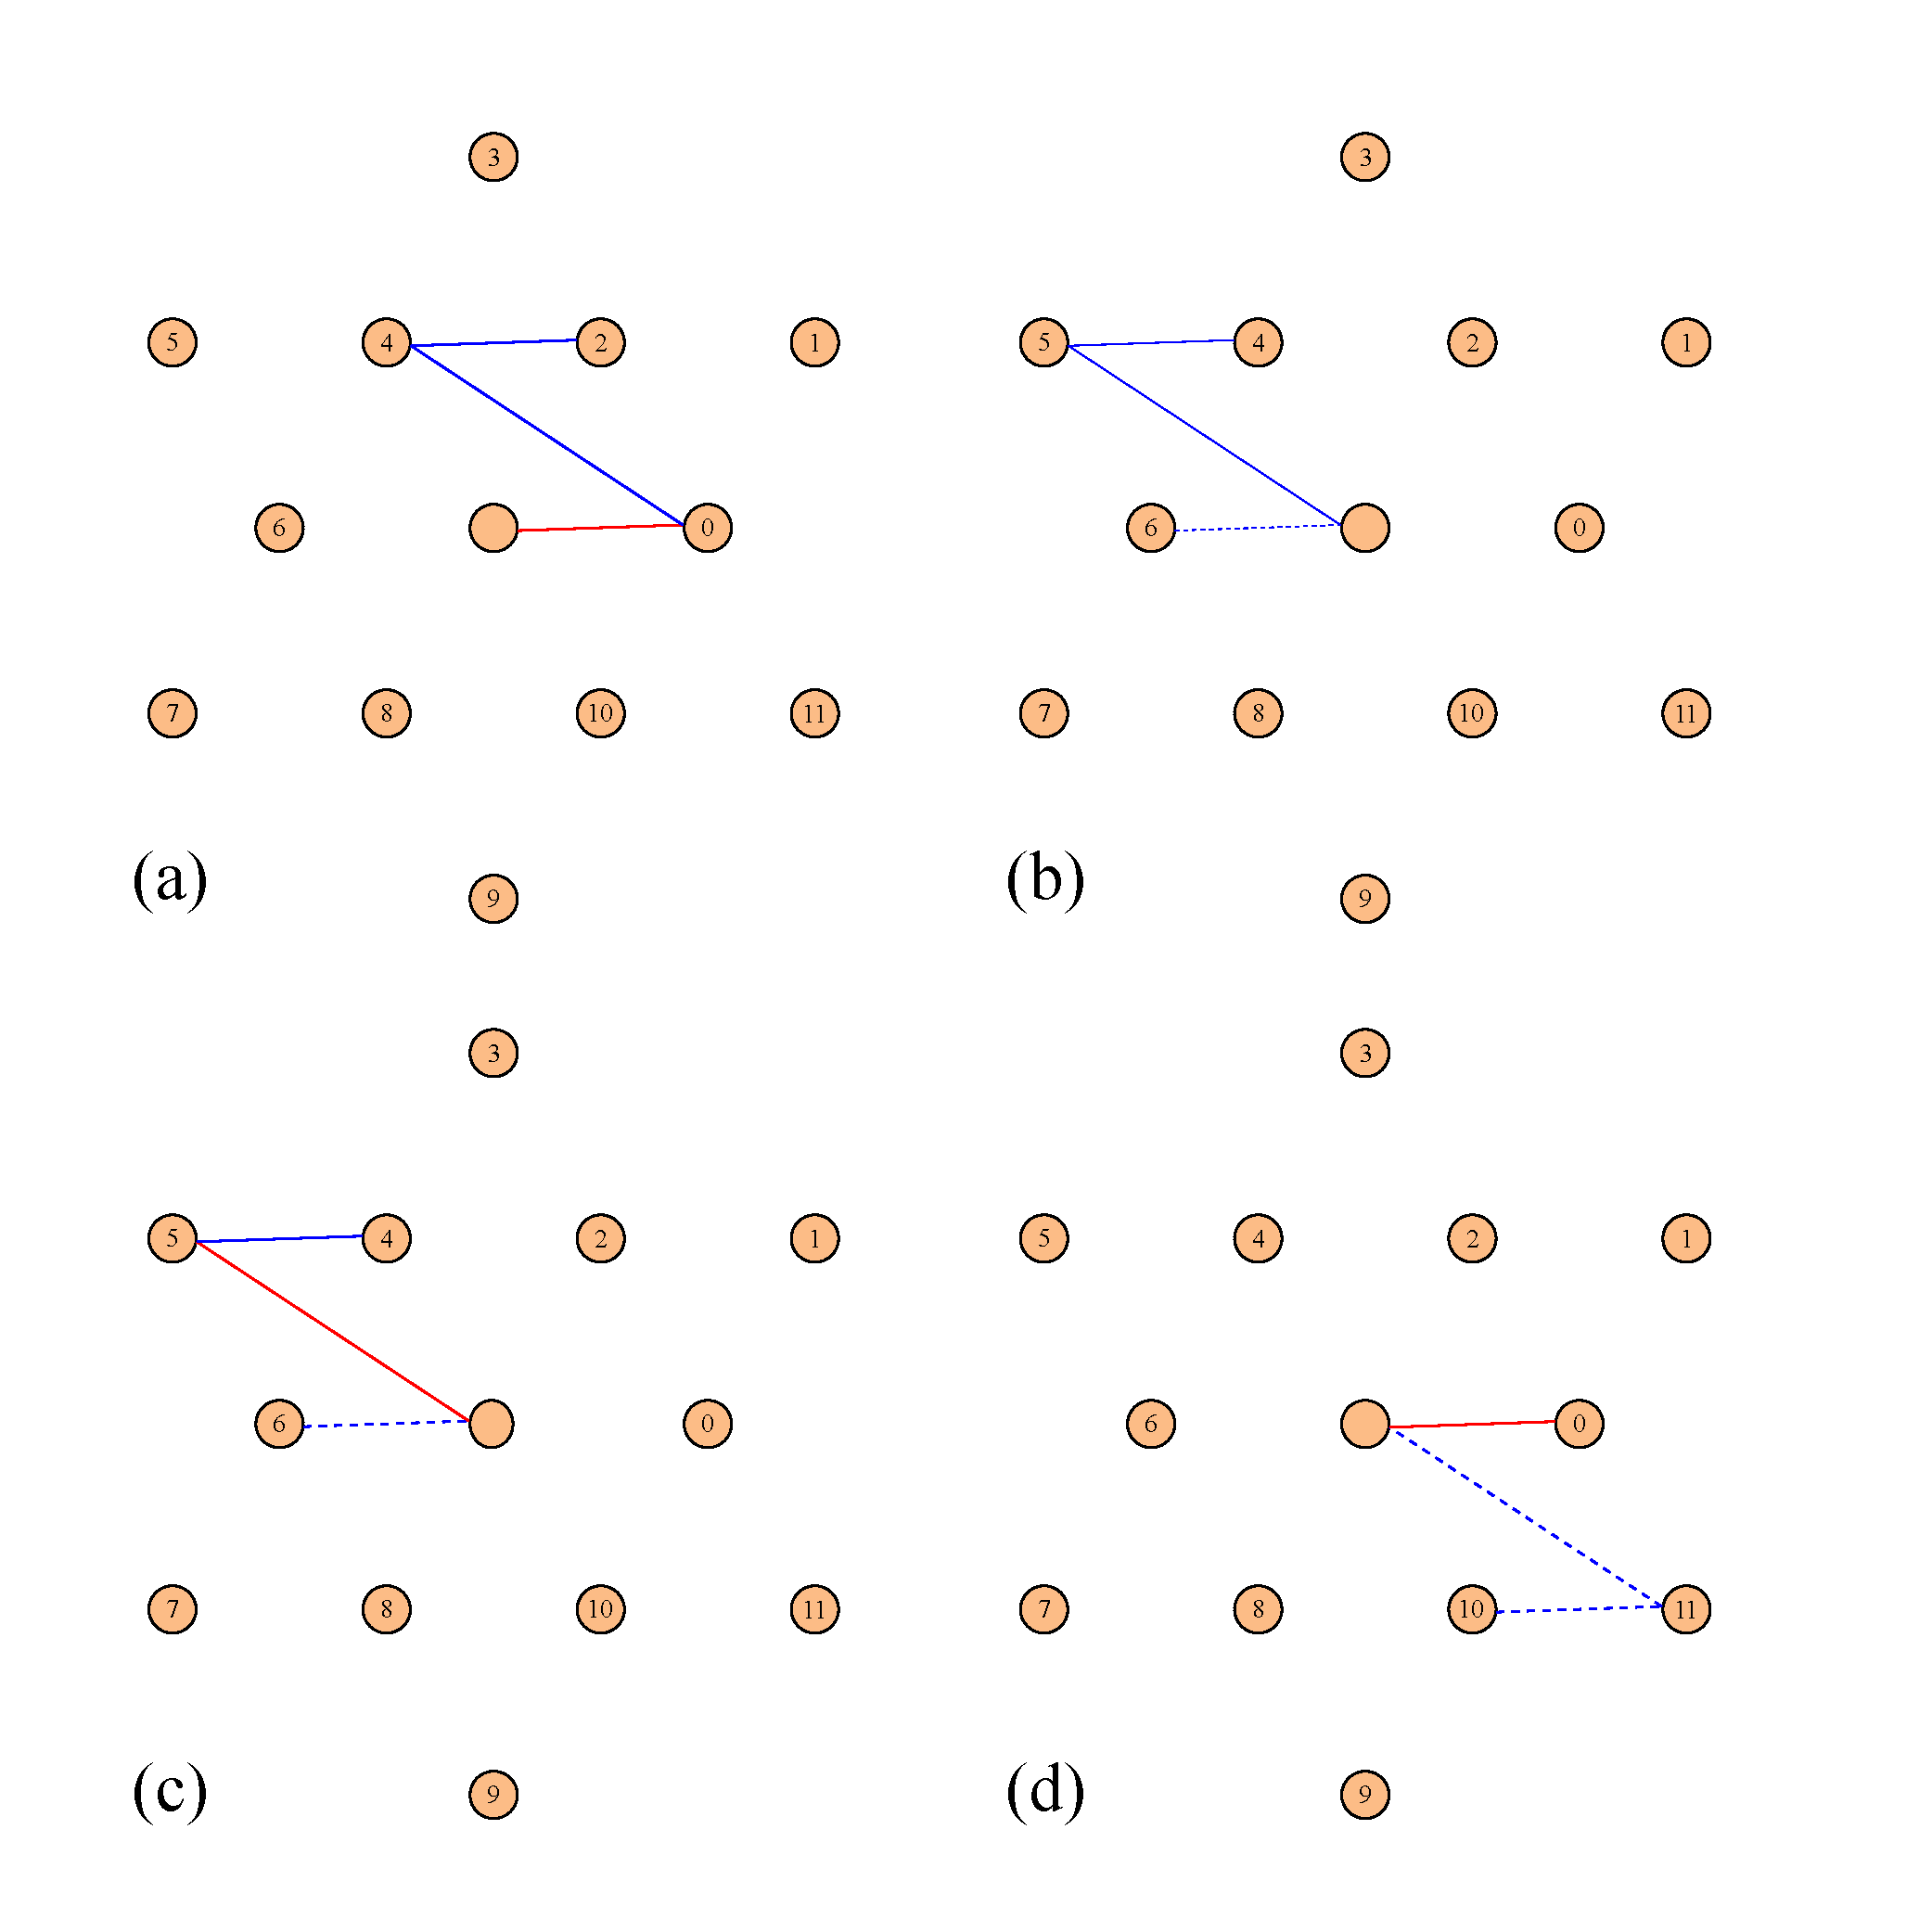
\includegraphics[width=1.0\textwidth]{diffuseDiskLabelsElCell_Orbits}
%(a) \includegraphics[width=0.35\textwidth]{diskLabelsElCell}
%~~~~(b) \includegraphics[width=0.35\textwidth]{diskLabelsElCell}
%\\[3.5ex]
%(c) \includegraphics[width=0.35\textwidth]{diskLabelsElCell}
%~~~(d) \includegraphics[width=0.35\textwidth]{diskLabelsElCell}
\end{center}
\caption{
Elementary cell symbolic dynamics, thin disks with  finite horizon
imposed by limiting jumps from the center cell to only short (even
labels) and long (odd labels) jumps.
(a) The first jump is a short one, from center disk to disk 0.
(b) Reduction to the elementary cell using the translation group:
the array is shifted so the current disk is a now the
center, all neighbors are relabelled, and the shift $n_1$
is stored.
(c) The second jump is a long one to disk 5.
(d) The array is shifted so the current disk is a now the center, and the
shift $n_2$ is stored. The prime 2-cycle \cycle{05} (\rpo; running mode),
of period $\period{05}=\zeit_1+\zeit_2$ and shift $n_{05} = n_1+n_2$
repeats this sequence forever. All 12 rotations (full \Dn{6} group) of
this cycle are distinct under translations.
    }
\label{diskLabelsElCell}
\end{figure}
%%%%%%%%%%%%%%%%%%%%%%%%%%%%%%%%%%%%%%%%%%%%%%%%%%%%%%%%%%%%%%%%%%%%%%%%

% Table generated by Excel2LaTeX from sheet 'Sheet1'
\begin{table}[htbp]
  \centering
  \caption{cycle 2 periodic orbits}
    \begin{tabular}{|r|r|r|r|}
    \hline
    \multicolumn{1}{|c|}{lambda} & \multicolumn{1}{|c|}{tp} & floquet & shift \\\hline
    4.539722 & 0.600000 & 2.52144304 & (0,0) \\
    4.539722 & 0.600000 & 2.52144304 & (0,0) \\
    4.539722 & 0.600000 & 2.52144304 & (0,0) \\
    23.530813 & 2.678876 & 1.17896877 & (0,-1) \\
    23.530816 & 2.678876 & 1.17896882 & (-1,1) \\
    23.530817 & 2.678876 & 1.17896884 & (1,0) \\
    23.530817 & 2.678876 & 1.17896884 & (-1,0) \\
    23.530818 & 2.678876 & 1.17896885 & (1,0) \\
    23.530821 & 2.678876 & 1.17896889 & (0,1) \\
    23.530821 & 2.678876 & 1.1789689 & (0,1) \\
    23.530821 & 2.678876 & 1.1789689 & (1,-1) \\
    23.530821 & 2.678876 & 1.1789689 & (0,-1) \\
    23.530822 & 2.678876 & 1.17896891 & (1,-1) \\
    23.530823 & 2.678876 & 1.17896893 & (-1,1) \\
    23.530824 & 2.678876 & 1.17896894 & (-1,0) \\
    33.580486 & 3.967434 & 0.88569725 & (0,0) \\
    33.580486 & 3.967434 & 0.88569725 & (0,0) \\
    33.580486 & 3.967434 & 0.88569725 & (0,0) \\
    105.577475 & 4.927474 & 0.9456052 & (-1,-1) \\
    105.577492 & 4.927474 & 0.94560523 & (-2,1) \\
    105.577500 & 4.927474 & 0.94560525 & (1,1) \\
    105.577512 & 4.927474 & 0.94560527 & (1,-2) \\
    105.577518 & 4.927474 & 0.94560528 & (-1,2) \\
    105.577518 & 4.927474 & 0.94560528 & (-1,1) \\
    \hline
    \end{tabular}%
  \label{tab:length2withfloquet}%
\end{table}%



\begin{description}

\item[2014-05-12 Predrag to Tingnan]
I created a sketch of \reffig{diskLabelsElCell} which should explain step
by step how one goes from absolute labeling of disks on the infinite
hexagonal lattice to the translation-quotiented elementary cell, step by
step. Please generate this in Matlab, but with resulting figures as here
(small disks, no axes, etc.). What made the file so big (my
\texttt{*.svg} is 10 times smaller) were the fat red circles, which were
raster rather than vector graphics - replace them in Matlab code with a
thin line circle, hopefully that will be drawn in the vector format, so I
do not have to manually clean them up in \texttt{Inkscape}.

\item[2014-05-20 Predrag]
Replaced \reffig{diskLabelsElCell} by \reffig{diskDirectionsElCell},
labeling the translation vectors connecting the center of the current
disk to the center of the next disk.

\end{description}


%%%%%%%%%%%%%%%%%%%%%%%%%%%%%%%%%%%%%%%%%%%%%%%%%%%%%%%%%%%%%
\newpage
%\bibliographystyle{../inputs/adkPCphysrev} % PC trying Phys Rev style,
                                            % but with article titles
%\addcontentsline{toc}{chapter}{Bibliography}
\printbibliography[title={References}] %, type=online]
%\bibliography{../bibtex/siminos}
%%%%%%%%%%%%%%%%%%%%%%%%%%%%%%%%%%%%%%%%%%%%%%%%%%%%%%%%%%%%%

% GitHub cvitanov/reducesymm/tingnan/spaceGroups.tex

% Predrag                                       2014-07-14
	
\chapter{Notes on space groups}
\label{c-spaceGroups}




\begin{description}

\item[2014-07-14 Predrag]
Separated out here our notes on condensed matter theorists'
standard version of space groups (the one we are too lazy to learn)

\item[2014-04-18 Predrag]
Dresselhaus \etal\ textbook\rf{Dresselhaus07}
(\HREF{http://chaosbook.org/library/Dresselhaus07.pdf}{click here})
is good on discrete
and space (but not continuous) groups.
The MIT~course~6.734
\HREF{http://stuff.mit.edu/afs/athena/course/6/6.734j/www/group-full02.pdf}
{online version} contains much of the same material.

Chapter {\em 9. Space Groups in Real Space} is quite clear on matrix
representation of space groups. The translation group $T$ is a normal
subgroup of \Group\ and defines the Bravais lattice. The cosets by
translation $T$ (set all all group elements obtained by all translations)
form a factor group $\Group/T$, isomorphic to the point group $g$
(rotations). All irreducible representations of \Group\ can be compounded
from irreducible representations of $g$ and $T$.

Section {\em 9.3 Two-Dimensional Space Groups}: In the international
crystallographic notation, our hexagonal lattice \#17 is called $p6mm$,
with point group $6mm$.
\beq
\Group = \{
E, C_6^+, C_6^-, C_3^+, C_3^-, C_2,
\sigma_{d1}, \sigma_{d2}, \sigma_{d3},
\sigma_{v1},\sigma_{v2}, \sigma_{v3}
\}
\ee{D12generators}
Prefix $p$ indicates that the unit cell is primitive (not centered). This
is a simple or {\em symmorphic} group, which makes calculations easier.
The Bravais lattice is two equilateral triangles, not sure how to relate
it to our hexagonal `elementary cell'? A Brilloun zone? Bravais `unit cell'
is illustrated in Fig.~E.2. ChaosBook `Fundamental
domain' makes an appearance in Fig.~10.2.

The main trick in quantum-mechanical calculations is to go to the
\emph{reciprocal} space (see Fig.~E.2), in our case with the full
$\Gamma$ point, $k=0$, wave vector symmetry (see Table~10.1), and `Large
Representations'. This is something we have not tried in deriving the
trace formula for deterministic diffusion.

Sect. {\em 10.5 Characters for the Equivalence Representation} look
like those for the point group, sort of. We should probably work
out problems 10.1 and 10.2.

\item[2014-04-26 Predrag] We should read Chapter 7 of Gaspard\rf{PG97}.
Kimberly and I both have a hard copy. Gaspard discusses irreps of
the translation group in some detail.

\item[2014-04-26 Predrag]
I'm quite convinced that this problem is a solved problem, we just have
to understand how characters are used to project irreps of space groups.
One has to go to the reciprocal lattice, and utilize utilize the concept
of the `star'. All physical chemists and crystallographers know how to do
this - we just need to be good students and read the stuff. Our case is
the most symmetric, $p6mm$ lattice - it is surely worked out in some
paper in a way that we can understand. They call our `fundamental domain'
the `motif' or the `asymmetric unit'.

I found projects in \HREF{http://www-f1.ijs.si/~ziherl/SF.html} {this
course} easy to read, especially Toma\v{z} \v{C}endak, who reviews the
space groups theory in a pretty simple way, and Zavadlav has very pretty
wallpaper groups illustrations. Ziherl recommends Elliott and  Dawber,
{\em Symmetry in Physics}\rf{ELLIOTT}.

Joseph Sidighi likes Cotton\rf{Cotton08} {\em Chemical applications of
group theory}, which has no characters for space groups, but a very
pretty discussion of their geometry in Chapt.~11. Cotton was ``the most
influential inorganic chemist to ever have lived.''

If we succeed in factorization, this would merit a publication.
It is OK if you do not succeed in factorization - I have failed myself, so
who am I to cast the first stone:)

\item[2014-05-05 Tingnan] My numbers of elementary cell prime cycles,
Lyapunov exponents and diffusion coefficients are listed and compared
to the Schreiber calculation in \reftab{TCELL1}. I still have the problem
for the convergence of diffusion coefficients. Did we miss a factor of 2
somewhere?

\item[2014-05-28 Tingnan] I got it!

I see the trouble more clearly as indicated in the previous blogs: The
averaging over the space group (a point group action followed by a
translation). I think in Pavel's approach we still needs to worry
because his three group actions do not commute with each other?

Let us speculate a bit about the group actions in the lattice group. We
will use the same notation as in Dresselhaus \etal\
textbook\rf{Dresselhaus07},
\[
	\mathbf{a} = \{R_g\vert\tau\}
\,
\]
where $g$ is an element of the point group and $\tau$ is a translation.

%A potentially useful commutation relation is posted here (9.15):
%\[	\{R_g\vert\tau\}\{\epsilon\vert\tau\}\{R_g\vert\tau\}^{-1} = \{\epsilon\vert R_gt\}
%\]

Since our group is $p6mm$ and is symmorphic, the irreducible representation
of the group (of the wave vector) is simple (10.35),
\[
D_{k}^{\Gamma_{i}}(\{R_{g}\vert\mathbf{R}_{n}\})=e^{i\mathbf{k\cdot R}_{n}}D^{\Gamma_{i}}(R_{g})
\,
\]
where $D^{\Gamma_{i}}(R_{g})$ is the irreps of the point group $C_{6v}$,
which can be readily found (\HREF{http://www.cryst.ehu.es}{click here}).

\item[2014-06-03] Finally I got Gaspard's book from the GIL service. Here
are updates on reciprocal lattice.

Suppose we have $M$ dimensional phase space flow $f^{t}(\mathbf{X})$
with $L<M$ position coordinates. The equation of motion is invariant
under a space group $G$. Let us first examine the translation subgroup
$T$ of $G$.

With a proper choice of {\Poincare} section $\mathcal{P}$, the flow
$f^{t}(\mathbf{X})$ can be expressed as a suspended flow $F^{t}(\mathbf{x},\tau,\mathbf{l})$
(Gaspard 7.8), where $\mathbf{x}\in\mathcal{P}$ is on the section,
$\tau\in[0,T(\mathbf{x}))$ the time interval before first return,
and $\mathbf{l}$ a spatial vector denotes the center of the element
cell the current point belongs to. The flow is controlled by a set
of mappings:

\[
\begin{cases}
\mathbf{x}_{n+1}=\phi(\mathbf{x}_{n}) & \mathbf{x\in\mathcal{P}}\\
t_{n+1}=t_{n}+T(\mathbf{x}_{n})\\
\mathbf{l}_{n+1}=\mathbf{l}_{n}+a(\mathbf{x}_{n}) & a(\mathbf{x}_{n})\in\mathcal{L}
\end{cases},
\]
where we denote the Bravais lattice $\mathcal{L}$. We can relate
the mappings with the flow:
\begin{align*}
F^{t}(\mathbf{x},\tau,\mathbf{l}) & =\left\{ \phi^{n}\mathbf{x},\tau+t-\sum_{j=0}^{n-1}T(\phi^{j}\mathbf{x}),\mathbf{l}+\sum_{j=0}^{n-1}a(\phi^{j}\mathbf{x})\right\} ,\\
 & \qquad\mathrm{for}\qquad0\leq\tau+t-\sum_{j=0}^{n-1}T(\phi^{j}\mathbf{x})<T(\phi^{n}\mathbf{x}).
\end{align*}


We can define invariant measures based on the special coordinates
$(\mathbf{x},\tau,\mathbf{l})$ (Gaspard 7.20-7.21):
\begin{align*}
\left\langle A(\mathbf{X})\right\rangle  & =\sum_{\mathbf{l}\in\mathcal{L}}\int\mu(d\mathbf{x}d\tau)A(\mathbf{x},\tau,\mathbf{l})\\
 & =\sum_{\mathbf{l}\in\mathcal{L}}\frac{1}{\vert\mathcal{P}\vert}\int_{\mathcal{P}}d\mathbf{x}\int_{0}^{T(\mathbf{x})}\frac{d\tau}{\left\langle T\right\rangle _{\nu}}A(\mathbf{x},\tau,\mathbf{l})\\
 & =\sum_{\mathbf{l}\in\mathcal{L}}\frac{1}{\left\langle T\right\rangle _{\nu}}\left\langle \int_{0}^{T(\mathbf{x})}d\tau A(\mathbf{x},\tau,\mathbf{l})\right\rangle _{\nu}
\end{align*}
where the subscript $\nu$ denotes integration over the volume of
the {\Poincare} section.

Now with some quantities defined let us proceed to the fourier transforms
of the quantities we are interested. Define the projection operators by
\begin{align*}
\hat{E}_{\mathbf{k}} & =\sum_{\mathbf{R}_{n}}e^{-i\mathbf{k}\cdot\mathbf{R}_{n}}\hat{P}_{\{\varepsilon\vert\mathbf{R}_{n}\}},
\end{align*}
in terms of spatial translation operators
\[
\hat{P}_{\{\varepsilon\vert\mathbf{R}_{n}\}}\phi(\mathbf{r})=\phi(\mathbf{r}+\mathbf{R}_{n}),
\]
with $\mathbf{R}_{n}$ is the Bravais lattice vector, and $\mathbf{k}\in\mathcal{B}$,
the first Brillouin zone. For an infinite lattice $\mathbf{k}$ is
continuous. We first needs to check and orthogonality and completeness
of the projection operators (Gaspard 7.30-7.32) :
\begin{align*}
\hat{E}_{\mathbf{k}}\hat{E}_{\mathbf{k^{\prime}}} & =\sum_{\mathbf{R}_{n}}e^{-i\mathbf{k}\cdot\mathbf{R}_{n}}\hat{P}_{\{\varepsilon\vert\mathbf{R}_{n}\}}\sum_{\mathbf{R}_{m}}e^{-i\mathbf{k^{\prime}}\cdot\mathbf{R}_{m}}\hat{P}_{\{\varepsilon\vert\mathbf{R}_{m}\}}\\
 & =\sum_{\mathbf{R}_{n}\mathbf{R}_{m}}e^{-i(\mathbf{k}\cdot\mathbf{R}_{n}+\mathbf{k}^{\prime}\cdot\mathbf{R}_{m})}\hat{P}_{\{\varepsilon\vert\mathbf{R}_{n}+\mathbf{R}_{m}\}}\\
 & =\sum_{\mathbf{R}_{m}}\sum_{\mathbf{R}_{l}}e^{-i(\mathbf{k}\cdot(\mathbf{R}_{l}-\mathbf{R}_{m})+\mathbf{k}^{\prime}\cdot\mathbf{R}_{m})}\hat{P}_{\{\varepsilon\vert\mathbf{R}_{l}\}}\\
 & =\sum_{\mathbf{R}_{m}}e^{-i(\mathbf{k}^{\prime}-\mathbf{k})\cdot\mathbf{R}_{m}}\sum_{\mathbf{R}_{l}}e^{-i\mathbf{k}\cdot\mathbf{R}_{l}}\hat{P}_{\{\varepsilon\vert\mathbf{R}_{l}\}}\\
 & =\hat{E}_{\mathbf{k}}\sum_{\mathbf{R}_{m}}e^{-i(\mathbf{k}^{\prime}-\mathbf{k})\cdot\mathbf{R}_{m}}\\
 & =\hat{E}_{\mathbf{k}}\vert\mathcal{B}\vert\delta(\mathbf{k}^{\prime}-\mathbf{k})
\end{align*}

\begin{align*}
\frac{1}{\vert\mathcal{B}\vert}\int_{\mathcal{B}}\hat{E}_{\mathbf{k}}d\mathbf{k} & =\frac{1}{\vert\mathcal{B}\vert}\sum_{\mathbf{R}_{n}}\hat{P}_{\{\varepsilon\vert\mathbf{R}_{n}\}}\int_{\mathcal{B}}e^{-i\mathbf{k}\cdot\mathbf{R}_{n}}d\mathbf{k}\\
 & =\frac{1}{\vert\mathcal{B}\vert}\sum_{\mathbf{R}_{n}}\hat{P}_{\{\varepsilon\vert\mathbf{R}_{n}\}}\vert\mathcal{B}\vert\delta_{\mathbf{R}_{n},0}\\
 & =\hat{P}_{\{\varepsilon\vert0\}}\\
 & =\hat{I}.
\end{align*}

to be continued.

\item[2016-05-07 Predrag]                                       \toCB
Reading on
`fundamental domain',
`chamber',
`M\"obius triangle',
`Voronoi cell',
`primitive cell',
`Wigner-Seitz cell',
`orbifold',
`signature',
`reflection group',
`Coxeter group',
`triangle group',
`bisected hexagonal tiling',
`',
$\cdots$

% https://en.wikipedia.org/wiki/Fundamental_domain
%
Given a topological space and a group acting on it, the images of a
single point under the group action form an \emph{orbit} of the action. A
\emph{fundamental domain} (also called fundamental region) is a subset of
the space which \emph{contains exactly one point} from each of these
orbits.
Typically, a fundamental domain is required to be a connected subset with
some restrictions on its boundary, for example, smooth or polyhedral. The
images of a chosen fundamental domain under the group action then tile
the space. One general construction of fundamental domains uses Voronoi
cells.

Example: for reflection in a hyperplane: an orbit is either a set of 2
points, one on each side of the hyperplane, or a single point in the
hyperplane; the fundamental domain is a half-space bounded by that
hyperplane.

Example: for discrete translational symmetry in three directions: the
orbits are translates of the lattice; the fundamental domain is a
\emph{primitive cell} which is e.g. a parallelepiped, or a
\emph{Wigner-Seitz cell}, also called \emph{Voronoi cell/diagram}. In the
case of translational symmetry combined with other symmetries, the
fundamental domain is part of the primitive cell. For example, for
wallpaper groups the fundamental domain is a factor 1, 2, 3, 4, 6, 8, or
12 smaller than the primitive cell.

    If one identifies equivalent points of a symmetric pattern, the
    resulting space is called an orbifold. In Thurston's
    \HREF{http://www.geom.uiuc.edu/docs/doyle/mpls/handouts/handouts.html}
    {original definition}, an orbifold is a quotient of a 2\dmn\ space
    with a finite discrete group. Conway has generalized this to 3- and
    4-dimensions\rf{CBG16}, but I have not found anything about higher
    dimensions.

In string theory, the word ``orbifold" has a slightly new meaning.

% https://en.wikipedia.org/wiki/Orbifold
%
For mathematicians, an orbifold is a generalization of the notion of
manifold that allows the presence of the points whose neighborhood is
diffeomorphic to a quotient of $\reals^n$ by a \emph{finite} group, i.e.
$\reals^n/\Group$.

In physics, the notion of an orbifold usually describes an object that
can be globally written as an orbit space $M/\Group$ where $M$ is a manifold
(or a theory), and $G$ is a group of its isometries (or symmetries) -- not
necessarily all of them.

A theory defined on an orbifold becomes singular near the fixed points of
$\Group$.

When the orbifold group $\Group$ is a discrete group, and it has fixed
points, then these usually have conical singularities, because
$\reals^n/Z_k$ has such a singularity at the fixed point of $Z_k$.

\item[2016-05-07 Predrag] From Tim Perutz
\HREF{https://www.ma.utexas.edu/smmg/archive/2012/Perutz/PerutzSlides.pdf}
{slides}, a very brief glimpse of Conway, Burgiel and
Goodman-Strauss\rf{CBG16}:

Symmetry operations that leave a plane pattern unchanged:
\begin{description}
  \item[Rotation] rotate by an angle about a center.
  \item[Reflection] mirror reflection across a line
  \item[Glide] reflect across a line, then translate in the
      direction of that line. Think: footprints!
\end{description}
A sequence of two reflections can be a rotation.

Patterns are classified by their \emph{orbifolds} and \emph{signatures}.
In our case, the pattern is a hexagonal tiling, and orbifold is the
fundamental domain. Thurston's signature in that case is $*632$; see
p.~310 in Thurston's \HREF{http://library.msri.org/books/gt3m/PDF/13.pdf}
{notes}.

The \emph{orbifold} of a pattern is the geometric object we get from the
plane when we regard two points to be equal if they are related by
a symmetry of the pattern.

The \emph{signature} of an orbifold describes the features you would need
to add to make it.

$*$ means you punch a hole, so as to make a boundary, etc - see the slides.
It is far from obvious, and it works only in $2D$.

Centers of rotation give sharp points like cones.

% https://en.wikipedia.org/wiki/Reflection_group
%
A \emph{reflection group} is a discrete group which is generated by a set of
reflections of a finite-dimensional Euclidean space. The symmetry group
of a regular polytope or of a tiling of the Euclidean space by congruent
copies of a regular polytope is necessarily a reflection group.
Reflection groups also include Weyl groups and crystallographic Coxeter
groups.

A finite reflection group is a subgroup of the general linear group of E
which is generated by a set of orthogonal reflections across hyperplanes
passing through the origin.

In two dimensions, the finite reflection groups are the dihedral groups,
which are generated by reflection in two lines that form an angle of
$2\pi/n$ and correspond to the Coxeter diagram $I_2(n)$.

Infinite reflection groups include the frieze groups and the wallpaper
groups (our example is is $*632$).

H.S.M. Coxeter\rf{Coxeter34,Coxeter35}: The reflections in the faces of a
fixed fundamental ``chamber'' (our ``fundamental domain'') are generators
$r_i$ of a reflection group of order 2. All relations between them follow
from
\[
    (r_i r_j)^{c_{ij}}=1
\]
expressing the fact that the product of the reflections $r_i$  and $r_j$
in two hyperplanes $H_i$  and $H_j$ meeting at an angle $\pi/c_{ij}$ is a
rotation by the angle $2\pi/c_{ij}$ fixing the subspace $H_i \cap H_j$ of
codimension 2.

% https://en.wikipedia.org/w/index.php?title=Triangle_group&action=edit
%
A \emph{triangle group} is a group that can be realized geometrically by
sequences of reflections across the sides of a triangle. Each triangle
group is the symmetry group of a tiling of the Euclidean plane by
congruent triangles, a fundamental domain for the action
 (the triangle defined by the lines of reflection), called a
M\"obius triangle.
Thus a triangle group is a reflection group that admits a  group presentation
\[
\Delta(l,m,n) = \langle a,b,c
\mid a^{2} =  b^{2} = c^{2} = (ab)^{l} = (bc)^{n} = (ca)^{m} =  1 \rangle
\,.
\]
An abstract group with this presentation is a Coxeter group with three
generators.

The triangle group is the infinite symmetry group of a certain
tessellation (or tiling) of the Euclidean plane by triangles. Up to
permutations, the triple (l, m, n) is one of the triples (2,3,6),
(2,4,4), (3,3,3). The corresponding triangle groups are instances of
wallpaper groups. Our case is the ``bisected hexagonal tiling'' (2,3,6).

% https://people.math.osu.edu/davis.12/papers/lectures%20on%20orbifolds.pdf
%
{\em reflectofolds}: orbifolds coming from groups generated by reflections.

% https://www.ime.usp.br/~gorodski/ps/orbit-spaces-revision2016.pdf
%
A Riemannian orbifold is called a Coxeter orbifold if all local groups
are Coxeter groups acting as reflection groups on the corresponding
tangent spaces (Davis\rf{Davis08,Davis10} calls them reflectofolds).






\end{description}

% GitHub cvitanov/reducesymm/tingnan/3gener.tex

% Predrag                                       2014-04-18
	
\chapter{3 generator tiling}
\label{c-3gener}

% \item[2014-07-14 Predrag]
My intuition is that the symbolic dynamics is robust under varying
the disk spacing $w$ - for sufficiently large $w$ there is no pruning, and all
of our short/long hop orbits are allowed. As $w$ decreases, some of them get pruned,
but symbolic dynamics should not change - if you label disks, it labels the same
sequence of disk visitations (I do not how to prove this, so I might be wrong.)

\refFig{fig:cycle026A} is a nice illustration; there are
many equivalent sequences of three generators $\{s,\ell,f\}$ and
the problem is that of determining isomorphisms between deterministic
finite automata. Here we show how to `quotient' equivalent
substrings.

We know that on the elementary
cell level there are only 11 (or 12 -  one isomorphism) symbols, so maybe
we can figure how to uniquely relabel the $\{s,\ell,f\}$ itineraries in
terms of such set.


%%%%%%%%%%%%%%\item[Figure ?]%%%%%%%%%%%%%%%%%%%%%%%%%%%%%%%%%%%%%%%%%%
\begin{figure}
\begin{center}
(a) 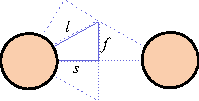
\includegraphics[width=0.45\textwidth]{diffuse7diskFundDflips}
(b) 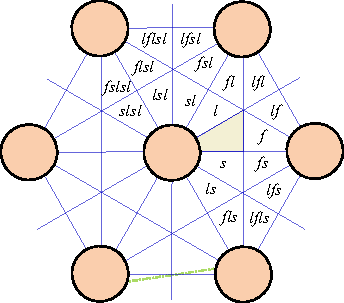
\includegraphics[width=0.45\textwidth]{diffuse7diskFundDtiles}
\end{center}
\caption{
(a) The three generators of tiling of the plane by a fundamental domain:
two generators of \Dn{12} tiling, reflection $s$ across the short
disk-disk separation, reflection  $\ell$  across the long disk-disk
separation;
and
a translation generator $f$ that pivots (`flips') a disk center to disk
center by flip across the symmetry line normal to the short disk-disk
separation.
(5) Tiling of the 7-disk by copies of the fundamental domain, labelled
by a (not unique) sequence of the three generators
$\{s,\ell,f\}$, chosen so that each sequence contain one and only on
    disk-to-disk pivot $f$.
        }
\label{7diskFundDflipsA}
\end{figure}
%%%%%%%%%%%%%%\item[Figure 4]%%%%%%%%%%%%%%%%%%%%%%%%%%%%%%%%%%%%%%%%%%

% \item[2014-06-02, 2014-06-08 Predrag]
\refFig{7diskFundDflipsA}\,(a) illustrates the three generators
\beq
    \{s,\ell,f\}
\,.
\ee{3gener}
In the international
crystallographic notation, our hexagonal lattice is called $p6mm$,
with point group $6mm$,
where
prefix $p$ indicates that the unit cell is primitive (not centered),
\beq
\Group = \{
e, C_6^+, C_6^-, C_3^+, C_3^-, C_2,
\sigma_{d1}, \sigma_{d2}, \sigma_{d3},
\sigma_{v1},\sigma_{v2}, \sigma_{v3}
\}
\,,
\ee{D12generatorsA}
with $s=\sigma_{d}$ the reflection across the
short disk-disk separation, and $\ell=\sigma_{v}$ reflection across the
long disk-disk separation generators of \Dn{12}. The entire space group
is then generated by adding a disk-to-disk generator $f$ that pivots a
disk center to disk center by flip across the symmetry line normal to the
short disk-disk separation.
We find it convenient to define $C$ as the generator of cyclic rotations
by $\pi/3$,
\[
\ell s = C_6^- = C
\,,\quad
C^6 = e
\,;\qquad
s \ell =  C_6^+
\,,\qquad
s  =  C_6^+ \ell
\,.
\]
There are two short paths from disk to disk: $f$, which keeps the sense
of orientation, and $sf=fs$ which changes it.

\begin{figure}
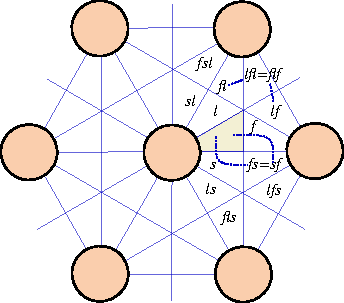
\includegraphics[width=\textwidth]{diffuse7diskFundDtilesEquiv}
\caption{Shortest equivalent sequences.}
\label{fig:symbolEquivA}
\end{figure}


The (hopefully complete) list of the
equivalence relations, \ie, different sequences of operations reaching
the same copy of the fundamental domain is:
\beq
s s = e
\,,\quad
\ell \ell = e
\,,\quad
f f = e
\,,\quad
C^6 = e
\,;\qquad
f s = s f
\,,\quad
f \ell f=\ell f \ell
\,.
\ee{3generEquiv}
The two flips $f s = s f$ act at $90^0$ and hence commute.
As shown in \reffig{fig:symbolEquivA}, $f\ell f$ and $\ell f \ell$
map the fundamental domain to the same copy. Finally, $C^6 = e$ ensures
that the tiling is hexagonal.

Our task is to generate all distinct
itineraries from $\{s,\ell,f\}$, by pre-pending a letter to a given sequence.
Repeats of the 3 letters are not allowed (so tree of admissible sequences
is binary), and neither is the sixth repeat of the
rotation $C$. The remaining two equivalence relations we impose by
crossing out any itinerary that contains block $f s$ or block $f\ell f$.
Prohibition of the block $f s$ implies that $s$ is always followed by $\ell$,
\ie, we can replace the $s$ at last position in an itinerary by
$ s \to \ell s = C$,
with $\ell C$ prohibited in the next step.
We start with the three starting letters $\{s,\ell,f\}$, and generate the admissible
itineraries tree as follows:
\bea
&s & \quad\quad \ell \quad\qquad f
    \continue
& C & \quad s \ell, f \ell \qquad s f , \ell f
    \continue
&s C, f C & \quad
    C \ell; s f \ell , \ell f \ell \qquad
        C f ; s \ell f
    \label{3generTree}\\
&C^2; s f C, \ell f C & \quad
    s C \ell, f C \ell; C f \ell ;  s \ell f \ell  \qquad
       s C f, f C f  ; C \ell f
    \continue
&s C^2, f C^2; C f C, s \ell f C  & \quad
    C^2 \ell; s f C \ell , \ell f C \ell ;
            s C f \ell , f C f \ell ;  C \ell f \ell  \qquad
       C^2 f ;  s f C f ,  \ell f C f  ; s C \ell f , f C \ell f
\nnu
\eea
All longer equivalence relations in \reffig{fig:symbolEquivA}
can be reduced to the above primitive ones:
\[
f s \ell = s f \ell
\,,\qquad
      f \ell s \ell f \ell f s
    = f C \ell \ell f C
    = (f C)^2
\]

Treat every itinerary as a cycle, simplify by using cyclic permutations:
\bea
&\cycle{s} & \cycle{\ell} \quad \cycle{f} ;
 \quad \cycle{s \ell} \quad \cycle{s f} \quad \cycle{\ell f} ;
 \quad    \cycle{s \ell f} ;
 \quad  \cycle{s \ell f \ell} ;
 \quad  \cycle{s \ell s   f \ell}
\,.
    \label{3generCycl}
\eea

Is $\cycle{f}$ allowed??? Tingnan is right, need to mark the billiard wall as well?

Here is a list (incomplete) of the fundamental domain fixed points, \ie,
sequences containing at least one $f$ obtained by cyclic repeats of
itineraries in \refeq{3generTree} (see \reffig{7diskFundDflipsA}\,(b)):
\bea
\cycle{f} &=& \cycle{06} \,,\qquad \mbox{shift} = 0
    \continue
\cycle{fs} &=&  \cycle{08} =  \cycle{26} \,,\qquad
\mbox{shift} = \jEigvec[0]-\jEigvec[2]
    \continue
\cycle{f\ell} &=&  \cycle{048} \,,\qquad \mbox{shift} = 0
    \continue
\cycle{f\ell s} &=& \cycle{24}
 \,,\qquad \mbox{shift} = 2\jEigvec[0]-\jEigvec[2]
    \continue
\cycle{f\ell s\ell} &=& \cycle{0\underline{10}8642}
 \,,\qquad \mbox{shift} = 0
    \continue
 \cycle{f s\ell s\ell} &=&  \cycle{???}
 \,,\qquad \mbox{shift} = ?
\,.
\eea
In other words, the 6 fundamental domain symbols are 3 rotations
$\{e,C_6,C_6^2\}$ together with 3 rotations followed by a reflection.

Cycles $\cycle{\ell f\ell}$,
$\cycle{\ell fs\ell}$,
\etc, are not distinct fixed points, because using cyclic symmetry and
$\ell^2 =1$ we have
 $\cycle{\ell f\ell}=\cycle{f}$,
$\cycle{\ell fs\ell}=\cycle{fs}$, \etc.


For practice, let's work out a
few  cycles composed of short flights only.
\refFig{7diskFundDflips2}: conversion of elementary cell \po s $\to$
fundamental domain fixed points for the short 2-cycle, 3-cycle and
6-cycle.
Adding long \po s and \rpo s should result in 11 fundamental domain fixed
points in all, and the 11 letters of alphabet of \refref{LorentzDiff}.

%%%%%%%%%%%%%%\item[Figure ?]%%%%%%%%%%%%%%%%%%%%%%%%%%%%%%%%%%%%%%%%%%
\begin{figure}
\begin{center}
(a)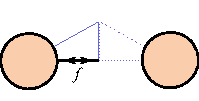
\includegraphics[width=0.43\textwidth]{diffuse7diskFundDflips2}
(b)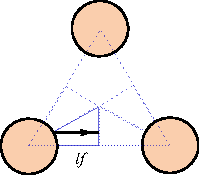
\includegraphics[width=0.43\textwidth]{diffuse7diskFundDflips3}
\\
(c)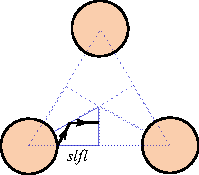
\includegraphics[width=0.43\textwidth]{diffuse7diskFundDflips6}
\end{center}
\caption{
(a) Elementary cell short 2-cycle , with multiplicity 3 corresponds to
the fixed pint $f$ in fundamental domain, $\cycle{02}=\cycle{f^2}$;
(b) Elementary cell short clockwise 3-cycle $\cycle{084}$, and
counterclockwise 3-cycle $\cycle{048}$, in
fundamental domain $\cycle{048}=\cycle{(\ell f)^3}$.
(c) Elementary cell short 6-cycle of multiplicity 2, in
fundamental domain $\cycle{0\underline{10}8642}=\cycle{(s\ell f\ell )^6}$.
    }
\label{7diskFundDflips2A}
\end{figure}
%%%%%%%%%%%%%%\item[Figure 4]%%%%%%%%%%%%%%%%%%%%%%%%%%%%%%%%%%%%%%%%%%

This is no new the 2-cycle:
$ \cycle{s \ell f \ell f \ell}
= \cycle{s f \ell f f \ell}
= \cycle{s f}
\neq \cycle{046\underline{10}}$,

There is also 2-cycle $\cycle{0369}$ (once we start including longs).

\begin{figure}
\includegraphics[width=\textwidth]{cycle026}
\caption{3-cycle \cycle{026} for $w=0.3$ (left) and $w=2$ (right). }
\label{fig:cycle026A}
\end{figure}

% \item[2014-07-11 Tingnan]
I have checked a few cycles and their new symbolic representations. For
example, $\cycle{026}$ and \cycle{0260628}. For cycle $\cycle{026}$ and
$w=0.3$, \reffig{fig:cycle026A}\,(left panel),
the symbolic sequence is $\cycle{f\ell sf\ell f fs}$.
% \item[2014-07-14 Predrag]
Using $f f = 1$
\[
\cycle{f\ell sf\ell f fs}
    = \cycle{f\ell sf\ell s}
    = \cycle{f\ell s}
\,.
\]
For $w=2.0$, \reffig{fig:cycle026A}\,(right panel), the
sequence is slightly different, $f\ell s\ell f \ell fs$, but with the
equivalence relations
% $f \ell f=\ell f \ell$
% \item[2014-07-14 Predrag]
% You are sure that $f\ell f$ equals $\ell f \ell$?
% The have different numbers of flips.
$f s = s f$ and $f \ell f = \ell f \ell$ the end sequence is the
same,
\[
\cycle{f\ell s\ell f \ell fs}
    = \cycle{\ell s\ell f \ell s}
    = \cycle{\ell s f \ell f s}
    = \cycle{\ell s f}
\,.
\]

% \item[2014-07-11 Tingnan]
Similar results can be obtained for $\cycle{0260628}$ in
\reffig{fig:cycle0260628A}.
\[
\cycle{f \ell f s f \ell ...}
\,.
\]
(2014-07-14 Predrag: I give up, let computer do this...)
I have also
checked a few cases when long flights are involved, and the same
conclusion holds: the symbolic sequence we proposed is invariant to
parameter changes.

\begin{figure}
\includegraphics[width=\textwidth]{cycle0260628}
\caption{\label{fig:cycle0260628A}
7-cycle \cycle{0260628} for $w=0.3$ (left) and $w=2$ (right).
}
\end{figure}

\begin{table}
\begin{center}
\begin{tabular}{r}
Symbols and itinerary \\\hline
$\ell$  \\
$s\ell$ \\
$\ell s \ell$ \\
$s \ell s \ell$ \\
$\ell s \ell s \ell$ \\
$s\ell s \ell s \ell$ \\
$s$  \\
$\ell s$ \\
$s \ell s $ \\
$\ell s \ell s$ \\
$s \ell s \ell s$ \\
- \\\hline
\end{tabular}
\end{center}
\caption{All 11 combinations without flip $f$. }
\label{tab:11slcombos}
\end{table}
(2014-07-17 Tingnan) Obervation: since the free flight cannot cross over a disk, the sequence $sl$ or $ls$ can at most appear 3 times, and the $C^6=e$ relation can be re-written as $(s\ell)^3=(\ell s)^3$ (i.e. rotating 180 degree either clockwise or counter clockwise would give the same tile). This also reduces the number of symbols in the state machine(Fig.~\ref{fig:statemachine}). Following the graph, We can generate at most 11 strings without flip $f$(Table ~\ref{tab:11slcombos}). For a single flip, $f$ can be sandwiched by
any two of the combinations (including the $-$ as a place holder). A valid (and longer) sequence can be generated according to the graph.
\begin{figure}
(a)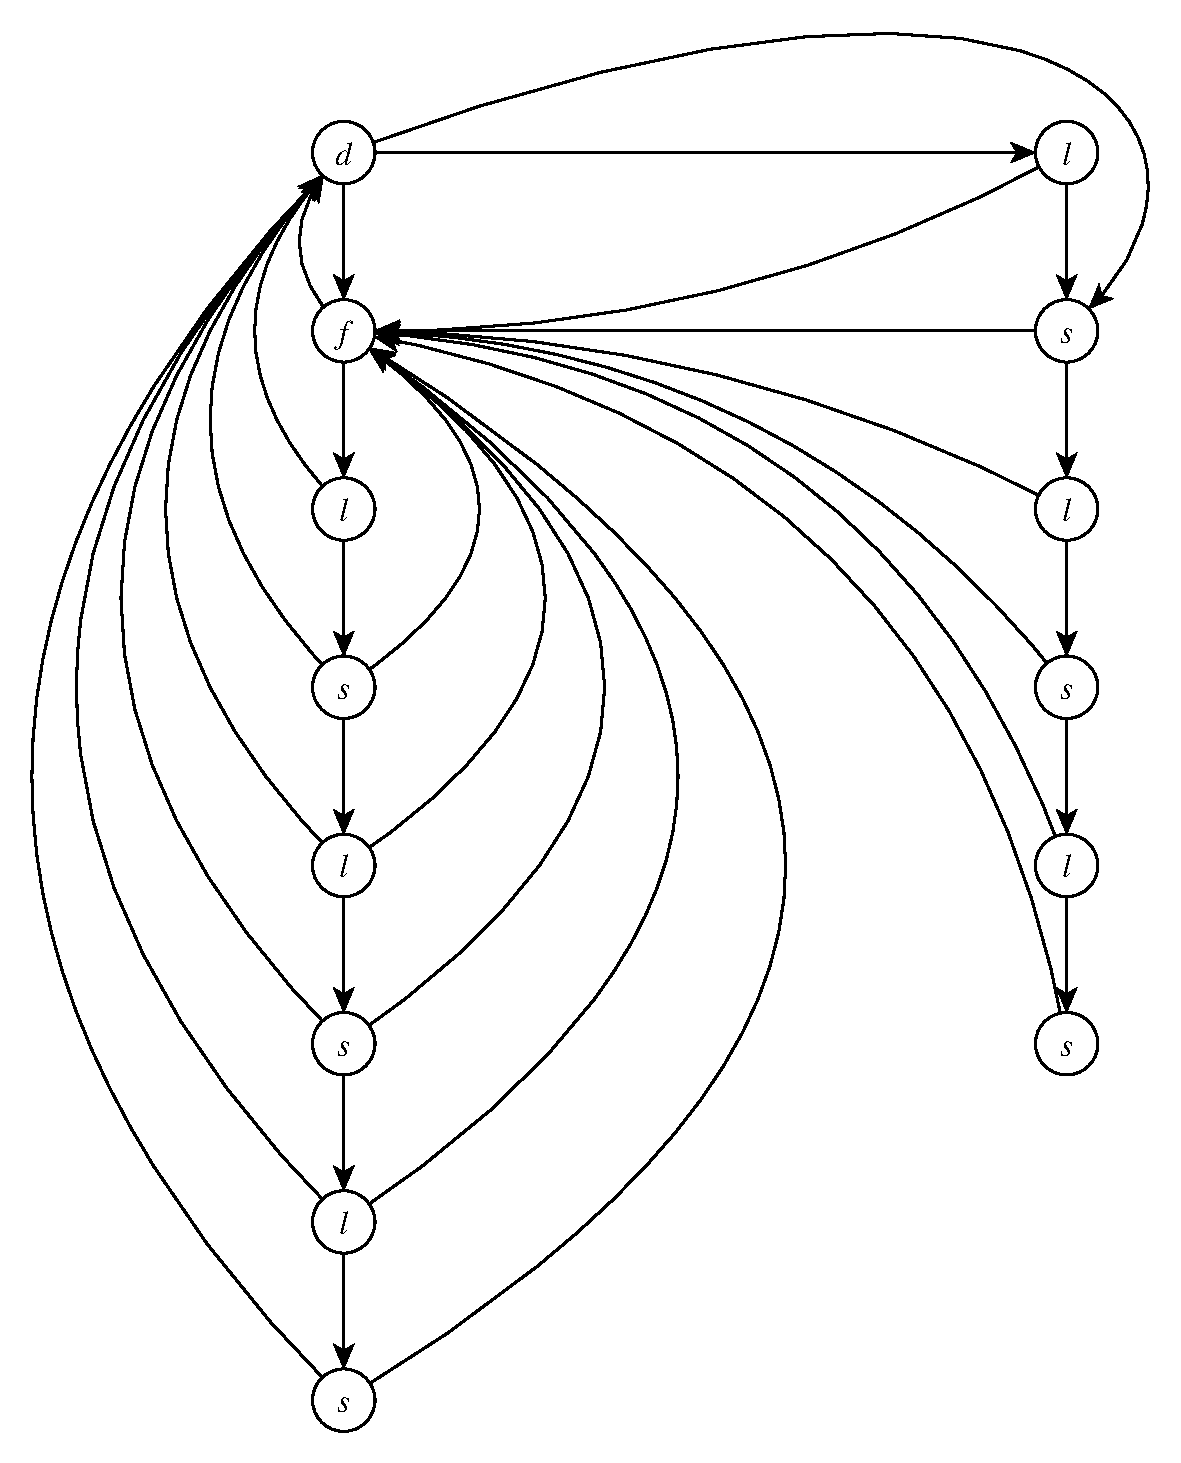
\includegraphics[width=0.5\textwidth]{diffuseStatemachine}
(b)\includegraphics[width=0.5\textwidth]{statemachine_finitehorizon}
\caption{\label{fig:statemachine} The Markov graph for the symbols.
}
\end{figure}

As soon as the horizon becomes finite the longest free flight without $f$
is $\ell s \ell$. $s \ell s$ is prohibited by the closed horizon. We also
have additional pruning rules for a flight between two nearest disks:
(A), only one $f$ could appear. (B), $ \ell s \ell $ is forbidden because
flight like this cannot hit nearest disk. With those rules we can
generate grammatically allowed symbol sequence:
\[
\overbrace{-,\ell,s\ell}\, f\,\overbrace{-,\ell,s,\ell s, s\ell}\, d
\]

There are 12 physically allowed combinations, see \reftab{tab:12symbols}.
They are labeled in \reffig{fig:12shortflight}.
\begin{table}
\begin{center}
\begin{tabular}{c|r|c}
\# & Itinerary & corresponding cycle\\\hline
0&$fd$ & \cycle{06} \\
1&$\ell fd$ & \cycle{048} \\
2&$s\ell fd$ & \cycle{24} \\
3&$f\ell d$  & time reversal of $\ell fd$\\
4&$\ell f\ell d$ & ? \\
5&$s\ell f\ell d$ & \cycle{0\underline{10}8642}\\
6&$fsd$  & ?  \\
7&$\ell fsd$ & \cycle{26} = \cycle{08} \\
8&$fs\ell d$ & time reversal of $\ell fsd$ (notice all $fs$ is replaced by $sf$)\\
9&$f\ell sd$  & time reversal of $s\ell fd$\\
10&$\ell f\ell sd$ & time reversal of $s\ell f\ell d$ \\
11&$s\ell f\ell sd$ & ? \\
\hline
\end{tabular}
\end{center}
\caption{All 12 combinations to visit nearest disk(s). }
\label{tab:12symbols}
\end{table}
\begin{figure}
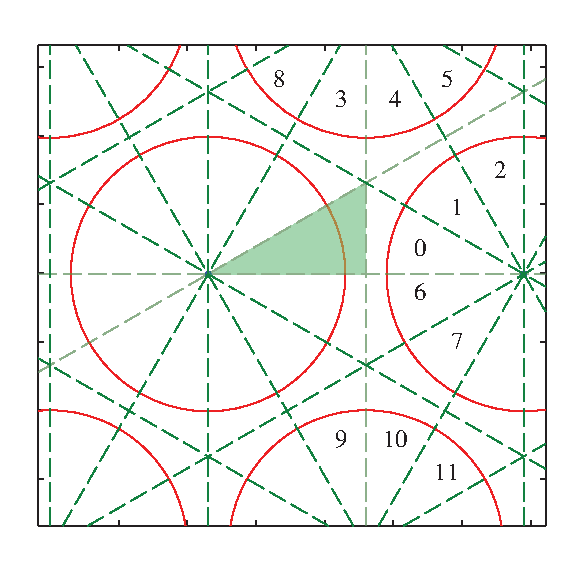
\includegraphics[width=0.5\textwidth]{diffuse12shortflight}
\caption{\label{fig:12shortflight} 12 possible short flights when horizon is finite.
}
\end{figure}

{\bf 2014-07-20 Predrag}:
I added $\cycle{fsd} =  \cycle{08}$ from a previous scribblings, please
recheck. Have not gone through your pruning rules yet.

{\bf 2014-07-21 Tingnan}:
You are right. I have corrected it in the table now. I am a bit confused because apparently I got more symbols than 6. If we shrink the size of the disk and impose finite horizon we have a total of 18 valid sequences to visit the 3 nearest disks (we have also to remove a marginal sequence that actually is a free parallel flight). However, the pruning here is also strong.

{\bf 2014-08-18 Tingnan}:

We started to notice that any string combination would map the current fundamental domain to a new one. With imposed finite horizon (suppose we can only hit at most 12 disks starting from any disk), and there are a limited number of new fundamental domains that can be mapped from current one before collision. Because disks cannot be penetrated, there are a total of 36 fundamental domains available starting from the current one, see Figure~\ref{fig:36symbols} and Table~\ref{tab:36symbols}. It looks like we have more than 12 symbols, but the pruning here is severe, see Fig.~\ref{fig:fdSymbolPruning}.
\begin{figure}
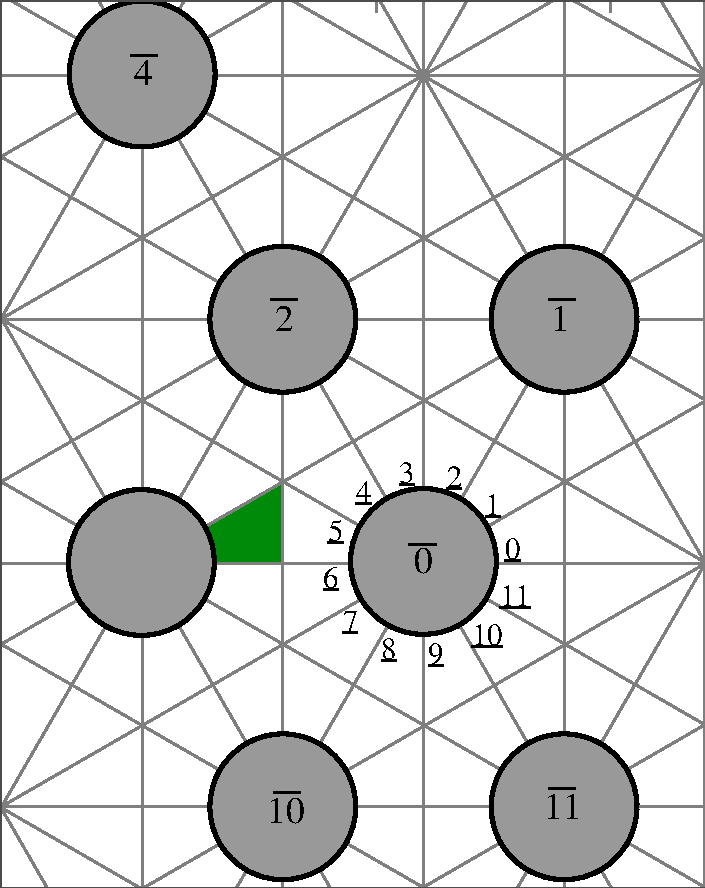
\includegraphics{diffuseFDSymbolIllustration}
\caption{Accessible triangular domains from the current one (marked in green). The underscored numbers represent the disk label with respect to the elementary cell. For each disk, the fundamental domains are labeled counter clockwise from 0 to 11. So each triangular region (fundamental domain) can be uniquely identified by the combination of a disk label and a partition label.}
\label{fig:36symbols}
\end{figure}
\begin{table}
\begin{center}
\begin{tabular}{c|r}
disk label & partition label \\\hline
$\underline{0}$& 3,4,5,6,7,8\\
$\underline{2}$& 5,6,7,8,9,10\\
$\underline{10}$& 1,2,3,4,5,6\\
$\underline{1}$& 4,5,6,7,8,9\\
$\underline{3}$& 6,7,8,9,10,11\\
$\underline{11}$& 2,3,4,5,6,7\\
\hline
\end{tabular}
\end{center}
\caption{All 12 combinations to visit nearest disk(s). }
\label{tab:36symbols}
\end{table}
\begin{figure}
\includegraphics[width=\textwidth]{pruningRuleIllustration}
\caption{Pruning rule for the fundamental domain. After flight $\underline{0}-5$, there are only 9 (including the edges) domains accessible on the nearest disks (plus 6 partitions on disk $\underline{1}$, which is not shown here). On average there are around 12 symbols that are not pruned.}
\label{fig:fdSymbolPruning}
\end{figure}

{\bf 2014-09-08 Tingnan}:
I have successfully computed all cycles in the fundamental domain upto length 5; Here are the results (Table.~\ref{tab:fddomaincycleaverage}). Notice in Schreiber paper $\zeta(0, 0)$ for $n_p = 1$ differs from my result by $1$ (he might forgot add the constant 1 for the calculation). My calculation matches the previous result up to cycle length 2. From cycle length 3 I begin to include more cycles and the results are slightly different.

\begin{table}[htbp]
  \centering
  \caption{\Dzeta\ cycle expansion estimates of
  the mean flight time
  $\spaceAver{\period{}}_\zeta
  =\sum^{\prime}(-1)^{k}(\tau_{p_1}+\cdots+\tau_{p_k})/\vert\ExpaEig_{p_1}\cdots\ExpaEig_{p_k}\vert$,
  mean log of the expanding Floquet multiplier
  $\spaceAver{\ln\ExpaEig}_\zeta
  =\sum^{\prime}(-1)^{k}(\mu_{p_1}+\cdots+\mu_{p_k})/\vert\ExpaEig_{p_1}\cdots\ExpaEig_{p_k}\vert$,
  the Lyapunov exponent $\lambda = \spaceAver{\ln\ExpaEig}_\zeta / \spaceAver{\period{}}_\zeta$ and the dynamical zeta function $\zeta(0,0)$.}
    \begin{tabular}{c|r|r|r|r|r}
    $n_p$ & \# cycles & $\spaceAver{\period{}}_\zeta$
               & $\spaceAver{\ln\ExpaEig}_\zeta$
                        & $\lambda$
                                 & $\zeta(0,0)$ \\
    \hline
    1 & 5 & 1.097954 & 1.528281 & 1.391935 & -0.216976 \\
    2 & 10 & 0.627470 & 1.095191 & 1.745407 & -0.024823 \\
    3 & 33  & 0.614226 & 1.057914 & 1.722350 & -0.022196 \\
    4 & 108 & 0.540654 & 0.943171 & 1.744502 &  0.000219 \\
    5 & 373 & 0.521036 & 0.917438 & 1.760797 &  0.002346 \\
    \end{tabular}%
  \label{tab:fddomaincycleaverage}%
\end{table}

% compile by  pdflatex blog; biber blog
% GitHub cvitanov/reducesymm/dasgroup/dailyBlog.tex


\chapter{Daily group theory blog}
\label{s-groupTheBlog}



\begin{description}

\item[2003-02-05  Bhama Srinivasan] <srinivas@uic.edu>
The reference to an early use of diagrammatic notation is R.
Brauer\rf{Brauer1937} {\em On algebras which are connected with the
semisimple continuous groups} in 1937. The algebra he constructs is now
called the Brauer algebra (essentially birdtracks for SO/Sp:1), but people
now study it algebraically. I had a student who worked on it and found a nice
basis for it in his Ph.D thesis.

\item[2003-03-19  Dirk Kreimer] told me to
read these (perhaps they belong to the QFT blog):

Lavelle and D. McMullan\rf{LavMcM97}
(Predrag not sure if this is the right one, they have many articles together.
Could also be \refrefs{BaLaMcM97,BaLaMcM98})

Suslov\rf{Suslov99}

Rota: On combinatoric (book)
	article on Moebius Function

%\HREF{http://www.yahoo.groups.com}{www.yahoo.groups.com}

\item[2015-12-02  Predrag]
Should one study
Klink and Wickramasekara\rf{KliWic15},
{\em Relativity, Symmetry and the Structure of Quantum Theory I} ?
They say: ``The history of how quantum mechanics was developed is a
fascinating one and underlies the focus of this book; namely, given the
rules that the founders of quantum mechanics developed, is it possible to
find principles that lead to the structure of quantum mechanics as it was
historically formulated? This is the first book in a series of works
considering what particular relativity is applicable to a given dynamical
theory. The series considers Newton, Einstein, and de Sitter
relativities, while this book examines the unitary irreducible
representations of the Galilei group and see how they provide the
framework for Galilean quantum theory.
''

\item[2015-12-02  Predrag] Abbas\rf{Abbas16} {\em Group Theory
in Particle, Nuclear, and Hadron Physics} will be available in July 2016.

\item[2016-04-03 Predrag] I've collected a bunch of group theory e-books,
saved them in \wwwcb{/library}:

Bincer12.pdf\rf{Bincer12}

Ramond10.pdf\rf{Ramond10}

isham99.pdf\rf{isham99}

MaGu04.pdf\rf{MaGu04}

Dresner98.pdf\rf{Dresner98}

Yaglom88.pdf\rf{Yaglom88}

DasOkubo14.pdf\rf{DasOkubo14}

Fecko06.pdf\rf{Fecko06}
{\em Differential Geometry and Lie Groups for Physicists},

Bergman98.pdf

\HREF{https://www.scribd.com/doc/207786199/Q-HO-KIM-Group-Theory-A-Physicist-s-Primer}
{Ho-Kim14.pdf} {\em  Group Theory - A Physicist's Primer}, just lecture
notes.

From Shlomo Sternberg
\HREF{http://www.math.harvard.edu/~shlomo/}{online books}:
Sternberg04.pdf {\em Lie algebras}


\end{description}


%\newpage %%%%%%%%%%%%%%%%%%%%%%%%%%%%%%%%%%%%%%%%%%%%%%%%
\printbibliography[heading=subbibintoc,title={References}]



\end{document}
